\documentclass[a4paper,12pt]{report}
\usepackage[francais]{minitoc}
\usepackage{ucs}
\usepackage[utf8x]{inputenc}
\setcounter{minitocdepth}{1}
\setcounter{parttocdepth}{2}
\setlength{\ptcindent}{0pt}
\renewcommand{\ptcfont}{\normalsize\rmfamily\upshape\mdseries}
\renewcommand{\ptcCfont}{\normalsize\rmfamily\upshape\bfseries}
\setcounter{minitocdepth}{2} 
\setlength{\mtcindent}{24pt}
\newcommand{\mtcskipamount}{\bigskipamount}
\usepackage[french]{babel}
\usepackage{tikz}
\small
%\usepackage[latin1]{inputenc} 
%\usepackage[T1]{fontenc}

%\renewcommand{\ptcSfont}{\normalsize\rmfamily\upshape\mdseries}
 
%\setlength{\mtcskipamount}{\bigskipamount}
%\renewcommand{\mtcfont}{\small\rmfamily\upshape\mdseries}
%\renewcommand{\mtcSfont}{\small\rmfamily\upshape\bfseries}

%\newcommand{\textlbrackdbl}[]
%\setcounter{minitocdepth}{2} 
%\setlength{\mtcindent}{24pt} 
%\setlength{\mtcskipamount}{\bigskipamount}
%\renewcommand{\mtcfont}{\small\rmfamily\upshape\mdseries}
%\renewcommand{\mtcSfont}{\small\rmfamily\upshape\bfseries}
%\usepackage{french}
%\setcounter{parttocdepth}{2}
%\setlength{\ptcindent}{0pt}
%\renewcommand{\ptcfont}{\normalsize\rm}
%\renewcommand{\ptcCfont}{\normalsize\bf}
%\renewcommand{\ptcSfont}{\normalsize\rm}

%%%%%%%%%%%%%% Definitions %%%%%%%%%%%%%%
\def\onehalf{\textstyle{\frac{1}{2}}}
 \def\D{{\mathcal D}{}}
 \def\Gammabol{{\stackrel{\circ}{\Gamma}}{}} 
 \def\gammabol{{\stackrel{\circ}{\Gamma}}{}}
 \def\Abol{{\stackrel{~\circ}{A}}{}}
 \def\Rbol{{\stackrel{\circ}{R}}{}}
 \def\Lbol{{\stackrel{\circ}{\mathcal L}}{}}
 \def\Tbol{{\stackrel{\circ}{T}}{}}
 \def\Dbol{{\stackrel{\circ}{\mathcal D}}{}}
 \def\nabol{{\stackrel{\circ}{\nabla}}{}}
 \def\jbol{{\stackrel{\circ}{\jmath}}{}}
 \def\Gammaw{{\stackrel{\bullet}{\Gamma}}{}}
 \def\Omegaw{{\stackrel{\bullet}{\Omega}}{}}
 \def\Aw{{\stackrel{~\bullet}{A}}{}}
 \def\Vw{{\stackrel{\bullet}{V}}{}}
 \def\Rw{{\stackrel{\bullet}{R}}{}}
 \def\Qw{{\stackrel{\bullet}{Q}}{}}
 \def\jw{{\stackrel{\bullet}{\jmath}}{}}
 \def\tw{{\stackrel{\bullet}{t}}{}}
 \def\L{{\mathcal L}{}}
 \def\Lw{{\stackrel{\bullet}{\mathcal L}}{}}
 \def\Tw{{\stackrel{\bullet}{T}}{}}
 \def\Kw{{\stackrel{\bullet}{K}}{}}
 \def\nablaw{{\stackrel{\bullet}{\nabla}}{}}
 \def\Dw{{\stackrel{\bullet}{\mathcal D}}{}}
 \def\dw{{\stackrel{\bullet}{D}}{}}
 \def\Sw{{\stackrel{\bullet}{S}}{}}
 \def\be{\begin{equation}}
 \def\ee{\end{equation}}
 \def\ba{\begin{eqnarray}}
 \def\ea{\end{eqnarray}}
 \def\nn{\nonumber}
 % d'Alembertian definition
 \def\qed{\hbox{${\vcenter{\vbox{%HOLLOW SQUARE
    \hrule height 0.4pt\hbox{\vrule width 0.4pt height 6pt
    \kern5pt\vrule width 0.4pt}\hrule height 0.4pt}}}$}}
 \def\qedw{{\stackrel{\bullet}{\qed}}{}}
%\usepackage[T1]{fontenc}
%\usepackage[pctex32]{graphics}
%%%%%%%%%%%%%%%%%fin d\'efinition%%%%%%%%%%%%%%%%%%%%%%%%%%%%%%%%%%%%%
%%%%%%%%%%%%%%%%%%%%%%%%%%%%%%%%%%%%%%%%%%%%%%%%%%%%%%%%%%%%%%%
%\usepackage[lmargin=4cm,rmargin=2.5cm]{geometry}
\def\eps{\epsilon}
\def\f{\frac}
\def\cN{{\mathcal N}}
\def\cC{{\mathcal C}}
\def\nn{\nonumber}
\newcommand{\rot}{\mathop{\rm rot}\nolimits}
\newcommand{\dive}{\mathop{\rm div}\nolimits}
%\newcommand{\\mbox{diam}}{\mathop{\rm \mbox{diam}}\nolimits}
\def\bv{\textbf{v}}
\def\bw{\textbf{w}}
\def\bu{\textbf{u}}
\def\bH{\textbf{H}}
\def\bn{\textbf{n}}
\def\bt{\textbf{t}}
\def\Om{\Omega}
\def\bff{\textbf{f}}
\def\cT{{\mathcal T}}
%\newcommand{\cT}{\mathcal{T}}
%-------------------------------------------------

%-------------------------------------------------


\usepackage{amstext,amsmath,amssymb,amsfonts}

\usepackage{eucal,rotating}
\usepackage{float}


\usepackage{setspace}
%------------------------------interligne verticale---------------------------
\onehalfspacing 
\makeatletter 
\newcommand{\LyX}{L\kern-.1667em\lower.25em\hbox{Y}\kern-.125emX\spacefactor1000} 
\makeatother
% \usepackage{hyperref}
% \usepackage{hyperref}
%\usepackage[top=2cm, bottom=2cm, left=2cm, right=2cm]{geometry}
%\usepackage[table]{xcolor}
%\usepackage{color}
\usepackage{multirow}
\usepackage{ctable}

% \usepackage[pdftex=true,
%   hyperindex=true,
%   colorlinks=true]{hyperref} 
% Couleurs des liens plus propre et plus joli!!!
% \hypersetup{
% 	colorlinks,%
% 	citecolor=blue,%
% 	filecolor=black,%
% 	linkcolor=black,%
% 	urlcolor=blue}

\addtolength{\hoffset}{-0.7cm}

\addtolength{\textwidth}{1.7cm}%1.6avant
\addtolength{\voffset}{-2.cm}
\addtolength{\textheight}{2cm}

%\addtolength{\textwidth}{1.7cm}%1.6avant
%\addtolength{\voffset}{-3.2cm}
%\addtolength{\textheight}{2cm}

%jusqu'ici
%avant il y avait ca
\usepackage{color}
%%\usepackage[all]{xy}
%\usepackage[centertags]{amsmath}
%\usepackage{latexsym}
% \usepackage{stmaryrd}
%jusqu icib

\usepackage{amsfonts}
\usepackage{amsmath}
\usepackage{amscd}
\usepackage{array}
\usepackage{multirow}
\usepackage{mathrsfs}
%\usepackage{multicolumn}
%avant il y avait ca

\usepackage{amssymb}
\usepackage{amsthm}

\frenchspacing  \linespread{1.5}%1.5avant
\usepackage{fancyhdr}
\pagestyle{fancy}
\usepackage[dvips]{epsfig}

%jusqu ici

\usepackage{graphicx}
\usepackage{t1enc}
%\usepackage[latin1]{inputenc}
\usepackage[french]{babel}

\usepackage{amscd}
\usepackage{graphics}
\setlength{\unitlength}{1mm}

%%%%%%%%%%%%%%%%%%%%%%%%%%%%%%%%%%%%%%%%%%%%%%%%%%%%%%%%%%%%%%%%%%%%%%%%%%%%%%%%%%%%%%%%%%%%%%%%%%%%%%%%%%%%%%%%%%%%%%%%%%
%%%%%%%%%%%%%%%%%%%%%%%%%%%%%%%%%%%%%%%%%%%%%%%%%%%%%%%%%%%%%%%%%%%%%%%%%%%%%%%%%%%%%%%%%%%%%%%%%%%%%%%%%%%%%%%%%%%%%%%%%%%%?
%%%%%%%%%%%%%%%%%%%%%%%%%%%%%%%%%%%%%%%%%%%%%%%%%%%%%%%%%%%%%%%%%%%%%%%%%%%%%%%%%%%%%%%%%%%%%%%%%%%%%%%%%%%%%%%%%%%%%%%%%%%



%
% \setlength{\headheight}{14pt}  %%
% \setlength{\oddsidemargin}{0pt} %%{52pt} %%
% \setlength{\evensidemargin}{0pt}       %%{10pt} %%
% \setlength{\marginparwidth}     {72pt}%%{72pt}
% \pagestyle{headings}
% \linespread{1.13}
% \textheight 22cm
% \textwidth 18cm
% \hoffset -.9 cm
%  \voffset -0.9 cm
%  \def\dessous#1\sous#2{\mathrel{\mathop{\kern0pt#2}\limits_{#1}}}
% \normalbaselineskip=18pt
% \normalbaselines
%
% \parindent.5cm
% \parskip=5pt
%%%%%%%%%%%%%%%%%%%%%%%%%%%%%%%%%%%%%%%%%%%%%%%%%%%%%%%%%%%%%%%%%%%%%%%%%%%%%%%%%%%%%%%%%%%%%%%%%%%%%%%%%%%
%%%%%%%%%%%%%%%%%%%%%%%%%%%%%%%%%%%%%%%%%%%%%%%%%%%%%%%%%%%%%%%%%%%%%%%%%%%%%%%%%%%%%%%%%%%%%%%%%%%%%%%%%%%?
%%%%%%%%%%%%%%%%%%%%%%%%%%%%%%%%%%%%%%%%%%%%%%%%%%%%%%%%%%%%%%%%%%%%%%%%%%%%%%%%%%%%%%%%%%%%%%%%%%%%%%%%%%%%


%%%%%%%%%%%%%%%%%%  Sommaire   %%%%%%%%%%%%%%%%%%
%\usepackage[french]{minitoc}

%\dominitoc
%\dominilof
%\dominilot
%\usepackage[english]{minitoc}
%\setcounter{minitocdepth}{1}
\setcounter{tocdepth}{3}


    %\usepackage[francais]{minitoc}
%    \setcounter{minitocdepth}{4}
    \usepackage{setspace}
    \usepackage{float}


%%%%%%%%%%%%%%%%%%%%%%%%%%%%%%%%%%%%%%%%%%%%%%%%%%%%%%%%%


%\usepackage[english]{babel}
%\usepackage[english,french]{babel}
%\usepackage[french]{babel}

\makeatletter
\newcommand{\thechapterwords}
{ \ifcase \thechapter\or Un\or Deux\or Trois\or Quatre\or
Cinq\or Six\or Sept \or Huit\or Neuf\or Dix\or Onze\fi}
\def\thickhrulefill{\leavevmode \leaders \hrule height 1ex \hfill \kern \z@}
\def\@makechapterhead#1{%
  %\vspace*{50\p@}%
  \vspace*{15\p@}%
  {\parindent \z@ \centering \reset@font
        \thickhrulefill\quad
        \scshape \@chapapp{} \thechapterwords
        \quad \thickhrulefill
        \par\nobreak
        \vspace*{15\p@}%
        \interlinepenalty\@M
        \hrule
        \vspace*{15\p@}%
        \Huge \bfseries #1\par\nobreak
        \par
        \vspace*{15\p@}%
        \hrule
    \vskip 60\p@
    %\vskip 100\p@
  }}
\def\@makeschapterhead#1{%
  %\vspace*{50\p@}%
  \vspace*{15\p@}%
  {\parindent \z@ \centering \reset@font
        \thickhrulefill
        \par\nobreak
        \vspace*{15\p@}%
        \interlinepenalty\@M
        \hrule
        \vspace*{15\p@}%
        \Huge \bfseries #1\par\nobreak
        \par
        \vspace*{15\p@}%
        \hrule
    \vskip 60\p@
    %\vskip 100\p@
  }}
  \def\@makechapterhead#1{%
  %\vspace*{50\p@}%
  \vspace*{15\p@}%
  {\parindent \z@ \centering \reset@font
        \thickhrulefill\quad
        \scshape \@chapapp{} \thechapterwords
        \quad \thickhrulefill
        \par\nobreak
        \vspace*{15\p@}%
        \interlinepenalty\@M
        \hrule
        \vspace*{15\p@}%
        \Huge \bfseries #1\par\nobreak
        \par
        \vspace*{15\p@}%
        \hrule
    \vskip 60\p@
    %\vskip 100\p@
    }}
  \frenchspacing \pagestyle{headings}
%%avant c etait \frenchspacing  \linespread{1.1}%1.5avant
%%d?finition des ent?tes
\usepackage{fancyhdr}
\pagestyle{fancy}

%avant il y avait ca
 %\usepackage[dvips]{epsfig}
%jusqu ici

% Ceci permet d?avoir les noms de chapitre et de section
% en minuscules
%avant il y avait ca
\renewcommand{\sectionmark}[1]{\markboth{#1}{}}
\renewcommand{\sectionmark}[1]{\markright{\thechapter\ #1}}


\renewcommand{\sectionmark}[1]{\markboth{#1}{}}
%\renewcommand{\chaptermark}[1]{\markboth{#1}{}}
%\renewcommand{\sectionmark}[1]{\markright{\thesection\ #1}}
\fancyhf{} % supprime les en-t?tes et pieds pr?d?finis
\fancyhead[L,R]{\bfseries\thepage}% Left Even, Right Odd
\fancyhead[L]{\bfseries\rightmark} % Left Odd
\fancyhead[R]{\bfseries\leftmark} % Right Even
\renewcommand{\headrulewidth}{1pt}% filet en haut de page
\addtolength{\headheight}{14pt} % espace pour le filet (avant on avait 1pt
\renewcommand{\footrulewidth}{1.5pt}% filet en bas de page
%\addtolength{\footheight}{0.5pt} % espace pour le filet en bas
\fancypagestyle{plain}{ % pages de tetes de chapitre
\fancyhead{} % supprime l'entete
%\fancyfoot{} %supprime le pied de page
\renewcommand{\headrulewidth}{0pt}
}
\newcommand{\clearemptydoublepage}{%
\newpage{\pagestyle{plain}\cleardoublepage}}

\rhead{\textbf{\thepage}}
\lhead{\textsl{\leftmark}}

%\fancyfoot[LE, RO]{\tiny \textbf{Bakary MANGA \copyright URMPM/IMSP 2008}}
\fancyfoot[L, RO]{\tiny \textbf{ Anselme HADO    2021
                                 \\ anselmehado85@yahoo.com}}
% % \fancyfoot[L, RO]{\tiny \textbf{Andr\'e DEMBELE \copyright URMPM/IMSP 2010}}
\fancyfoot[LO]{\tiny \emph{  \textbf{
L'acc\'el\'eration de l'Univers et mod\`eles de gravit\'e
}   }}
\fancyfoot[RE]{\tiny \textsl{Math\'ematique}}

 \rhead{\textbf{\thepage}}
\lhead{\textsl{\leftmark}}
\usepackage{newlfont}

%\usepackage[active]{srcltx}
\hfuzz2pt
\newlength{\defbaselineskip}
\setlength{\defbaselineskip}{\baselineskip}
\newcommand{\setlinespacing}[1]%
           {\setlength{\baselineskip}{#1 \defbaselineskip}}
%\newcommand{\doublespacing}{\setlength{\baselineskip}%
                     %      {1.5 \defbaselineskip}}
%\newcommand{\singlespacing}{\setlength{\baselineskip}{\defbaselineskip}}
\newtheorem{remark}{Remark}[section]
\newenvironment{prof}[1][Preuve]{\textbf{#1.} }{\ \rule{0.5em}{0.5em}}
\theoremstyle{plain}
%serge
\newtheorem{thm}{Th\'eor\`eme}[chapter]
\newtheorem{cor}[thm]{Corollaire}
\newtheorem{lem}[thm]{Lemme}
\newtheorem{pro}[thm]{Proposition}
\newtheorem{hypo}[thm]{Hypoth\`ese}
\newtheorem{nota}[thm]{Notation}
%\theoremstyle{definition}
\newtheorem{dfn}[thm]{D\'efinition}
\newtheorem{rap}{Rappel}[chapter]
%\theoremstyle{remark}
\newtheorem{rmq}[thm]{Remarque}
%\newtheorem{nota}[thm]{Notations}
%\numberwithin{equation}{section}
%\theoremstyle{definition}
\newtheorem{expl}[thm]{Exemple}

%bakary
%\newtheorem{lemma}{Lemma}[section]
%\newtheorem{exercise}{Exercice}[section]
%\newtheorem{proposition}{Proposition}[section]
%\newtheorem{theorem}{Theorem}[section]
%\newtheorem{definition}{Definition}[section]
%\newtheorem{corollary}{Corollary}[section]
%\newtheorem{notation}{Notation}[section]
%\newtheorem{example}{Example}[section]
%\newtheorem{property}{Propri?©t?©}[section]
%\newtheorem{theodef}{Theorem and Definition}[section]
%\newtheorem{rap}{Rappel}[section]





%%%%%%%%%%%%%%%%%%%%%%%%%%%%%%%%%%%%%%%%%%%%%%%%%%%%%%%%%%%%%%%%%%%
\newcommand{\al}{\alpha}
%\newcommand{\be}{\beta}
\newcommand{\p}{\partial}
\newcommand{\pr}{\prime}
\newcommand{\mbb}{\mathbb}
\newcommand{\mbf}{\mathbf}
\newcommand{\mc}{\mathcal}
\newcommand{\mf}{\mathfrak}
\newcommand{\mi}{\mathit}
\newcommand{\nb}{\nonumber}
\newcommand{\ti}{\textit}
\newcommand{\T}{\mathcal{T}}
\newcommand{\ben}{\begin{enumerate}}
\newcommand{\een}{\end{enumerate}}
\newcommand{\brap}{\begin{rap}}
\newcommand{\erap}{\end{rap}}
\newcommand{\bnota}{\begin{nota}}
\newcommand{\enota}{\end{nota}}
%%%%%%%%%%%%%%%%%%%%%%%%%%%%%%%%%%%
\newcommand{\beqs}{\begin{eqnarray}}
\newcommand{\eeqs}{\end{eqnarray}}
\newcommand{\ms}[1]{\mathsf{#1}}
\newcommand{\bs}{\symbol{92}}
%%%%%%%%%%%%%%%%%%%%%%%%%%%%%%%%%%%%%%%%%%%%%%%%%%%%%%%%%%%%%%%%
\newcommand{\n}{\nabla}
\newcommand{\noi}{\noindent}
\newcommand{\beq}{\begin{eqnarray}}
\newcommand{\eeq}{\end{eqnarray}}
\newcommand{\bpro}{\begin{pro}}
\newcommand{\epro}{\end{pro}}
\newcommand{\blem}{\begin{lem}}
\newcommand{\elem}{\end{lem}}
\newcommand{\bdfn}{\begin{dfn}}
\newcommand{\edfn}{\end{dfn}}
\newcommand{\bcor}{\begin{cor}}
\newcommand{\ecor}{\end{cor}}
\newcommand{\bthm}{\begin{thm}}
\newcommand{\ethm}{\end{thm}}
\newcommand{\bex}{\begin{expl}}
\newcommand{\eex}{\end{expl}}
\newcommand{\brmq}{\begin{rmq}}
\newcommand{\ermq}{\end{rmq}}
\newcommand{\bhypo}{\begin{hypo}}
\newcommand{\ehypo}{\end{hypo}}
%\newcommand{\benum}{\begin{enumerate}}
%\newcommand{\eenum}{\end{enumerate}}
\newcommand{\bitem}{\begin{itemize}}
\newcommand{\eitem}{\end{itemize}}
\newcommand{\cE}{\mathcal{E}}
%\newcommand{\curl}{\mathop{ curl}\nolimits}
%\newcommand{\dive}{\mathop{ div}\nolimits}
\theoremstyle{plain}
%\frenchspacing
\linespread{1}

%\usepackage[latin1]{inputenc}



\usepackage{graphicx}
\usepackage{t1enc}
% \hypersetup{
%        backref=true,                           % Permet d'ajouter des liens dans
%        pagebackref=true,                       % les bibliographies
%        hyperindex=true,                        % Ajoute des liens dans les index.
%        colorlinks=true,                        % Colorise les liens.
%        breaklinks=true,                        % Permet le retour ?  la ligne dans les liens trop longs.
%        urlcolor= blue,                         % Couleur des hyperliens.
%        linkcolor= blue,                        % Couleur des liens internes.
%        citecolor=blue,
%        bookmarks=true,                         % Cr\'e\'e des signets pour Acrobat.
%        bookmarksopen=true,                     % Si les signets Acrobat sont cr\'e\'es,
%                                                % les afficher compl\`etement.
%        pdftitle={Syst\`eme de facilitation des transactions portuaires},  % Titre du document.
%      % Informations apparaissant dans
%        pdfauthor={Andre},                      % dans les informations du document
%        pdfsubject={M\'emoire de fin de formation}           % sous Acrobat.
%     }

%%%%%%%%%%%%%%%%%%%%%%%%%%%%%%%%%%%%%  pdf interactive links %%%%%%%%%%%%%%%%%%%%%%%%%%%%%%%%%%%%%%%%%%%%
%  \definecolor{couleurliens}{rgb}{0.,0.,0.}% % "couleurliens" will contain black color
% \definecolor{couleurliens}{cmyk}{0.,0.,0.,0.} %other color see colorfile
% % % activation for links colors  in the pdf
\definecolor{couleurliens}{rgb}{0.,0.,1} % for sections, subsections and equations
 \definecolor{couleurliensref}{rgb}{0.1,0.,0.9} % for book and paper
\definecolor{couleurliensurl}{rgb}{.3,.4,.3} % for internet references
% \usepackage[pdftex,colorlinks=true,urlcolor=couleurliensurl,linkcolor=coul
% eurliens,
% citecolor=couleurliensref]{hyperref}



 \usepackage[pdftex,pdfmenubar=true,bookmarks=true,pdftoolbar=true]{hyperref}
\hypersetup{colorlinks,citecolor=red,filecolor=red,linkcolor=blue,urlcolor=cyan,pdftex}%permet de choisir la couleur des equation, refrence ...


%\setcounter{tocdepth}{0} % pour indiquer la profondeur de la table des mati\`eres
%%%%%%%%%%%%%%%%%%%%%%%%%%%%%%%%%%%%%%%%%%%%%%%%% end preamble %%%%%%%%%%%%%%%%%%%%%%%%%%%%%%%%%%55%%%%%
\linespread{1.1}
%%%%%%%%%%%%%%%%%%%%%%%%%%%%%%%%%%%%%%%%%%%%%%%%%%%%%%%%%%%%%%%%%%%%%%%%%%%%%%%%%%%%%%%%

\title{
%{\textbf{THEORIES ALTERNATIVES:\\ Th\'eorie N\'eo-Newtonienne,  
 %Th\'{e}orie T\'{e}l\'{e}parall\`{e}le G\'{e}n\'{e}ralis\'{e}e}} 
 }
\author{ 
%In\`es Godonou SALAKO
}
\date{ 
%Novembre 2013
}

%%%%%%%%%%%%%%%%%%%%%%%%%%%%%%%%%%%%%%%%%%%%%%%%%%%%%%%%%%%%%%%%%%%%%%%%%%%%%%%%%%%%%%%%
\begin{document}
%\begin{normalsize}
\begin{titlepage} 
%	\begin{flushleft}
%		
\includegraphics[scale=0.2]{logosm.png}
%	\end{flushleft} 
%	\begin{flushright}
%		
\includegraphics[scale=0.5]{logoUAC1.png}
%	\end{flushright}
	
	
		
	
% height= 2 cm, width=2.1cm
% height= 1.5 cm, width=2.1cm

 \begin{figure}
\includegraphics[scale=0.5]
 {logoUAC1.png}
 \hspace*{10cm}
 \ 
\includegraphics[scale=0.2]{logosm.png}
% \includegraphics[height= 2 cm, width=2cm]{ICTP.pdf}
 \end{figure}
\begin{center}
  Universit\'e d'Abomey-Calavi\\
{\bf Ecole Doctorale des Sciences Exactes et Appliqu\'ees }\\
Formation Doctorale Sciences des Mat\'eriaux\\[1cm]
\textbf{Memoire de Master}\\
\underline{{\bf Option}}: Physique Th\'eorique et Math\'ematique\\
\underline{{\bf Sp\'ecialit\'e}}: Cosmologie et gravitation
\end{center}
%\begin{center}
 %\textbf{TH\`ESE}
%\end{center}

\begin{center}
 %\rule{.8\textwidth}{.01pt}\\[0.3pt]
 \vspace{0.50cm}
  Réalisé  par:\\
 \vspace{0.5cm}
 \textbf{Anselme HADO }\\
 \begin{tabular}{|l|c|r|}
 \hline
 {\color{red}{\textbf{Titre}}}\\
 \hline
 \end{tabular}
\hrulefill
\begin{flushleft} 
\begin{center}
 \emph{{\color{black}\textbf{\small {L'acc\'el\'eration de l'Univers et mod\`eles de gravit\'e}}}}
 \end{center}
\end{flushleft} 
\hrulefill
 \vspace{0.20cm}
%\footnote{Support\'ee par le Centre International de la Physique Th\'eorique (Abdus Salam), Italie.
%by the Abdus Salam International Centre for Theoretical
%Physics (ICTP), Italy. %; %the 
%Japanese Government through the UNESCO-ICTP/IAEA/MORI and The Academy of Sciences for Developing World
%(TWAS)}
%\rule{.8\textwidth}{.01pt}\\[0.3pt]
\end{center}
%\vspace*{0.20cm}
%%%%%%%%%%%%%%%%%%%%%%%%%%%%%%%%%%%%%%%%%%%%%%%%%%%%%%%%%%%%%%%%%%%%%%%%%%%%%%%%%%%%%%%%%%%%%%%%%%%%%%%%%%%
\begin{center}
 \begin{tabular}{|l|c|r|}
 \hline
  {\color{red}{\textbf{Pr\'esident de jury}}} \\
 \hline
 \end{tabular}
\end{center}
\begin{center}
\small {\textbf{ Prof. },   \emph{ }}\\
\end{center}
%%%%%%%%%%%%%%%%%%%%%%%%%%%%%%%%%%%%%%%%%%%%%%%%%%%%%%%%%%%%%%%%%%%%%%%%%%%%%%%%%%%%%%%%%%%%%%%%%%%%%%%%%%%%
%%%%%%%%%%%%%%%%%%%%%%%%%%%%%%%%%%%%%%%%%%%%%%%%%%%%%%%%%%%%%%%%%%%%%%%%%%%%%%%%%%%%%%%%%%%%%%%%%%%%%%%%%%%
\begin{center}
 \begin{tabular}{|l|c|r|}
 \hline
{\color{red}{\textbf{Membres}}}  \\
 \hline
 \end{tabular}
\end{center}
\begin{center}
\small {\textbf{Prof. },   \emph{.}}\\
\small \textbf{Prof. }, \emph{.}
\\
\small \textbf{Prof. }, \emph{.}
\end{center}

\begin{center}
 \begin{tabular}{|l|c|r|}
 \hline
  {\color{red}{\textbf{Encadreur}}} \\
 \hline
 \end{tabular}
\end{center}
\begin{center}
\small {\textbf{ Dr. In\`es G.  S\textsc{alako} },   \emph{Ecole de G\'enie Rural, K\'etou}\\
\emph{Ecole Doctorale des Sciences Exactes et Appliqu\'ees.}}
% \\
% \small {\textbf{Dr. St\'ephane  H\textsc{oundjo}},   \emph{Facult\'e des Sciences et Techniques Natitingou, B\'enin .}\\
% \emph{Ecole Doctorale des Sciences Exactes et Appliqu\'ees}}
\end{center}

\begin{center}
 \begin{tabular}{|l|c|r|}
 \hline
  {\color{red}{\textbf{Superviseur}}} \\
 \hline
 \end{tabular}
\end{center}
\begin{center}
\small {\textbf{ Prof. St\'ephane  H\textsc{oundjo}},   \emph{Facult\'e des Sciences et Techniques Natitingou, B\'enin .}\\
\emph{Ecole Doctorale des Sciences Exactes et Appliqu\'ees}}
% \\
% \small {\textbf{ Prof. Antonin  K\textsc{anfon}},   
%  \emph{Facult\'e des Sciences et Techniques Natitingou, B\'enin .}\\
% \emph{Ecole Doctorale des Sciences Exactes et Appliqu\'ees}}\\
\end{center}


% 
% \begin{center}
%  \begin{tabular}{|l|c|r|}
%  \hline
%   {\color{red}{\textbf{Superviseur}}} \\
%  \hline
%  \end{tabular}
%  
% \end{center}
% \begin{center}
% %\small {\textbf{ Dr. Stephane  H\textsc{oundjo} },   \emph{Facult\'e des Sciences et Techniques Natitingou, B\'enin .}}\\
% \small {\textbf{ Prof. Jo\"{e}l  T\textsc{ossa}},   \emph{Institut de Math\'ematiques et de Sciences Physiques, B\'enin.}}
% \end{center}
\end{titlepage}
\onehalfspacing
\maketitle
\doparttoc
\dopartlof
\dopartlot
\dominitoc
\doparttoc
\dopartlof
\dopartlot
\dominilof
\dominilot
\dominitoc

\chapter*{D\'edicace}

\vspace*{5.cm}
\begin{center}
\begin{flushleft}
\hspace{0.25cm}{\itshape \`A 

$\bullet$ ma mère  \textbf{Victoire GANGBADJA} 
pour  son engagement face \`a ses responsabilit\'es dans mon \'education} \\
$\bullet$ Mes frères et soeurs pour leur soutien financier et moral


\end{flushleft}
\end{center}



\chapter*{Remerciements}
 
 
	Nous témoignons toute notre reconnaissance à l'endroit de toutes les personnes qui 
ont contribué à la réalisation de ce travail en particulier  :

Au Prof. Stéphane HOUNDJO, Enseignant-Chercheur à la Faculté des Sciences et Techniques de Natitingou (FAST/Natitingou-UP), qui a accepté diriger  le travail. Ses  nombreux conseils, qualités scientifiques et disponibilités m’ont apporté énormément et ont contribué à la réussite de ce travail.

Au Dr. G. I. SALAKO, enseignant chercheur à Ecole de Génie Rural, Kétou. Malgré ses préoccupations,	il s’est engagé à la réalisation de ce travail 
%	Dr. SALAKO Inès  pour le sacrifice consenti pour l'aboutissement du présent travail,

M. AROUKO Maxime pour ses pertinentes orientations et suggestions qui ont permis d'enrichir le contenu de ce travail.

%Je tiens aussi à remercier tous les autres membres du groupe de recherche en Cosmologie et Gravitation de l’IMSP : Docteur S. NASSUR, Docteur E. BAFFOU, Docteur
%R. RACHIDI et Dr GANIOU Moussilliou d’une 

Je tiens aussi à remercier tous les doctorants du groupe de recherche en Cosmologie et Gravitation. Je suis vraiment reconnaissant des fructueuses discussions dont j’ai bénéficiées de leur part.

Tout le corps enseignant, le personnel Administratif de Ecole Doctorale des Sciences Exactes et Appliquées option Science des Matériaux ainsi que tous les camarades pour les bons moments passés ensemble.

 
 

\chapter*{R\'esum\'e}
\paragraph{}
Dans le cadre de la relativité générale, l’observation de la phase actuelle d’accélération
de l’expansion de l’Univers soulève de nombreuses questions car elle semble indiquer l’existence d’une "énergie noire" dont on ne connaît pas la nature. Afin de pouvoir expliquer
l’accélération de l’Univers sans énergie noire, d’autres théories de la gravité ont été proposées: on parle alors de la gravité modifiée.
\paragraph{} Dans la littérature, on retrouve plusieurs  théories qui traitent de la gravité modifiée. Toutes ces théories convergent toutes vers le même objectif celui d'apporter de la lumière sur l'énergie noire par conséquent sur l'accélération de l'Univers. Le présent document s'inscrit dans la même logique. Il consiste donc à apporter notre modeste contribution à la compréhension de l'évolution de l'Univers et des modèles de gravité pour enfin proposer  un nouveau modèle de gravité en s'inspirant des modèles existants. Pour parvenir à nos objectifs nous avons adopter la méthodologie suivante:  rappeler quelques notions de bases de la relativité générale, étudier le comportement dynamique de l'Univers c'est- à -dire son évolution dans le temps et enfin  une introduction sur les théories de gravité modifiée ainsi que leurs motivations. enfin le nouveau modèle serait soumis à des tests de validation.
%La première partie de cette thèse La seconde partie analyse les théories de gravité massive et le
%mécanisme dit « de Vainshtein », qui permet à certaines solutions de la gravité massive de
%différer fortement de la relativité générale aux échelles cosmologiques tout en satisfaisant
%les contraintes expérimentales au sein du système solaire. La validité de ce mécanisme y
%est démontré pour la première fois, au travers de l’étude de certaines solutions à symétrie
%sphérique. La troisième partie traite des modifications scalaires de la gravité ; un nouveau
%modèle de gravité scalaire y est notamment proposé, inspiré du mécanisme de Vainshtein
%de la gravité massive. Enfin, la quatrième partie décrit les différentes observations locales,
%astrophysiques et cosmologiques, susceptibles de contraindre les théories de gravité modifiée





\paragraph{}
\textbf{Mots clés}: Cosmologie, Énergie noire, Gravitation, Gravité modifiée.


\chapter*{Abstract}
The recent observational data in cosmology seem to indicate that the universe
is currently expanding in an accelerated way. This unexpected conclusion can
be explained assuming the presence of a non-vanishing yet extremely fine tuned
cosmological constant, or invoking the existence of an exotic source of energy, dark
energy, which is not observed in laboratory experiments yet seems to dominate
the energy budget of the Universe. On the other hand, it may be that these
observations are just signalling the fact that Einstein’s General Relativity is not
the correct description of gravity when we consider distances of the order of the
present horizon of the universe. To sum all these ideas, we can assum that : In  General Relativity, the observed current acceleration of the expansion
of the Universe requires the presence of a “Dark Energy” component, whose nature is not
well understood
In order to study  explanation is correct, we have to formulate
new theories of the gravitational interaction, and see if they admit cosmological
solutions which fit the observational data in a satisfactory way. 

In order to explain the acceleration of the Universe without introducing
such a tantalizing source of energy, other gravitation theories have been designed. This
document is devoted to the study of some of these modified gravity theories, as well as to the
observation methods that could constrain them.

%. . On one hand, often these new
%degrees of freedom have negative kinetic energy, which implies that the theory is
%plagued by ghost instabilities. On the other hand, for a modified gravity theory to
%be phenomenologically viable it is necessary that the extra degrees of freedom are
%efficiently screened on terrestrial and astrophysical scales. One of the known mechanisms which can screen the extra degrees of freedom is the Vainshtein mechanism,
%which involves derivative self-interaction terms for these degrees of freedom.
%In this thesis, we consider two different models, the Cascading DGP and the
%dRGT massive gravity, which are candidates for viable models to modify gravity
%at very large distances. Regarding the Cascading DGP model, we consider the
%minimal (6D) set-up and we perform a perturbative analysis at first order of the
%ii
%Abstract iii
%behaviour of the gravitational field and of the branes position around background
%solutions where pure tension is localized on the 4D brane. We consider a specific
%realization of this set-up where the 5D brane can be considered thin with respect
%to the 4D one.
%We show that the thin limit of the 4D brane inside the (already thin) 5D brane
%is well defined, at least for the configurations that we consider, and confirm that
%the gravitational field on the 4D brane is finite for a general choice of the energymomentum tensor. We also confirm that there exists a critical tension which
%separates background configurations which possess a ghost among the perturbation
%modes, and background configurations which are ghost-free. We find a value for
%the critical tension which is different from the value which has been obtained in the
%literature; we comment on the difference between these two results, and perform
%a numeric calculation in a particular case where the exact solution is known to
%support the validity of our analysis.
%Regarding the dRGT massive gravity, we consider the static and spherically
%symmetric solutions of these theories, and we investigate the effectiveness of the
%Vainshtein screening mechanism. We focus on the branch of solutions in which
%the Vainshtein mechanism can occur, and we truncate the analysis to scales below
%the gravitational Compton wavelength. We consider the weak field limit for the
%gravitational potentials, while keeping all non-linearities of the mode which is
%involved in the screening.
%We determine analytically the number and properties of local solutions which
%exist asymptotically on large scales, and of local (inner) solutions which exist on
%small scales. Moreover, we analyze in detail in which cases the solutions match in
%an intermediate region. We show that asymptotically flat solutions connect only
%to inner configurations displaying the Vainshtein mechanism, while non asymptotically flat solutions can connect both with inner solutions which display the
%Vainshtein mechanism, or with solutions which display a self-shielding behaviour
%of the gravitational field. We show furthermore that there are some regions in the
%parameter space of the theory where global solutions do not exist, and characterize
%precisely in which regions the Vainshtein mechanism takes place.


%The first part of this thesis presents a review of modified gravity theories and their
%motivations. The second part is devoted to the study of the massive gravity theories and
%of the so-called Vainshtein’s mechanism, which allows some of the solutions of Massive
%Gravity to strongly differ from General Relativity at cosmological scales while satisfying
%the experimental constraints inside the solar system. For the first time, the validity of the
%Vainshtein’s mechanism is demonstrated, through the study of specific spherically symmetric solutions. The third part deals with scalar modification of gravity; a new model of
%this sort is presented, inspired by the Vainshtein’s mechanism in Massive Gravity. Finally,
%the fourth part discusses local, astrophysical and cosmological observations that might
%constrain modified gravity theories.



\paragraph{}
\textbf{Key words}:Cosmology, Dark Energy, Gravitation, Modified gravity.


%\listeofnotations
\tableofcontents
%\addstarredchapter{Liste des  publications}


\addstarredchapter{Table des figures}
\include{figure}
\listoffigures





%%%%%%%%%%%%%%%%%%%%%%%%%%%%%%%%%%%%%%%%%%%%%%%%%%%%%%%%%%%%%%%%%
% 
\chapter*{Introduction G\'en\'erale} \label{chapitre1}
% \minitoc 
%La th\'eorie de la Relativit\'e G\'en\'erale est certainement l'une des th\'eories les plus fas-
%cinantes de la physique moderne : elle allie l'\'el\'egance d'une formulation g\'eom\'etrique des
%lois de la gravit\'e \`a une capacit\'e in\'egal\'ee de description des ph\'enom\`enes gravitationnels du
%monde physique qui nous entoure. S'appuyant sur elle, le mod\`ele cosmologique standard
%parvient \`a expliquer, avec une dizaine de param\`etres, toutes les observations cosmologiques,
%qu'il s'agisse de la nucl\'eosynth\`ese, du fond diffus cosmologique, de la forme des grandes
%structures de l'Univers, ou encore de ph\'enom\`enes proprement relativistes comme les effets
%de lentille gravitationnelle. Il parvient \`a donner une description coh\'erente de notre Univers,
%depuis le Big-Bang et les premi\`eres ''graines'' des structures jusqu'aux galaxies que nous
%observons aujourd'hui.\par
%Plusieurs \'el\'ements laissent cependant penser que la Relativit\'e G\'en\'erale n'est peut-\^etre
%pas la th\'eorie d\'efinitive de la gravit\'e. \'A tr\`es haute \'energie, on sait depuis l'av\`enement de
%la th\'eorie quantique des champs que la Relativit\'e G\'en\'erale ne saurait \^etre valide pour des
%\'echelles d'\'energies au-del\`a de l'\'echelle de Planck. La pr\'esence de ce cutoff ultra-violet nous
%apprend donc qu'une autre th\'eorie doit prendre le relais \`a tr\`es haute \'energie, motivant
%ainsi les recherches en th\'eories des cordes et en gravit\'e quantique. \'A l'autre bout du
%spectre d'\'energie, c'est la cosmologie qui nous am\`ene \`a nous interroger sur la validit\'e
%de la Relativit\'e G\'en\'erale. En effet, bien que le mod\`ele cosmologique standard r\'eussisse
%brillamment \`a donner une description effective du monde physique, il doit pour cela faire
%l'hypoth\`ese que $95\%$ du contenu de l'Univers nous est de nature inconnue. Ce secteur
%sombre est alors suppos\'e \^etre constitu\'e pour  $70\%$ d'\'energie noire et pour  $25\%$ de mati\`ere
%noire, la d\'enomination de ces composantes illustrant bien notre ignorance.
%Au vu de ces difficult\'es, on ne peut s'emp\^echer de penser \`a d'autres th\'eories qui au
%cours de l'histoire des Sciences sont parvenues \`a d\'ecrire les observations, certes correcte-
%ment, mais au prix de raisonnements de plus en plus alambiqu\'es, jusqu'\`a finalement \^etre
%d\'epass\'ees. Ce fut le cas de la th\'eorie des \'epicycles de Ptol\'em\'ee qui fut abandonn\'ee au
%profit de la description copernicienne du syst\`eme solaire, ou encore de la th\'eorie de l'\'ether
%rendue obsol\`ete par la relativit\'e restreinte. \'A chaque fois, il s'est agi d'interpr\'eter dans
%un cadre th\'eorique renouvel\'e les observations qui posaient probl\`eme, afin de leur donner
%une explication plus convaincante. La Relativit\'e G\'en\'erale conna\^itra-t-elle le m\^eme sort ?
%Il est encore trop t\^ot pour le dire, mais il est sans nul doute l\'egitime de s'interroger sur
%sa validit\'e et d'essayer de construire des th\'eories de la gravit\'e \'evitant de faire appel \`a des
%sources d'\'energie inconnues. 
%%%%%%%%%%%%%%%%%%%%%%%%%%%%%%%%%%%%%%%%%%%%%%%%%%%%%%%%%%%%%
%
%Nous sommes encore loin d\'une th\'eorie de la gravit\'e qui serait plus satisfaisante d\'un
%point de vue conceptuel que la Relativit\'e G\'en\'erale, tout en \'etant en accord avec les nom-
%breuses contraintes exp\'erimentales qui existent sur les lois de la gravit\'e. Pour l\'instant,
%aucune th\'eorie de gravit\'e modifi\'ee n\'a pu atteindre le statut de th\'eorie r\'ealiste de la gravit\'e. Face \`a la difficult\'e de la t\^ache que repr\'esente la construction d\'une th\'eorie de la gravit\'e
%plus aboutie que la Relativit\'e G\'en\'erale, il est possible d\'adopter une d\'emarche l\'eg\`erement
%diff\'erente, que l\'on peut qualifier de ph\'enom\'enologique. Cette d\'emarche consiste \`a proposer
%et \`a \'etudier des mod\`eles de gravit\'e qui, sans avoir la pr\'etention d'\^etre enti\`erement r\'ealistes, ouvrent d\'int\'eressantes pistes d\'exploration qui pourront peut-\^etre mener in fine \`a
%une th\'eorie coh\'erente de la gravit\'e.
%C\'est dans ce cadre que se situe le travail de th\`ese pr\'esent\'e dans ce m\'emoire. Ce dernier
%s\'articule en quatre grandes \'etapes.

\paragraph{}
La théorie newtonienne, malgré son succès au cours du temps, n'a pas pu expliquer des phénomènes physiques liés à l'univers. En effet, au $17$ siècle, le modèle cosmologique élaboré par  Newton en s’appuyant sur sa théorie de la gravitation.
montre à suffisance que le modèle est instable et ne pouvait représenter l’Univers.  Par ailleurs, elle a été incapable de résoudre les questions liées à la variation de la loi gravitationnelle dans le temps. Ces insuffisances de la théorie de Newton ont amené au début du $20^{eme}$ siècle, Einstein a proposé sa théorie de la relativité restreinte qui se base sur les deux postulats [1] :	\begin{itemize}
	\item   Les phénomènes de la nature se déroulent suivant les mêmes lois dans tous les référentiels inertiels.
	\item  La vitesse de la lumière est la même dans tous les référentiels inertiels dans le vide.
	
\end{itemize}
%	
%  et stipule que la vitesse de propagation de toutes les interactions physiques ne peuvent pas dépasser celle de la lumière.
\paragraph{}  
Cette théorie a rejeté la notion du temps absolu.
Elle a également introduit un nouveau cadre spatio-temporel adéquat pour étudier les phénomènes physiques  %  [2],[3],[7],[10].
et permet par conséquent d'expliquer de nouveaux phénomènes tels que la dilatation du temps et la contraction des longueurs [2]. En somme, la théorie de Newton n'est pas conforme à celle de la relativité restreinte de Einstein. Ceci a conduit Einstein entre 1905 et 1915 à développer une nouvelle théorie: \textbf{la relativité générale} [3] qui prend en compte le phénomène de	la gravitation. Elle devient ainsi l’un des deux piliers de	la physique moderne, l’autre pilier est la mécanique quantique. La relativité
générale repose sur le postulat fondamental selon lequel : "Les lois de la nature prennent la même forme dans tous les référentiels, quel que soit leur état de mouvement" [4]. Cette théorie est appelé parfois la théorie géométrique de la gravitation parce qu’elle interprète la gravitation comme étant	la courbure de l’espace-temps [5]. 
%Cette interprétation est une conséquence	du principe d’équivalence énoncé par Einstein et qui se présente souvent par	l’égalité de la masse gravitationnelle avec la masse inertielle [7],[3],[10].
%	Les succès de la relativité générale sont nombreux [14],[26],[27]. 
C'est donc grâce à la relativité générale, que  l'homme a commencé par mieux expliquer l'origine de l'univers  au travers d'une nouvelle science qu'est la cosmologie. Ainsi, la cosmologie connaît  un nouvel essor dans son développement. Elle a notamment permis de calculer avec précision l'avance du périhélie de Mercure, la courbure des rayons lumineux dans un champ de gravitation, de donner une explication élégante du déplacement vers le rouge des raies spectrales, ainsi que de nombreuses prédictions cosmologiques. \newpage

% Présenté par Mr.TRAD Houssam Eddine page 4
Les évidences observationnelles de la cosmologie du Big Bang sont nombreuses. Les principales évidences, appelées aussi les quatre piliers du Big
Bang, sont [6] : \begin{itemize}
	\item L’expansion de l’Univers découverte par Hubble
	\item Le fond cosmique micro-onde
	\item Les abondances des éléments primordiaux
	\item L’évolution et la distribution des galaxies
	
\end{itemize}

Malgré les résultats innovants obtenus par la cosmologie du Big Bang, il y en reste quelques problèmes à résoudre. A titre d’exemple, on peut évoquer  les problèmes de l’horizon, de la platitude et de monopoles [7],. Ces trois problèmes
trouvent une explication dans la théorie de l’inflation proposé par Guth en 1981[8]. Cependant, ils y demeurent des problèmes sans solutions telles que l’asymétrie matière antimatière et la nature de l’énergie et de la matière
noires.	Face à ces difficultés, il faut aujourd'hui avoir une théorie qui prédit cette accélération de notre espace. Différents modèles sont proposés. On peut soit ajouter un élément (énergie du vide, champ scalaire...) dans l'univers ou bien modifier la gravitation par son action à quatre dimensions ou bien par introduire des	dimensions supplémentaires. Le problème de l'énergie noire soulève une question fondamentale qui concerne de nombreuses échelles de la cosmologie et de l'astrophysique. C'est pour apporter notre modeste contribution à la compréhension de l'évolution de l'Univers et des modèles de gravité que le présent thème \textbf{ACCELERATION DE L'UNIVERS ET MODELES DE GRAVITE} a été retenu. Il s'articule autour de six chapitres:

Le premier chapitre présente une introduction générale du thème, ensuite aborde la problématique et sa justification. Il expose enfin le canevas à adopter pour le travail effectué.
Le deuxième chapitre 
à la fois les équations de Continuité, de Poisson ainsi que la deuxième loi de Newton et quelques  interprétations physiques . 



Le troisième chapitre  traite de la gravitation,  de l'équation d’Einstein 
de l'équations de champs de la non-linéarité des équations de champ, de quelques  propriétés du tenseur d’Einstein de la conservation de l’énergie et du moment

Le quatrième chapitre est consacré à la notion de la Métrique de Robertson-Walker, et la présentation des équations de Friedman ainsi que des différentes solutions. Equation Friedman
en mécanique Newtonienne. Il parle égalment de la  propagation de la lumière dans l’Univers, du décalage vers le
rouge, du concept d'horizons, densité critique de l’Univers  Le futur de l’Univers 
Le quatrième chapitre expose le modèle cosmologique standard, la modélisation et les  preuves expérimentales de l’existence de
l’énergie noire  
Énergie noire et enfin la  gravité modifiée  

Le sixième chapitre présente la conclusion générale ainsi les   perspectives pour les travaux futurs

%	 
%	 De nombreux modèles tentent d'expliquer les différentes observations, mais le sujet reste d'actualité. L'une des explications possibles de la force répulsive qui accéle l'expansion fait appel au concept assez ancien de la constante
%	cosmologique[5]. D'autres explications sont fondées sur des différentes modifications du modèle	standard cosmologique.




%	bla bla bla \gls{acro} puis \Gls{acroglo} et enfin \gls{glossaire}



%	La cosmologie est l’étude de l’Univers comme un tout : son origine, son
%	évolution et son futur. L’Univers est très large. Il contient des milliards
%	d’étoiles, les étoiles sont réunies en des galaxies, les galaxies sont liées par
%	la gravitation dans des groupes de galaxies, et ces groupes à leur tour sont
%	réunis dans des plus grands super-groupes de galaxies. Du premier coup, il
%	semble qu’une science qui traite les galaxies entières comme des petits objets est loin du souci de l’humanité. Néanmoins, la cosmologie a pour but de
%	répondre à des questions qui sont profondément liées à l’homme telles que :
%	"D’où nous venons ? Qui nous sommes ? Où nous allons ?" Dans le cadre de
%	la physique, ces questions se posent de la façon suivante : "De quoi l’Univers
%	est constitué ? Est il …ni ou in…ni ? Avait-il un début ? Aura-t-il une …n ?"
%	Donc, la cosmologie décrit le passé, explique le présent, et prédit le futur de
%	l’Univers.

%	$ \sqrt{a}.(2x -5)$

%	 Einstein
%	a proposé trois tests pour la relativité générale : L’avance du périhélie de
%	Mercure, la déviation des rayons lumineux et le décalage de la lumière visible
%	vers le rouge. Parmi les tests modernes, on cite le pulsar binaire et le retard
%	du temps gravitationnel [26]. Par ailleurs, le système de navigation GPS
%	qui utilise des corrections relativistes représentent un test journalier de la
%	validité de cette théorie[8]. Parmi les nouveaux concepts apportés par la
%	relativité générale est le trou noir : ce sont des régions de l’espace-temps
%	dont le champ gravitationnel est tellement fort que même la lumière ne peut
%	pas s’en échapper [3],[12]

%Le progrès technologique a conduit à changer les perceptions sur les origines de l'univers avec des points de vue différents invitant les physiciens à travailler encore plus sur la théorie de Big Bang et l'enrichir avec de nouvelles pensées, et encore cette théorie a prévalu sur toute autre pensée en devenant le modèle sur lequel la plupart des chercheurs travaillaient.


% La cosmologie moderne a débuté avec
%la publication d’Einstein de sa dernière modi…cation de la relativité générale
%dans l’article "Cosmological consideration of the general theory of relativity".
%Dans son article, Einstein a ajouté la fameuse constante cosmologique à
%%ces équations pour compenser l’e¤et gravitationnel de la matière parce qu’il
%pensait que l’Univers devait être stable [16]. En 1922, Friedmann a trouvé
%une solution pour les équations d’Einstein présentant un Univers en évolution. Malheureusement, l’article de Friedmann n’a pas attiré l’attention
%d’Einstein parce que celui ci pensait que l’Univers était stable. Après la dé-
%couverte de l’expansion de l’Univers par Hubble en 1929, Einstein a renoncé
%à la constante cosmologique et l’a quali…ée comme "la plus grande erreur de
%sa vie". Cependant, les cosmologistes aujourd’hui utilisent la dénomination
%"constante cosmologique" pour appeler la composante inconnue de l’Univers, qui est considérée comme responsable de l’accélération de l’expansion
%de l’Univers.
%Depuis l’apparition de la relativité générale, beaucoup de modèles cosmologiques ont été proposés : modèles du Big Bang, modèles qui s’étendent puis
%ils se contractent, modèles oscillants, modèles de l’état stationnaire..[7],[20],[22].
%Néanmoins, la majorité des physiciens ont été partagés entre deux théories
%principales : la théorie du Big Bang et la théorie de l’état stationnaire. 
%La théorie de Big Bang revient originalement à Lemaître lors qu’il a proposé le
%modèle qui s’appelle modèle de Friedmann-Lemaître entre 1927-1929. L’appellation ironique "Big Bang" a été attribuée à ce modèle par Hoyle, l’un
%des partisan du modèle de l’état stationnaire. La théorie de l’état stationnaire proposé par Hoyle, Gold et Bondi suppose que l’Univers est éternel
%et immuable. Néanmoins, au cours du temps, des évidences en faveur du
%Big Bang apparaissent et la théorie de l’état stationnaire a été abandonnée
%progressivement [39].
%En 1935, Robertson et Walker ont proposé le modèle d’un Univers en évolution (expansion ou contraction) uniforme se basant sur la relativité générale
%[2],[3],[7]. Ce modèle est appelé modèle de Friedmann-Lemaître-RobertsonWalker (FLRW).
% En s’appuyant sur le principe cosmologique selon lequel à
%grande échelle l’Univers est homogène et isotrope, la métrique de RobertsonWalker est la solution exacte des équations d’Einstein pour un Univers en
%évolution. Dans la géométrie de Robertson-Walker, l’espace-temps est représenté pat le produit tensoriel R, R étant le temps propre des observateurs comobiles et  étant l’hypersurface tridimensionnelle homogène, isotrope et
%de courbure constante [2],[3],[21].





 
 
\chapter{ Introduction a la gravitation }\label{chapitre1}
\minitoc 
\part{Introduction \`a la RG}
\minitoc 
\section{Introduction}

%\section{Introduction}\label{cosmologie}


\section{La Gravitation comme g\'eom\'etrie de l'espace-temps}

La premi\`ere th\'eorie de la gravitation a \'et\'e formul\'ee par
Newton pendant le XVII si\`ecle.  Elle dit que la force
gravitationnelle entre deux corps ponctuels de masses $m_1$ et
$m_2$ est donn\'ee par l'expression
\begin{equation}
F = G\frac{m_1m_2}{r^2},
\end{equation}
o\`u $G = 6, 67\times10^{-11}\;N\, kg^{-2}\, m^{2}$ est la constante
gravitationnelle.  La th\'eorie Newtonienne con\c{c}oit la
gravitation comme une force qui agit instantan\'ement \`a distance. 
En plus,  si nous combinons la loi de force gravitationnelle
Newtonienne avec la deuxi\`eme loi de Newton,  nous obtenons pour
la force sur le corps de masse $m_2$,  par exemple, 
\begin{equation}
m_2a = G\frac{m_1m_2}{r^2} \quad \rightarrow \quad a =
G\frac{m_1}{r^2}.
\end{equation}
Cela veut dire que tous les corps subissent la m\^eme
acc\'el\'eration due au corps $m_1$,  ind\'ependamment de leur
masse. 
\par
Cette derni\`ere propri\'et\'e est due au fait qu'on a
consid\'er\'e que la masse qui appara\^{\i}t dans la deuxi\`eme
loi de Newton est la m\^eme qui appara\^{\i}t dans la loi de force
gravitationnelle.  Or,  ceci du point de vue th\'eorique n'est pas
vrai:  la masse qui appara\^{\i}t dans la deuxi\`eme loi est
reli\'ee aux propri\'et\'es inertielles du corps,  c'est-\`a-dire, 
\`a la tendance du corps \`a se maintenir dans un certain \'etat de
mouvement; la masse qui appara\^{\i}t dans la loi de
gravitation est une mesure de l'intensit\'e du champ
gravitationnel cr\'e\'e par le corps,  \'etant par cons\'equent une
sorte de "charge gravitationnelle".  La signification physique des
deux masses est donc compl\`etement diff\'erente,  et leur
\'egalit\'e ressort du fait exp\'erimental que tous les corps
subissent la m\^eme acc\'el\'eration dans un champ gravitationnel. 
% Il n'y a aucune raison th\'eorique pour que \c{c}a soit le cas. 
L'\'egalit\'e des masses inertielle et gravitationnelle est connue
comme le "principe d'\'equivalence". 
\par
D'une mani\`ere plus pr\'ecise,  dans le cas o\`u le contenu
mat\'eriel est vu comme un fluide,  la gravitation Newtonienne
conduit \`a un ensemble d'\'equations qui peuvent \^etre
appliqu\'ees \`a la description d'un mod\`ele cosmologique.  La
premi\`ere concerne la conservation de la masse.  Consid\'erons un
volume $V$ d\'efini par une surface ferm\'ee $S$.  La variation de
la masse \`a l'int\'erieur du volume est \'egale au courant de masse
\`a travers la surface: 
\begin{eqnarray}
\frac{dM}{dt} = - \int_S \vec j. d\vec S \quad &\rightarrow& \quad
\frac{d}{dt}\int\rho dV = - \int\nabla. \vec j dV \quad \rightarrow
\quad \nonumber\\
\frac{\partial\rho}{\partial t} + \nabla\vec j = 0, \quad & & \quad
\vec j = \rho\vec v. 
\end{eqnarray}
\par
Consid\'erons maintenant la deuxi\`eme loi de Newton pour un
\'el\'ement de ce fluide de densit\'e $\rho$.  Sur cet \'el\'ement, 
agissent le gradient de la pression et la force gravitationnelle: 
\begin{eqnarray}
\rho\frac{d\vec v}{dt} = - \nabla p - \rho\nabla\phi \rightarrow
\nonumber\\
\frac{\partial\vec v}{\partial t} + \vec v. \nabla \vec v = -
\frac{\nabla p}{\rho} - \nabla\phi, 
\end{eqnarray}
o\`u $\phi$ est le potentiel gravitationnel. 
\par
Finalement,  le potentiel gravitationnel d\^u \`a une distribution
de masse devient:
\begin{equation}
\phi(\vec r) = - G\int \frac{\rho(\vec r')}{|\vec r - \vec r'|}dV
.
\end{equation}
Utilisant le fait que
\begin{equation}
\nabla^2\frac{1}{|\vec r - \vec r'|} = - 4\pi\delta(\vec r - \vec
r'), 
\end{equation}
nous obtenons
\begin{equation}
\nabla^2\phi = 4\pi G\rho.
\end{equation}
\par
Ainsi,  le syst\`eme d'\'equations convenable pour d\'ecrire une
cosmologie Newtonienne est: 
\begin{eqnarray}
\label{cn1}
\frac{\partial\rho}{\partial t} + \nabla. (\rho\vec v) = 0, \\
\label{cn2} \frac{\vec v}{\partial t} + \vec v. \nabla \vec v =
- \frac{\nabla p}{\rho} - \nabla\phi, \\
\label{cn3} \nabla^2\phi = 4\pi G\rho.
\end{eqnarray}
L'eq. (\ref{cn1}) \'equation est l'\'equation de continuit\'e,  la
deuxi\`eme \'equation d'Euler et la troisi\`eme l'\'equation de
Poisson.  Dans ces expressions,  $\rho$ est la densit\'e d'un
fluide,  $\vec v$ le champ de vitesse du fluide,  $p$ la pression et
$\phi$ le potentiel gravitationnel. 
\par
Malgr\'e son succ\`es \'evident,  la th\'eorie de Newton contient
deux probl\`emes majeurs du point de vue th\'eorique: 
\begin{enumerate}
\item La propagation instantan\'ee de l'interaction
gravitationnelle est en flagrante contradiction avec les principes
de la Relativit\'e Restreinte qui \'etablissent une vitesse limite
dans la nature,  celle de la lumi\`ere. \item Le principe d'\'equivalence n'est pas naturellement contenu dans la th\'eorie. 
\end{enumerate}
\par
Ces probl\`emes ont \'et\'e abord\'es par Einstein,  qui a
propos\'e une nouvelle th\'eorie de la gravitation.  Dans cette
th\'eorie,  la gravitation n'est plus vue comme une force,  mais
comme la structure de l'espace-temps quadri-dimensionnel.  Ainsi, 
les principes relativistes sont inclus,  puisque nous avons
maintenant \`a faire \`a un espace-temps,  et aussi le principe d'\'equivalence,  puisque les corps se d\'eplacent tous de la m\^eme
mani\`ere dans une g\'eom\'etrie donn\'ee.  L'id\'ee centrale de la
th\'eorie Einsteinienne, c'est que la g\'eom\'etrie de
l'espace-temps n'est pas une donn\'ee a priori,  mais qu'elle est
d\'etermin\'ee par la distribution de mati\`ere.  La relation
fondamentale est du genre, 
\begin{equation}
\mbox{g\'eom\'etrie} = \mbox{mati\`ere}.
\end{equation}
 
 

\section{Equations d'Einstein \`a partir du formalisme lagrangien}
\subsection{Equations de champs}
La plus part des th\'eories \'elabor\'ees jusqu'\`a ce jour sont bas\'ees sur la th\'eorie de jauge, ceci afin de permettre que les \'equations qui d\'ecrivent les 
lois physiques soient invariantes par rapport \`a des changements de coordonn\'ees (Vitesse, Energie ...etc). Ces grandeurs physiques doivent
\^etre valables \`a tout point de l'univers. En therme plus technique, on dit que les lois de la physique sont invariantes par rapport
\`a un changement de variable (jauge locale) en laissant invariant le lagrangien par rapport au champ de jauge. Ainsi,
les \'equations d'Einstein peuvent \^etre obtenues \`a partir d'un formalisme lagrangien.   Ainsi l'action totale $S$ est la somme de 
l'action purement gravitationnelle et de l'action de la mati\`ere coupl\'ee \`a la gravitation \\
$$S = S_{g} + S_{m}.   $$ L'action $S_{g}$ est l'int\'egrale d'une densit\'e lagrangienne g\'eom\'etrique dans un domaine $\Omega$ et est  d\'efinie par:
 $$ S_{g} = \frac{1}{2 \kappa}\int_{\Omega} \sqrt{-g} R d^{4}x.   $$
L'action $S_{m}$ est l'int\'egrale d'une densit\'e lagrangienne li\'ee \`a la mati\`ere dans un domaine $\Omega$:
$$S_{m} = \int_{\Omega} \mathcal{L}_\mathrm{M} \sqrt{-g} d^{4}x $$                    
o\`u $ \mathcal{L}_\mathrm{M} $ est la densit\'e lagrangienne li\'ee \`a la mati\`ere et donc 
\begin{equation} 
   S = \int_{\Omega} \left[ {1 \over 2\kappa} \,  R + \mathcal{L}_\mathrm{M} \right] \sqrt{-g} \,  \mathrm{d}^4 x.   \label{aeq24}
\end{equation}
La variation de l'action par rapport \`a $g_{\mu\nu}$ est obtenue par une variation du champ de jauge 
$\delta g_{\mu\nu}$ qui s'annule sur le bord $\partial\Omega$ de $\Omega$ (principe variationnel)
ainsi que ses d\'eriv\'ees premi\`eres.   Alors on a
%\begin{equation}
%  0  = \delta S \label{aeq25}
%\end{equation}
\begin{equation}
 \delta S  = \int_{\Omega} \left[ {1 \over 
2\kappa} \frac{\delta (\sqrt{-g}R)}{\delta g^{\mu\nu}} + \frac{\delta 
(\sqrt{-g} \mathcal{L}_\mathrm{M})}{\delta g^{\mu\nu}} \right] \delta 
g^{\mu\nu}\mathrm{d}^4x \label{aeq26}
\end{equation}
\begin{equation}\label{aeq27} 
 \delta S   = \int_{\Omega} \left[ {1 \over 2\kappa} \left( 
\frac{\delta R}{\delta g^{\mu\nu}} + \frac{R}{\sqrt{-g}} \frac{\delta 
\sqrt{-g}}{\delta g^{\mu\nu} } \right) + \frac{1}{\sqrt{-g}} 
\frac{\delta (\sqrt{-g} \mathcal{L}_\mathrm{M})}{\delta g^{\mu\nu}} 
\right] \delta g^{\mu\nu} \sqrt{-g}\,  \mathrm{d}^4x.    
\end{equation}
En minimisant l'action, on obtient: 
 $$ 0  = \delta S $$ 
 Ce qui revient \`a:
\begin{equation}
   \int_{\Omega} \left(\frac{\delta R}{\delta g^{\mu\nu}} + \frac{R}{\sqrt{-g}} 
\frac{\delta \sqrt{-g}}{\delta g^{\mu\nu}}\right)\delta g^{\mu\nu} \sqrt{-g}\,  \mathrm{d}^4x = - 2 \kappa \int_{\Omega}
\frac{1}{\sqrt{-g}}\frac{\delta (\sqrt{-g} 
\mathcal{L}_\mathrm{M})}{\delta g^{\mu\nu}}\delta g^{\mu\nu} \sqrt{-g}\,  \mathrm{d}^4x \ \label{aeq28}
\end{equation}
et le second membre de (\ref{aeq28}) est par d\'efinition proportionnel au tenseur \'energie-impulsion
\begin{equation}
   T_{\mu\nu}:= \frac{-2}{\sqrt{-g}}\frac{\delta (\sqrt{-g} 
\mathcal{L}_\mathrm{M})}{\delta g^{\mu\nu}} = -2 \frac{\delta 
\mathcal{L}_\mathrm{M}}{\delta g^{\mu\nu}} + g_{\mu\nu} 
\mathcal{L}_\mathrm{M}.  \label{aeq29}
\end{equation}
Pour calculer le premier membre de (\ref{aeq28}) nous devons calculer les variations de la courbure scalaire et le d\'eterminant
de la m\'etrique.  \\
Pour calculer la variation de la courbure scalaire,  nous calculons d'abord la variation du tenseur de courbure de Riemann et
ensuite la variation 
du tenseur de Ricci.   Ainsi le tenseur de courbure de Riemann \'etant d\'efini en coordonn\'ees locales par:
\begin{equation}
   {R^\rho}_{\sigma\mu\nu} = \partial_\mu\Gamma^\rho_{\nu\sigma} - 
\partial_\nu\Gamma^\rho_{\mu\sigma} + 
\Gamma^\rho_{\mu\lambda}\Gamma^\lambda_{\nu\sigma} - 
\Gamma^\rho_{\nu\lambda}\Gamma^\lambda_{\mu\sigma}\label{aeq30}, 
\end{equation}
 on a 
\begin{equation}\label{a310}
   \delta ({R^\rho}_{\sigma\mu\nu}) = \partial_\mu \delta \Gamma^\rho_{\nu\sigma} - 
\partial_{\nu} \delta \Gamma^\rho_{\mu\sigma} + 
\delta \Gamma^\rho_{\mu\lambda}\Gamma^\lambda_{\nu\sigma} + \Gamma^\rho_{\mu\lambda}\delta \Gamma^\lambda_{\nu\sigma}-
\delta \Gamma^\rho_{\nu\lambda}\Gamma^\lambda_{\mu\sigma} - \Gamma^\rho_{\nu\lambda} \delta \Gamma^\lambda_{\mu\sigma}.     
\end{equation}
Consid\'erons $ \delta\Gamma^\rho_{\nu\mu}$ comme un $(1, 2)$-tenseur $\delta F$ et nous pouvons donc calculer sa d\'eriv\'ee covariante\\
en posant
$$   \delta F \equiv (\delta\Gamma^\rho_{\nu\mu}) \partial_{\rho}\otimes dx^{\nu}\otimes dx^{\mu}.     $$
On a
\begin{eqnarray*}
 \nabla_{\lambda}  \delta\Gamma^\rho_{\nu\mu}=\partial_{\lambda}( \delta\Gamma^\rho_{\nu\mu})\partial_{\rho}\otimes dx^{\nu}\otimes dx^{\mu} + \cr
(\delta\Gamma^\rho_{\nu\mu})\nabla_{\lambda}(\partial_{\rho})\otimes dx^{\nu}\otimes dx^{\mu}  +(\delta\Gamma^\rho_{\nu\mu}) \partial_{\rho}\otimes (\nabla_{\lambda}dx^{\nu})\otimes dx^{\mu} +\cr
(\delta\Gamma^\rho_{\nu\mu}) \partial_{\rho}\otimes dx^{\nu} (\nabla_{\lambda}dx^{\mu}) \\ 
\end{eqnarray*}

et comme  $$\nabla_{i} \partial_{j}= \Gamma_{ij}^{k} \partial_{k} \quad  et \quad  \nabla_{i} (dx^{k}) =-\Gamma_{ij}^{k} dx^{j},  $$ 
on  \'ecrit

$$
  \nabla_\lambda (\delta \Gamma^\rho_{\nu\mu} ) = \partial_\lambda 
(\delta \Gamma^\rho_{\nu\mu} ) + \Gamma^\rho_{\sigma\lambda} 
\delta\Gamma^\sigma_{\nu\mu} - \Gamma^\sigma_{\nu\lambda} \delta 
\Gamma^\rho_{\sigma\mu} - \Gamma^\sigma_{\mu\lambda} \delta 
\Gamma^\rho_{\nu\sigma},  $$
et on en d\'eduit que
 \begin{equation}
\partial_\lambda (\delta \Gamma^\rho_{\nu\mu} )= \nabla_\lambda (\delta \Gamma^\rho_{\nu\mu} )-[ \Gamma^\rho_{\sigma\lambda} 
\delta\Gamma^\sigma_{\nu\mu} - \Gamma^\sigma_{\nu\lambda} \delta 
\Gamma^\rho_{\sigma\mu} - \Gamma^\sigma_{\mu\lambda} \delta \Gamma^\rho_{\nu\sigma}].    \label{aeq31}
\end{equation}
  De    (\ref{aeq31}) on a aussi
\begin{equation} 
\partial_\mu (\delta \Gamma^\rho_{\nu\sigma} )= \nabla_\mu (\delta \Gamma^\rho_{\nu\sigma} )-[ \Gamma^\rho_{\lambda\mu} 
\delta\Gamma^\lambda_{\nu\sigma} - \Gamma^\lambda_{\nu\mu} \delta 
\Gamma^\rho_{\lambda\sigma} - \Gamma^\lambda_{\sigma\mu} \delta \Gamma^\rho_{\nu\lambda}] \label{a330}.  
\end{equation}
et
\begin{equation}
 \partial_\nu (\delta \Gamma^\rho_{\mu\sigma} )= \nabla_\nu (\delta \Gamma^\rho_{\mu\sigma} )-[ \Gamma^\rho_{\lambda\nu} 
\delta\Gamma^\lambda_{\mu\sigma} - \Gamma^\lambda_{\mu\nu} \delta 
\Gamma^\rho_{\lambda\sigma} - \Gamma^\lambda_{\sigma\nu} \delta \Gamma^\rho_{\mu\lambda}].    \label{a340}
\end{equation}

En introduisant (\ref{a330}) et (\ref{a340}) dans (\ref{a310}) on retrouve l'expression de la variation du tenseur de courbure de Riemann  qui
 est \'egale \`a la diff\'erence de deux termes:
\begin{equation}
   \delta R^\rho{}_{\sigma\mu\nu} = \nabla_\mu (\delta 
\Gamma^\rho_{\nu\sigma}) - \nabla_\nu (\delta \Gamma^\rho_{\mu\sigma}).  \label{aeq32}
\end{equation}

Nous pouvons maintenant obtenir la variation du tenseur de courbure de Ricci simplement en contractant deux indices
 de la variation du tenseur de courbure de Riemann :
\begin{equation}
 \delta R_{\mu\nu} \equiv \delta R^\rho{}_{\mu\rho\nu} = \nabla_\rho 
(\delta \Gamma^\rho_{\nu\mu}) - \nabla_\nu (\delta 
\Gamma^\rho_{\rho\mu}).  \label{aeq33}
\end{equation}
Le scalaire de Ricci est d\'efini comme
\begin{equation}
    R = g^{\mu\nu} R_{\mu\nu} \label{aeq34}
\end{equation}
par cons\'equent sa variation est donn\'ee par :
\begin{equation}
    \delta R = R_{\mu\nu} \delta g^{\mu\nu} + 
g^{\mu\nu} \delta R_{\mu\nu}\\ 
  = R_{\mu\nu} \delta g^{\mu\nu} + 
\nabla_\sigma \left( g^{\mu\nu} \delta\Gamma^\sigma_{\nu\mu} - 
g^{\mu\sigma}\delta\Gamma^\rho_{\rho\mu} \right) \label{aeq35}
\end{equation}
 La variation du d\'eterminant est donn\'ee par : 
\begin{equation}
 \delta g = \delta det(g_{\mu\nu}) = g \,  g^{\mu\nu} \delta g_{\mu\nu} \label{aeq36}
\end{equation}
En effet
\begin{equation}
  \delta \sqrt{-g} = -\frac{1}{2\sqrt{-g}}\delta g = -\frac{1}{2} \sqrt{-g} (g^{\mu\nu} \delta g_{\mu\nu}) = -\frac{1}{2} \sqrt{-g} (g_{\mu\nu} \delta g^{\mu\nu}, \label{aeq37}
\end{equation}
l'int\'egrale (\ref{aeq27}) sur $\Omega$ devient
 \begin{eqnarray}
&& \kappa \int_{\Omega}d^{4} T_{\mu\nu}\sqrt{-g}\delta g_{\mu\nu} =\int_{\Omega}d^{4} [\frac{-1}{2} g_{\mu\nu}R+R_{\mu\nu}]\sqrt{-g}\delta 
 g_{\mu\nu} \\ 
&& +\int_{\Omega}d^{4}x \sqrt{-g}[\nabla_\sigma \left( g^{\mu\nu} \delta\Gamma^\sigma_{\nu\mu} - 
g^{\mu\sigma}\delta\Gamma^\rho_{\rho\mu} \right)].   \label{aeq38}
\end{eqnarray}

\begin{eqnarray}
\kappa \int_{\Omega}d^{4}x T_{\mu\nu}\sqrt{-g}\delta g^{\mu\nu} &=&\int_{\Omega}d^{4}x [\frac{-1}{2} g_{\mu\nu}R+R_{\mu\nu}]\sqrt{-g}\delta 
  g^{\mu\nu}+ \cr
+\int_{\Omega}d^{4}x \sqrt{-g}[\nabla_\sigma \left( g^{\mu\nu} \delta\Gamma^\sigma_{\nu\mu} - 
 g^{\mu\sigma}\delta\Gamma^\rho_{\rho\mu} \right)]\label{aeq38}
\end{eqnarray}

  On peut re\'ecrire le second terme du second membre de (\ref{aeq38}) comme suit
\begin{equation}
 \int_{\Omega}d^{4}x \sqrt{-g}[\nabla_\sigma \left( g^{\mu\nu} \delta\Gamma^\sigma_{\nu\mu}-g^{\mu\sigma}\delta\Gamma^\rho_{\rho\mu} \right)]= 
\int_{\Omega}d^{4}x \sqrt{-g}[\partial_\sigma \left( g^{\mu\nu} \delta\Gamma^\sigma_{\nu\mu}-g^{\mu\sigma}\delta\Gamma^\rho_{\rho\mu} \right)]=0 \label{aeq39}
\end{equation}
car en vertu du th\'eor\`eme de Stokes l'int\'egrale se transforme en int\'egrale de surface sur le bord $\partial\Omega$ \quad et
 \quad les\quad $\delta\Gamma^\rho_{\rho\mu}$ sont nuls au bord.  \\
 L'\'egalit\'e (\ref{aeq39}) dans  (\ref{aeq38}),  on retrouve les \'equations d'Einstein comme
 \begin{eqnarray}
 \kappa T_{\mu\nu}= R_{\mu\nu}- \frac{1}{2} R g_{\mu\nu}.    
 \end{eqnarray}
En g\'en\'eral on pose
\begin{eqnarray}
 G_{\mu\nu}=  R_{\mu\nu}- \frac{1}{2} R g_{\mu\nu} \label{aeinstein1}
\end{eqnarray}
qui est appel\'e le tenseur d'Einstein.   


\subsection{Non-lin\'earit\'e des \'equations de champ}
Les \'equations d'Einstein donne lieu \`a $10$ \'equations ind\'ependantes aux d\'eriv\'ees partielles non-lin\'eaires
pour les composantes de la m\'etrique.   
Cette caract\'eristique de non-lin\'earit\'e distingue la relativit\'e g\'en\'erale de l'ensemble des autres th\'eories
physiques.   Par exemple 
les \'equations de
 Maxwell de l'\'electromagn\'etisme sont lin\'eaires par rapport aux champs \'electrique et magn\'etique 
(c'est-\`a-dire que la somme de deux solutions est aussi une
 solution).   Un autre exemple est celui de l'\'equation de Schr\"{o}dinger en m\'ecanique quantique o\`u l'\'equation est 
 lin\'eaire par rapport 
\`a la fonction d'onde.  
\subsection{Propri\'et\'es du tenseur d'Einstein}
En utilisant les relations d\'efinies en (\ref{aeq5}), (\ref{aeq6}), et (\ref{aeq7}) 
contractons la deuxi\`eme identit\'e de Bianchi (\ref{aeq9}) sur $k$ et $i$,  on a\\
\begin{equation}
 \nabla_{m}g^{ki}R_{klij} +\nabla_{i}g^{ki}R_{kljm} + \nabla_{j}g^{ki}R_{klmi} =0 \label{aeq14}
\end{equation}
\begin{equation}
 \nabla_{m}R_{lj} + \nabla_{i} g^{ki}R_{kljm} - \nabla_{j} R_{lm} =0 \label{aeq15}
\end{equation}
\begin{equation}
 \nabla_{i} g^{ki}R_{kljm} = \nabla_{j} R_{lm} -\nabla_{m}R_{lj} \label{aeq16}
\end{equation}
Contractons (\ref{aeq16}) \`a nouveau sur $j$ et $l$  pour obtenir\\
\begin{equation}
 \nabla_{i} g^{ki}g^{jl}R_{kljm} = \nabla_{j} g^{jl} R_{lm} -\nabla_{m} g^{jl}R_{lj} \label{aeq17}
\end{equation}
\begin{equation}
 -\nabla_{i} R^{i}_{m} - \nabla_{j}  R^{j}_{m} = \nabla_{m} R \label{aeq18}
\end{equation}
\begin{equation}
-2\nabla_{i} g^{ik}R_{km}=\nabla_{i} g^{ik}g_{km} R \label{aeq19}
\end{equation}
 \begin{equation}
 \nabla_{i} g^{ik} (  R_{km} - \frac{1}{2} g_{km} R ) =0 \label{aeq20}
 \end{equation}
\begin{equation}
 \nabla^{k} (  R_{km} - \frac{1}{2} g_{km} R) =0 \label{aeq21}
\end{equation}

L'\'egalit\'e (\ref{aeq21}) se traduit par l'identit\'e
\begin{eqnarray}
 \nabla^{k}G_{km}=0 \label{aeq}
\end{eqnarray}
avec
\begin{equation}
G_{km} =  R_{km} - \frac{1}{2}R g_{km}  \label{aeq22}
\end{equation}
Ainsi, le tenseur d'Einstein $G_{km}$ est donc un tenseur \`a divergence nulle.
\subsection{Conservation de l'\'energie et du moment}
On vient de d\'emontrer que  le tenseur d'Einstein est  \`a divergence nulle
\begin{eqnarray}
 \nabla^{\mu}G_{\mu\nu}=0
\end{eqnarray}
 et cela entra\^ine que
 \begin{eqnarray}
 \nabla^{\mu}T_{\mu\nu}=0
\end{eqnarray}
puisque 
\begin{eqnarray}
 G_{\mu\nu}=\kappa T_{\mu\nu}  
\end{eqnarray}
D'o\`u la Conservation de l'\'energie et du moment.

%%%%%%%%%%%%%%%%%%%%%%%%%%%%%%%%%%%%%%%%%%%%%%%%%%%%%%%%%%%%%%%%%%%%%%%%%%%%%%%%%%%%%%%%%%%%%%%%%%%%%%%%%%%%%%%%%
%%%%%%%%%%%%%%%%%%%%%%%%%%%%%%%%%%%%%%%%%%%%%%%%%%%%%%%%%%%%%%%%%%%%%%%%%%%%%%%%%%%%%%%%%%%%%%%%%%%%%%%%%%%%%%%%%
%%%%%%%%%%%%%%%%%%%%%%%%%%%%%%%%%%%%%%%%%%%%%%%%%%%%%%%%%%%%%%%%%%%%%%%%%%%%%%%%%%%%%%%%%%%%%%%%%%%%%%%%%%%%%%%%%
%%%%%%%%%%%%%%%%%%%%%%%%%%%%%%%%%%%%%%%%%%%%%%%%%%%%%%%%%%%%%%%%%%%%%%%%%%%%%%%%%%%%%%%%%%%%%%%%%%%%%%%%%%%%%%%%%

\part{Approximation des champs faibles}
\minitoc
\section{Equation de Continuit\'e}
La loi de conservation est exprim\'ee par le fait que la divergence du tenseur
d'\'energie-impulsion est nulle
 \begin{eqnarray}\label{b1conserve}
 \nabla^{\mu} T_{\mu\nu}=0.
\end{eqnarray}
Ainsi, \`a partir de (\ref{b1conserve}), nous pouvons d\'eduire la conservation de la masse qu'est l'\'equation de
continuit\'e. Pour cet, il faut exprimer le premier membre de (\ref{b1conserve}). \\
En effet, il faut rappeler que 
\begin{eqnarray}
 \nabla_{\mu} V^\nu = \partial_\mu V^\nu -\Gamma^\nu_{\mu\lambda}\, V^\lambda,
\end{eqnarray}
et
\begin{eqnarray}
 \nabla_{\mu} V_\nu = \partial_\mu V_\nu -\Gamma^\nu_{\mu\lambda}\, V_\lambda.
\end{eqnarray}
Ainsi,  nous d\'eduisons
\begin{eqnarray}
 \nabla_{\mu} T^\mu_\nu = \partial_\mu T^\mu_\nu  + \Gamma^\mu_{\mu\sigma}
 T^\sigma_\nu -  \Gamma^\sigma_{\mu\nu} T^\sigma_\mu
\end{eqnarray}
En faisant usage de (\ref{b1conserve}) et  pour $\nu=0$, on obtient:
\begin{eqnarray}
  \partial_\mu T^\mu_0  + \Gamma^\mu_{\mu\sigma}
 T^\sigma_0 -  \Gamma^\sigma_{\mu0} T^\sigma_\mu=0,
\end{eqnarray}
soit 
\begin{eqnarray}
  \partial_0 T^0_0  +\partial_i T^i_0+ \Gamma^i_{i0}
 T^0_0 +   \Gamma^i_{ij} T^j_0- \Gamma^i_{ii} T^i_0-\Gamma^i_{00} T^0_i -\Gamma^i_{i0} T^i_i=0
\end{eqnarray}
En consid\'erant que le contenu mat\'eriel de l'Univers est un fluide parfait de densit\'e 
$\rho$ et de pression $p$, on obtient:

\begin{eqnarray}
 \dot{\rho} + 3 \frac{\dot{a}}{a} \,(\rho + p)=0
\end{eqnarray}
o\`u $\vec{v}= \frac{\dot{a}}{a} \vec{r}$
\section{Equation de Poisson}\label{11poisson}
En se mettant dans l'hypoth\`ese de la {\it limite Newtonienne}, c'est \`a dire que les champs gravitationnels sont faibles, 
on peut \'ecrire la m\'etrique de l'espace-temps $g_{\mu\nu}$ sous la forme
\begin{equation}\label{b1gnunu}
  g_{\mu\nu}= \eta_{\mu\nu} + h_{\mu\nu} 
\end{equation}
 avec  $ |h_{\mu\nu} | << 1 $ et  $\eta_{\mu\nu}$ la m\'etrique de Minkowski. Cela revient \`a consid\'erer la m\'etrique 
 de l'espace-temps comme celle de Minkowski plus une petite perturbation.\\
 On montre que 
\begin{equation}\label{b1gum}
  g^{\mu\nu}= \eta^{\mu\nu} - h^{\mu\nu}  
\end{equation}
En effet,

\begin{eqnarray}
 \delta\alpha_\beta= g^{\alpha\mu}g_{\mu\beta}
\end{eqnarray}
Consid\'erons \; $g^{\mu\nu}= \eta^{\mu\nu} + k^{\mu\nu} $
\begin{eqnarray}
  \delta\alpha_\beta= \Big(\eta^{\alpha\mu} + k^{\alpha\mu}\Big)\Big(\eta_{\mu\beta} + k_{\mu\beta}\Big)
\end{eqnarray}
Ce qui conduit \`a
\begin{eqnarray}
 \eta^{\alpha\mu}  h_{\mu\beta} + k^{\alpha\mu}  \eta_{\mu\beta} + k^{\alpha\mu}  h_{\mu\beta} =0
\end{eqnarray}
Pour un d\'eveloppement du premier ordre en $ h_{\mu\beta}$ ou $k^{\alpha\mu}$, on peut n\'egliger le terme quadratique 
$k^{\alpha\mu}  h_{\mu\beta} $. Ainsi, on obtient  

\begin{eqnarray}
 k^{\alpha\mu}  \eta_{\mu\beta}&=& - \eta^{\alpha\mu} {\color{blue} h_{\mu\beta} } \cr
   &=&  - \eta^{\alpha\mu}  {\color{blue}   h_{\mu\nu}\eta^{\nu\beta}} \cr
  & =& - \eta^{\alpha\mu}    \eta^{\nu\beta}h_{\mu\nu}
\end{eqnarray}
or
\begin{eqnarray}
  k^{\alpha\beta}= \eta^{\alpha\mu}    \eta^{\beta\nu}h_{\mu\nu}
\end{eqnarray}
donc
\begin{eqnarray}
 k^{\alpha\mu}  \eta_{\mu\beta}&=&k^{\alpha\beta} \cr
 &=& - h_{\alpha\beta} 
\end{eqnarray}
D'o\`u 
\begin{eqnarray}
  g^{\mu\nu}= \eta^{\mu\nu} - h^{\mu\nu}
\end{eqnarray}
On retient contrairement \`a $g^{\mu\nu}$ et $\eta^{\mu\nu}$,  $h^{\mu\nu}$ n'est pas l'inverse de $h_{\mu\nu}$.\\

On aimerait v\'erifier que cela pr\'edit bien la loi de la gravitation de Newton dans les conditions de champs faibles.  
Dans ces conditions,  l'\'energie de la mati\`ere au repos $ \rho =T_{00} $  est tr\`es sup\'erieure aux autres
termes de  $ T_{\mu\nu}$ donc on va se focaliser sur la composante $ \mu=0,  \nu=0 $.   Dans la limite du
champ faible on \'ecrit conform\'ement  (\ref{b1gnunu}) et (\ref{b1gum}) \\

\begin{eqnarray}
 g_{00} &=& -1 + h_{00} \\ 
g^{00} &=& -1 - h^{00}.    
\end{eqnarray}
La trace du tenseur \'energie impulsion au premier ordre est:
$$   T=g^{00}T_{00}=-T_{00}.           $$
En la reportant  dans $$ R_{\mu\nu}=\kappa(T_{\mu\nu}-\frac{1}{2}T g_{\mu\nu})$$ on obtient:\\
\begin{equation}\label{b1taok}
  R_{00}= \frac{1}{2}\kappa T_{00}.   
\end{equation}        
Evaluons l'expression de $ R_{00} $ \`a partir de
$$R_{00}=R^{\alpha}_{0 \alpha 0} $$
 avec 
$$ R^{\alpha}_{0 \alpha 0}= \partial_{\alpha}\Gamma^{\alpha}_{00} -\partial_{0}\Gamma^{\alpha}_{\alpha 0}  + \Gamma^{\alpha}_{\alpha\beta}\Gamma^{\beta}_{00} -\Gamma^{\alpha}_{0 \beta}\Gamma^{\beta}_{\alpha 0}  $$
Le second terme est une d\'eriv\'ee par rapport au temps qui est nulle pour le champ statique.  
Le troisi\`eme et quatri\`eme sont d'ordre sup\'erieur et peuvent \^etre n\'eglig\'es.  
% Il nous reste  $ R^{\alpha}_{0 \alpha 0} =  \partial_{\alpha}\Gamma^{\alpha}_{00} $
\begin{eqnarray*}
 R_{00} &=& R^{\alpha}_{0 \alpha 0} \\
         & = & \partial_{\alpha}\Gamma^{\alpha}_{00} \\
        & = & \partial_{\alpha}[\frac{1}{2}g^{\alpha \lambda}(\partial_{0}g_{\lambda 0}+ \partial_{0}g_{0 \lambda }-\partial_{\lambda}g_{0 0} ) ]\\
         &= & -\frac{1}{2}\eta^{\alpha \lambda } \partial_{\alpha}\partial_{\lambda} h_{00} \\
         &  = &- \frac{1}{2} \nabla^{2}h_{00} \\
\end{eqnarray*}
En comparant \`a (\ref{b1taok}),  on voit que la composante $00$ de $ G_{\alpha\beta}= \kappa T_{\alpha\beta}$  en limite Newtonienne pr\'edit \\
$$  \nabla^{2}h_{00}= -\kappa T_{00} $$
En posant $ h_{00} = \Phi$ et  $\kappa = 8 \pi G $,  l'\'equation $ \nabla^{2}h_{00}= -\kappa T_{00} $ devient
$$  \nabla^{2} \Phi = -\kappa \rho.   $$
Ainsi, dans la limite Newtonienne, on constate que les \'equations d'Einstein se r\'eduisent \`a l'\'equation de poisson. 
\section{Deuxi\`eme loi de Newton}
Nous montrons dans cette partie que l'approximation des champs faibles permet d'obtenir la deuxi\`eme loi de Newton \`a partir de la 
r\'elativit\'e g\'en\'erale.  Pour y parvenir, nous rappelons les co\'efficients de la connexion(symboles de Christoffel) et l'\'equation des g\'eodesiques en r\'elativit\'e 
g\'en\'erale repectivement par:
\begin{equation}\label{b1chri}
 \Gamma^\lambda_{\mu\nu}=\frac{1}{2}g^{\lambda\sigma}(g_{\mu\sigma, \nu}+g_{\nu\sigma, \mu} -g_{\mu\nu, \sigma})
\end{equation}

\begin{equation}\label{b1geo}
 \frac{d^2x^\lambda}{d\tau^2} +\Gamma^\lambda_{\mu\nu}\frac{dx^\nu}{d\tau}\frac{dx^\mu}{d\tau}=0
\end{equation}
avec $d\tau^2=ds^2=g_{\mu\nu} dx^\nu dx^\mu$                         \\
Pour des champs de gravitation faibles on a $$\frac{v}{c}<<1 \quad ou \quad \frac{dx^i}{cdt}<<1 \quad(i=1, 2, 3),   \quad h_{\mu\nu}<<\eta_{\mu\nu}  
  \quad donc  \quad  ds^2=(dx^0)^2= c^2dt^2  $$ \\
En rempla\c{c}ant (\ref{b1gnunu}) et (\ref{b1gum}) dans (\ref{b1chri}) on a


\begin{equation}
 \Gamma^\lambda_{\mu\nu}=\frac{1}{2}( \eta^{\lambda\sigma} - h^{\lambda\sigma})(h_{\mu\sigma, \nu}+h_{\nu\sigma, \mu} -h_{\mu\nu, \sigma}) 
\end{equation}
A l'ordre $1$,  on peut n\'egliger $h^{\lambda\sigma}$ devant $\eta^{\lambda\sigma}$,  donc

\begin{equation}
 \Gamma^\lambda_{\mu\nu}=\frac{1}{2}( \eta^{\lambda\sigma})(h_{\mu\sigma, \nu}+h_{\nu\sigma, \mu} -h_{\mu\nu, \sigma}) 
\end{equation}
Pour $\lambda=0$ on a
\begin{equation}
 \Gamma^0_{\mu\nu}=\frac{1}{2}( \eta^{00})(h_{\mu0, \nu}+h_{\nu0, \mu} -h_{\mu\nu, 0}) 
\end{equation}
Le champ faible est donc statique et par consequent $ h_{\mu\nu, 0}=0$.  D'o\`u 

\begin{equation}\label{b1gamo}
 \Gamma^0_{\mu\nu}=\frac{1}{2}(h_{\mu0, \nu}+h_{\nu0, \mu}) 
\end{equation}
Pour$\lambda=i$,   on a
\begin{equation}
 \Gamma^i_{\mu\nu}=\frac{1}{2}( \eta^{ii})(h_{\mu i, \nu}+h_{\nu i, \mu} -h_{\mu\nu, i}) 
\end{equation}
\begin{equation}
 \Gamma^i_{\mu\nu}=-\frac{1}{2}(h_{\mu i, \nu}+h_{\nu i, \mu} -h_{\mu\nu, i}) 
\end{equation}
Revenons \`a l'\'equation de g\'eodesique.  \\
% Pour $\lambda=0$, en utlisant (\ref{b1gamo}), on obtient
% 
% \begin{equation}\label{b1geo2}
%  c^2\frac{d^2t}{ds^2} +\frac{1}{2}(h_{\mu0, \nu}+h_{\nu0, \mu})\frac{dx^\nu}{ds}\frac{dx^\mu}{ds}=0
% \end{equation}
% o\`u $x^0=ct$
% Lorsque nous d\'eveloppons le deuxi\`eme terme du premier membre de cette \'equation et en tenant compte des hypoth\`eses sur les champs faibles
% $(\frac{dx^i}{cdt}<<1)$,  cette derni\`ere se reduit en 
% \begin{equation}\label{b1geo3}
%  c^2\frac{d^2t}{ds^2} +\frac{1}{2}(h_{00, 0}+h_{00, 0})c^2\frac{dt}{ds}\frac{dt}{ds}=0
% \end{equation}
% $(h_{00, 0}+h_{00, 0})=0$ alors


 Pour $\lambda=i$,  puisque $ds=cdt $  alors (\ref{b1geo}) s'\'ecrit
\begin{equation}
 \frac{d^2x^i}{c^2dt^2}-\frac{1}{2}(h_{\mu i, \nu}+h_{\nu i, \mu} -h_{\mu\nu, i})\frac{1}{c^2}\frac{dx^\nu}{dt}\frac{dx^\mu}{dt}=0 
\end{equation}
D'apr\`es les approximations, on aura seulement $\mu=\nu=0 $ et donc$\frac{1}{c^2}\frac{dx^\nu}{dt}\frac{dx^\mu}{dt}=\frac{1}{c^2}c^2\frac{dt}{dt}\frac{dt}{dt}$, 
ce implique  

\begin{equation}
 \frac{d^2x^i}{c^2dt^2}-\frac{1}{2}(h_{0 i, 0}+h_{0 i, 0} -h_{00, i})=0 
\end{equation}
\begin{equation}
 \frac{d^2x^i}{c^2dt^2}=-\frac{c^2}{2}h_{00, i}
\end{equation}
\begin{equation}
 \begin{pmatrix}  \frac{d^2x^1}{dt^2} \\  \frac{d^2x^2}{dt^2}\\  \frac{d^2x^3}{dt^2}\end{pmatrix}= 
 -\frac{c^2}{2} \begin{pmatrix}  h_{00, 1} \\ h_{00, 2} \\ h_{00, 3} \end{pmatrix}
\end{equation}
Sous forme vectorielle on a 


\begin{equation}
 \frac{d^2 \vec r}{dt^2}=- \vec{grad}\phi  
 \end{equation}
o\`u $\phi=\frac{c^2}{2}h_{00}$

c'est la deuxi\`eme loi de Newton o\`u $\phi$ r\'epresente le potentiel \\
\section{Interpr\'etation physique}
En limite Newtonienne,  on consid\`ere la composante$(00)$ de $g$ devant $(ii)$ et 
\begin{eqnarray}
 g_{00}&=& \eta_{00}+ h_{00}\\
 &=&1+\frac{2\phi}{c^2}
\end{eqnarray}
Le potentiel $\phi$ est d\'efini  par 

\begin{equation}
 \phi=\frac{GM}{R}
\end{equation}
avec $M$et $R$ respectivement la masse et le rayon de la plan\`ete consider\'ee.  Apr\`es calcul on trouve:\\
$\bullet$ Sur la terre $\frac{2\phi}{c^2}\propto 10^{-9}$\\
$\bullet$sur le soleil $\frac{2\phi}{c^2} \propto 10^{-6}$\\
$\bullet$Naible  blanche $\frac{2\phi}{c^2}\propto 10^{-4}$\\
$\bullet$ Trou noir $\frac{2\phi}{c^2} \propto  1$\\
Ces resultats prouvent qu'on peut  n\'egliger  $ h_{00}$ devant $ g_{00}$ sur la terre  et non dans l'univers \`a grande \'echelle.  Cela 
montre que la deuxi\`eme loi de Newton n'est plus valable \`a grande \'echelle
 
 
 
 \chapter{Introduction à la cosmologie} \label{chapitre3}
 \minitoc
 \section{Introduction}
 
 La cosmologie a pour but,  l'\'etude de l'\'evolution de notre Univers dans son enti\`eret\'e.  De cette mani\`ere,  elle
 se distingue de l'astrophysique qui vise plut\^ot l'\'etude des objets particuliers qui
 existent dans l'Univers,  comme les \'etoiles,  les galaxies...  etc.   La cosmologie essaye de
 r\'epondre aux questions du genre: 
 \begin{enumerate}
 	\item L'Univers,  est-il statique ou \'evolue-t-il avec le temps? \item
 	Est-il globalement homog\`ene ? 
 	Ses propri\'et\'es d\'ependent-elles de la
 	position dans l'espace? \item Comment peut on expliquer la
 	formation des galaxies,  les amas de galaxies,  et toutes les autres
 	structures que l'on observe? \item Comment se forment les
 	\'el\'ements chimiques qui existent dans la nature? \item Quelle est
 	la nature des composants mat\'eriels qui remplissent l'Univers?
 \end{enumerate}
 Evidemment,  cette liste n'\'epuise pas l'ensemble de probl\`emes
 abord\'es par la cosmologie. 
 \par
 La force dominante dans l'Univers \`a grande \'echelle est la
 gravitation.  Ainsi,  on doit avoir une th\'eorie de la gravitation
 pour essayer de d\'ecrire la structure et l'\'evolution de
 l'Univers.  Nous avons actuellement une th\'eorie de la gravitation
 qui r\'epond de mani\`ere positive aux impositions th\'eoriques et
 observationnelles:  c'est la Relativit\'e G\'en\'erale.  Du point de
 vue th\'eorique elle incorpore les principes relativistes,  ainsi
 comme le principe d'\'equivalence; du point de vue
 observationnel,  la Relativit\'e G\'en\'erale a r\'esist\'e aux
 tests locaux auxquels elle a \'et\'e soumise.  La Relativit\'e
 G\'en\'erale d\'ecrit la gravitation comme la structure de
 l'espace-temps cr\'e\'ee par la distribution de mati\`ere. 
 \par
 Nous d\'ebuterons ce chapitre sur la cosmologie en rappelant les
 grandes lignes de la Relativit\'e G\'en\'erale 
 %comme dans \cite{julio}-\cite{gasperini}. 
 L'Univers semble \^etre \`a grande \'echelle homog\`ene et
 isotrope,  ainsi donc,   nous obtiendrons la structure
 g\'eom\'etrique qui doit servir \`a la description de cet Univers
 homog\`ene et isotrope.  Les possibles solutions dynamiques seront
 d\'etermin\'ees et les principaux param\`etres observationnels seront
 d\'ecrits.
 
 
 \section{Espace homog\`ene et isotrope - M\'etrique de Robertson-Walker} 
 $\qquad$ 	 En cosmologie et en astrophysique apparaissent diff\'erentes \'echelles. Donnons quelques ordres de grandeurs :
 \begin{align}
 \text{Rayon de la terre} &\simeq \;6,4.10^8 \text{cm} \\
 \text{Rayon du soleil} & \simeq \;7.10^{10} \text{cm} \\
 \text{Distance terre-soleil} &\simeq \; 1,5.10^{13}  =1\text{UA} 
 \end{align}
 Une unit\'e courante est le $parsec$, d\'efini comme \'etant la distance \`a laquelle la distance terre-soleil est vue comme sous un angle de 1 arcsec, i.e 
%  \begin{center}
%  	\[\includegraphics[scale=0.5]{0.PNG}\]
%  \end{center}
 
%  
%  \begin{figure}[h]
% \includegraphics[width=25pc]{0.PNG}
% \caption{}
% \end{figure}

\begin{figure}[h]
\begin{center}
	%\begin{minipage}{14pc}
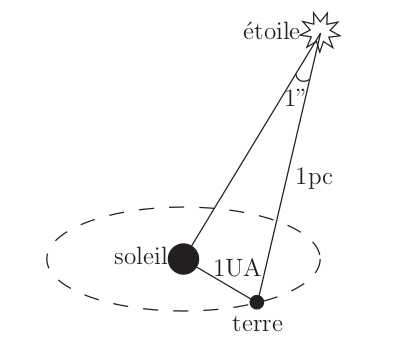
\includegraphics[width=15pc]{t1.png}
\caption{ Détermination des distance entre la terre- soleil- étoile en UA}
% \includegraphics[width=15pc]{w_t2.eps}
% \caption{}
\end{center}
\end{figure}
 
 
 \begin{align*}
 pc=\frac{1\text{UA}}{1\text{arcsec}} &\simeq \; 3,26 \; \text{ ly}\\
 & \simeq \; 3.10^{18}\text{cm}
 \end{align*} 
 
 $\qquad$ Notre Univers est homog\`ene et isotrope \`a grande \'echelle (i.e pour des \'echelles plus grandes que l'\'echelle des amas de galaxie). Homog\`ene signifie qu'il n'existe pas de point pr\'ef\'er\'e dans l'espace. Isotrope signifie qu'il n'existe pas de direction pr\'ef\'er\'ee. Pour montrer que l'Univers est isotrope, on peut observer le ciel dans diff\'erentes directions et compter le nombre de galaxies pour voir s'il est plus ou moins le m\^eme dans chaque direction. Une autre preuve pour l'isotropie de l'Univers vient du fond de rayonnement cosmique (CMB -" Cosmic Microwave Brackground") qu'on discutera plus en d\'etail dans ce cours. Montrer que l'Univers est homog\`ene s'av\`ere plus difficile, vu qu'on ne peut pas l'\'etudier d'un autre point de l'espace. pour \'etudier l'homog\'en\'eit\'e on essaie de mesurer les distances entre les galaxies et de reconstruire une image en 3D de notre Univers. \\
 
 $\qquad$ On aimerait maintenant comprendre comment d\'ecrire math\'ematiquement un espace homog\`ene et isotrope. Essayons donc de trouver quelles sont les m\'etriques qui d\'ecrivent un espace homog\`ene et isotrope. Pour r\'epondre \`a cette question, oublions pour l'instant le temps et concentrons-nous sur la partie spatiale de la m\'etrique :
 \begin{equation*}
 ds^2=\gamma_{ij}dx^idx^j, \;  \text{avec signature}\left(\gamma \right) =\left(+,+,+ \right) 
 \end{equation*} \\
 
 $\qquad$ la m\'etrique $\gamma_{ij}$ d\'etermine compl\`etement la g\'eom\'etrie de l'espace courbe et entre autre le tenseur de courbure de Riemann $R_{ijl}$. Rappelons les propri\'et\'es sym\'etrie de Riemann 
 \begin{eqnarray}
  R_{ijkl} &=& -R_{jikl}, \cr 
  R_{ijkl} &=& -R_{ijlk},\cr
  R_{ijkl} &=& R_{klij}.
 \end{eqnarray} 
 On va utiliser ces propri\'et\'es et exiger qu'il n'existe pas de point ou de direction pr\'ef\'er\'e pour d\'eterminer la structure de $R_{ijkl}$ dans un espace homog\`ene et isotrope.\\
 
 $\qquad$ Choisissons un syst\`eme de coordonn\'ees localement plat autour d'un point $\bar{x}$, i.e. $\gamma	_{ij}=\delta_{ij}$ et $\Gamma_{jk}^i = 0$. Alors, par les propri\'et\'es de sym\'etrie et pour avoir un espace sans direction pr\'ef\'er\'ee, on aura :
 \begin{equation}
 R_{ijkl}=\zeta \left[ \delta_{ik} \delta_{jl} - \delta_{il} \ {jk}\right],
 \end{equation} 
 Par contraction des indices on trouve successivement le tenseur de Ricci et la courbure scalaire 
 \begin{eqnarray}
 R_{ij}&=&2\gamma_{ij} \zeta \cr
 R&=&6\zeta
 \end{eqnarray}
 On distingue 3 types d'espace 
 $	\begin{cases}
 \zeta >0 :\text{coubure constante positive},\\
 \zeta =0 : \text{espace plat}, \\
 \zeta <0 : \text{coubure constante n\'egative}.
 \end{cases}$ 
  \subsection*{Cas $\zeta =0$} 
  On peut  choisir les coordonn\'ees cart\'esiennes : $\gamma_{ij}= \delta_{ij}$. Donc 
  \begin{equation}
  dl^2=dx^2+dy^2+dz^2
  \end{equation}
  \subsection*{Cas $\zeta>0$} 
  En trois dimensions, on conna\^{\i}t un exemple d'un  espace homog\`ene et isotrope \`a courbure constante positive: la $3$-sph\`ere, $S^3$ d\'efinie par $ \sum_{i=1}^{4}x_i^2=a^2$, o\`{u} $a$ est le rayon de la sph\`ere. L'\'el\'ement de distance est le m\^eme qu'en espace plat quadri-dimensionnel, \`a savoir:
  
   \begin{eqnarray}
   dl^2= dx_1^2+dx_2^2+dx_3^2+dx_4^2
   \end{eqnarray}
   Toutefois sur la $3$-sph\`ere on peut exprimer $dx_4$ en fonction des autres coordonn\'ees, 
   \begin{eqnarray}
   x_1dx_1+x_2dx_2+x_3dx_3+x_4dx_4 =0,
   \end{eqnarray}
   d'o\`{u} 
   \begin{eqnarray}
   dl^2= dx_1^2+dx_2^2+dx_3^2+ \frac{(x_1dx_1+x_2dx_2+x_3dx_3)^2}{a^2-x_1^2+x_2^2+x_3^2}. 
   \end{eqnarray}
   On aimerait encore \'ecrire la m\'etrique sous une forme simplifi\'ee. Introduisons des coordonn\'ees sph\'eriques $(r,\theta,\varphi) $ d\'efinies par 
  \begin{eqnarray}
   x_1&=&r\sin \theta \cos \varphi \cr
   x_2&=&r\sin \theta \sin \varphi \cr
   x_3=r\cos \theta 
   \end{eqnarray}
   On trouve alors que 
    \begin{eqnarray}
    dx_1^2+dx_2^2+dx_3^2=dr^2+r^2\left[ d\theta ^2 + \sin ^2 \theta d\varphi^2  \right],
    \end{eqnarray}
    et 
    \begin{eqnarray}
    x_1dx_1+x_2dx_2+x_3dx_3=rdr.
    \end{eqnarray}
    L'\'el\'ement de longueur est donn\'e par 
    \begin{eqnarray}
    dl^2&=& dr^2+r^2\left[ d\theta ^2 + \sin ^2 \theta d\varphi ^2 \right] + \frac{r^2dr^2}{a^2-r^2} \cr
    &=& \frac{a^2}{a^2-r^2} dr^2+ r^2 \left[ d \theta^2 + \sin^2 \theta^2 d  d\varphi ^2 \right] 
    \end{eqnarray}
 Posons $d\Omega ^2 := d \theta ^2 + \sin ^2 \theta d\varphi ^2$ et $\bar{r}:= \frac{r}{a}, $ 
 \begin{equation}
dl^2 =a^2 \left[ \frac{d \bar{r}^2}{1-\bar{r}^2} + \bar{r}^2 d \Omega^2 \right] . 
\end{equation}
 Le domaine de d\'efinition des variables est 
  \begin{eqnarray}
  &&0 \leq \bar{r} \leq 1, \cr
 && 0\leq \theta \leq \pi , \cr
 && 0 \leq \varphi \leq 2\pi.
  \end{eqnarray}
Remarquons encore que la courbure scalaire est donn\'ee par $\frac{1}{a^2}>0$.
  
  \subsection*{Cas $\zeta <0$} 
  On s'attend \`a ce que le r\'esultat soit identique \`a celui de la sph\`ere, mais o\`{u} on a remplac\'e $a^2 \mapsto -a^2$ pour avoir une courbure scalaire n\'egative. Ainsi, 
  \begin{eqnarray}
   dl^2&=& \frac{-a^2}{-a^2-r^2} dr^2 +r^2d\Omega ^2 \nonumber \cr
  &=& a^2\left[ \frac{d \bar{r}^2}{1+\bar{r}^2} + \bar{r}^2 d\Omega^2 \right] 
  \end{eqnarray}
 Le domaine de d\'efinition des variables variables est donn\'e par 
 \begin{eqnarray}
 &&0 \leq \bar{r} \leq \infty, \cr
 &&0 \leq \theta \leq \pi , \cr
 && 0 \leq \varphi <2\pi .
 \end{eqnarray}
 
  On peut r\'esumer les trois cas par la formule g\'en\'erale 
  \begin{equation}
  dl^2=a^2\left[ \frac{d\bar{r}^2}{1-k\bar{r}^2} + \bar{r}^2d\Omega^2\right], 
  \end{equation} 
  o\`{u} 
  $$ k= \begin{cases}
   +1& \qquad  \text{, Univers ferm\'e,} \\
   0 &\qquad \text{, espace plat} \\
   -1 &\qquad \text{, Univers ouvert.} 
   \end{cases}$$
   Notons qu'avec une red\'efinition des coordonn\'ees, on peut toujours se ramener \`a\\ $k=-1,0,1$. Ces trois valeurs de $k$ correspondent aux diff\'erentes g\'eom\'etries possibles. La terminologie d'un Univers ferm\'e ou ouvert se r\'ef\`ere \`a la finitude ou infinitude du volume de l'Univers. \\
   
   Finalement, on doit rajouter la composante temporelle. Si l'espace est homog\`ene et isotrope, le param\`etre d'\'echelle $a$ peut au plus d\'ependre du temps. Ainsi, 
   \begin{equation}
    ds^2 = dt^2 -a(t)^2 \left[ \frac{d\bar{r}^2}{1-k\bar{r}^2} +\bar{r}^2 d \Omega ^2\right] .
   \end{equation}
  Cette m\'etrique est appel\'ee m\'etrique de Robertson-Walker (RW). Ci-dessus nous donnons les composantes non nulles des symboles de Christofell et du tenseur de Ricci, ainsi que la courbure scalaire.  
  \begin{eqnarray}
   \Gamma _{ij}^0&= & \frac{\dot{a}}{a} g_{ij} \cr
   \Gamma_{0j}^i &=& \frac{\dot{a}}{a} \delta_j^i, \cr
   \Gamma_{jk}^i &=& \frac{1}{2} g^{il} \left[ \partial_k g_{lj} + \partial_j g_{lk} - \partial_l g_{jk}  \right] \cr
   R_{00}&=& -3 \frac{\ddot{a}}{a}, \cr
   R_{ij}&=& - \left[ \frac{\ddot{a}}{a}+ 2 \frac{\dot{a}^2}{a^2} +2ka^2 \right] g_{ij} , \cr
   R&=& -6 \left[ \frac{\ddot{a}}{a} + \frac{\dot{a}^2}{2} + \frac{k}{a^2} \right]  .   
 \end{eqnarray}
  \section{Equations de Friedman} 
  Nous allons maintenant d\'eriver les \'equations r\'egissant l'Univers lorsque celui-ci est d\'ecrit par la m\'etrique de Robertson-Walker. Pour ce faire nous utilisons les \'equtions d'Einstein en prenant comme mati\`ere un fluide parfait qui d\'ecrira notre Univers homog\`ene et isotrope. Le tenseur d'\'energie-implusion d'un fluide parfait est: 
  \begin{eqnarray}
  T_{\mu \nu }= (p+\rho )u_\mu u _\nu -pg_{\mu \nu }
  \end{eqnarray}
  o\`{u} $p$ est la pression, $\rho $ la densit\'e d'\'energie et $u^\mu $ le quadri-vecteur vitesse. Si le fluide est au repos $u^\mu=\{1, \overrightarrow{0}\} $, alors $T_{OO}= \rho $ et $T_{ij}= -pg_{ij}$. \\
  
  
  En injectant ceci dan les \'equations d'Einstein
  \begin{eqnarray}
  R_{\mu \nu} - \frac{1}{2} g_{\mu \nu }
   R- \lambda g_{\mu \nu } = 8 \pi G T_{\mu \nu }, 
   \end{eqnarray}
   on trouve pour la composante $\mu =\nu =0$: 
   \begin{eqnarray}
   -3 \frac{\ddot{a}}{a} -\frac{1}{2} (-6)
 \left[\frac{\ddot{a}}{a} + \frac{\dot{a}^2}{a^2} + \frac{k}{a^2} \right] - \lambda = 8 \pi G \rho,
 \end{eqnarray}
ce qui nous donne la premi\`ere \'equation de Friedmann
\begin{eqnarray}
\frac{\dot{a}^2}{a^2} + \frac{k}{a^2} - \frac{\lambda}{3} = \frac{8\pi G}{3} \rho .
\end{eqnarray}
Pour la composante $ij$ on trouve 

\begin{eqnarray}
- \left[ \frac{\ddot{a}}{a} +2 \frac{\dot{a}^2}{a^2} +2 \frac{k}{a^2} \right]  g_{ij}  - \frac{1}{2} (-6) \left[ \frac{\ddot{a}}{a} + \frac{\dot{a}^2}{a^2} + \frac{k}{a^2} \right] g_{ij} - \lambda g_{ij} =8 \pi G(-p) g_{ij} ,
\end{eqnarray}
ce qui nous donne la deuxi\`eme \'equation de Friedmann 
\begin{eqnarray} 
2 \frac{\ddot{a}}{a} + \frac{\dot{a}^2}{a^2} + \frac{k}{a^2}- \lambda = -8\pi Gp.
\end{eqnarray}
 
 Toutes  les autres composantes des \'equations d'Einstein sont identiquement nulles. Voici en r\'esum\'e les \'equations r\'egissant l'Univers homog\`ene et isotrope d\'ecrit par la m\'etrique de Robertson-Walker, que l'on appelle commun\'ement \'equations de Friedmann 
 \begin{eqnarray}
 \frac{\dot{a}^2}{\dot{a}^2} + \frac{k}{a^2} - \frac{\lambda }{3} & = \frac{8 \pi G }{3} \rho \\
 2 \frac{\ddot{a}}{a} + \frac{\dot{a}^2}{a^2} + \frac{k}{a^2} - \lambda &= -8 \pi G p.
 \end{eqnarray} 
\textbf{Conservation du tenseur d'\'energie-impulsion} 

Par ailleurs, on aura la conservation du tenseur d'\'energie-impulsion 
\begin{equation}
\nabla_\mu T^{\mu \nu } = \partial_\mu T^{\mu\nu } + \Gamma_{\mu \alpha } ^\mu T^{\alpha \nu } + \Gamma_{\mu \alpha } ^\nu T^{\mu \alpha } =0
\end{equation}
Un calcul explicite de la composante $\nu =0$ donne 
\begin{eqnarray}
\nabla_\mu T^{\mu 0} &= \partial_\mu T^{\mu 0} + \Gamma_{\mu \alpha } ^\mu T^{\alpha 0} + \Gamma_{\mu \alpha }^0 T^{\mu \alpha } = \partial_0 T^{00} + \Gamma_{\mu 0}^\mu T^{00} + \Gamma_{ij}^0T^{ij}  \nonumber\\
&= \dot{\rho} +3 \frac{\dot{a}}{a} \rho + \dot{a}a \delta_{ij} p \frac{1}{a^2} \delta{ij} = \dot{\rho} + 3 \frac{\dot{a}}{a}\left( \rho +p \right) \nonumber ,  
\end{eqnarray}
d'o\`{u} 
\begin{equation}
\dot{\rho} + 3 \frac{\dot{a}}{a} \left(\rho +p \right) =0
\end{equation} 
ce qui peut \^etre mis sous la forme suivante:
\begin{equation}
   \frac{\partial}{\partial t} \left[\rho a^3 \right] +p \frac{\partial }{\partial t} a^3 =0,
\end{equation} 
c'est \`a dire 
\begin{equation}
dE+pdV=0.
\end{equation}
Ceci n'est rien d'autre que la premi\`ere loi de thermodynamique. 
\textbf{Forme \'equivalente des \'equations de Friedmann} 
Introduisons les notations suivantes:
\begin{eqnarray}
  \rho_\lambda := \frac{\lambda}{8\pi G} , \qquad \qquad \rho_{tot} := \rho + \rho_\lambda , \nonumber\\
  p_\lambda := - \frac{\lambda }{8\pi G} , \qquad \qquad p_{tot} := p+p_\lambda \nonumber
\end{eqnarray}

Ce sont la densit\'e et la pression associ\'ees \`a la constante cosmologique ainsi que la densit\'e et pression  totale provenant de la mati\`ere et de la constante cosmologique. Avec ces notations, les \'equations de Friedmann peuvent \^etre r\'e\'ecrites de la mani\`ere suivante :
\begin{eqnarray}
\frac{\dot{a}^2}{a^2} + \frac{k}{a^2}&=\frac{8\pi G}{3} \rho_{tot},\\
2\frac{\ddot{a}}{a} + \frac{\dot{a}}{a^2} + \frac{k}{a^2}&=-8\pi G p_{{tot}}.
\end{eqnarray}
On peut \'eliminer k en prenant la diff\'erence de ces deux \'equations 
\begin{equation}
\frac{\ddot{a}}{a}=-\frac{4\pi G}{3}\left(\rho_{tot}+3p_{tot} \right) 
\end{equation} 
En tout on d\'eriv\'e quatre \'equations : deux \'equations de Friedmann, une \'equation provenant de la conservation de l'\'energie-impulsion et l'\'equation qu'on vient d'obtenir. Parmi ces \'equations, il n'y a que deux qui sont lin\'eairement ind\'ependantes. Selon la nature du probl\`eme il peut \^etre plus utile de travailler avec une \'equation plut\^ot qu'avec une autre.\\

\textbf{Param\`etre de d\'ec\'el\'eration } \\
On d\'efinit le param\`etre de d\'ec\'el\'eration $q$ par 
\begin{equation}
q\left(t \right) : = -\frac{\ddot{a}}{aH^2}=-\frac{\ddot{a}a}{\dot{a}^2},
\end{equation}
qu'on peut exprimer en fonction des param\`etres de densit\'e observables :
\begin{equation}
q\left(t \right) =-\frac{\ddot{a}}{aH^2}=\frac{4\pi G}{3} \frac{\rho _{tot} + 3 p_{tot}}{\frac{8 \pi G}{3} \rho_{tot} - \frac{k}{a^2}}.
\end{equation}
\text{	Dans le cas d'un Univers plat $k=0$, on obtient} 
\begin{eqnarray}
\Rightarrow q\left(t \right) = \frac{\rho_{tot}+3p_{tot}}{2\rho_{tot}} 
\end{eqnarray}
En explicitant les diff\'erentes contributions \`a l'\'energie et \`a la pression \\
\begin{eqnarray}
\rho_{tot}=\rho_{mat}+\rho_{rad}+\rho_\lambda , \qquad p_{tot} =p_{rad}+p_{\lambda} ,
\end{eqnarray}
on peut \'ecrire
\begin{equation}
q\left(t \right)=\frac{\Omega_{mat}}{2} + \frac{1+3w_\lambda}{2} \Omega_\lambda ,
\end{equation}
o\`{u} on a introduit $w_\lambda=\frac{p_\lambda}{\rho_\lambda }$ et les fractions critiques $\Omega$. Le premier terme du membre de droite est toujours positif, mais le second peut \^etre n\'egatif si $ 1+3 w_\lambda < 0$ .Donc si $w_\lambda<-1/3$ et si le deuxi\`eme terme est assez grand, le param\`etre  de d\'ec\'el\'eration peut prendre une valeur n\'egative. Il d\'ecrit alors un Univers en expansion acc\'el\'er\'ee, et on l'appelle alors parfois param\`etre d'acc\'el\'eration. Les observations de Supernovae de type la sont en faveur d'un $w_\lambda < - \frac{1}{3}$ et notre Univers se trouve actuellement en expansion acc\'el\'er\'ee.
\section{Diff\'erentes solutions des \'equations de Friedmann}

\textbf{Univers statique sans constante cosmologique $ \dot{a}=0, \lambda =0$} \\

Dans ce cas les \'equations de Friedmann se r\'eduisent \`a 
\begin{eqnarray}
 \frac{k}{a^2} & =& \frac{8\pi G}{3} \rho ,  \cr
 \frac{k}{a^2}&=& - 8 \pi G p.
\end{eqnarray}

 Comme l'Univers n'est pas vide, on a $\rho >0$, et la premi\`ere \'equation impliquerait alors que $k>0$. Mais pour $k=1$, la deuxi\`eme \'equation impliquerait que la pression serait n\'egative $p<0$, ce qui n'a pas de sens. On doit donc conclure qu'il n'existe pas de solution consistante pour un Univers statique sans constante cosmologique. 
 
 
 Historiquement, Einstein avait d\'ej\`a r\'ealis\'e ce probl\`eme. Comme il croyait en l'existence d'un Univers statique il d\'ecida en 1917 de rajouter une constante cosmologique non-nulle aux \'equations. En 1929, quand Hubble mettais en \'evidence l'expansion de l'Univers, Einstein revenait sur l'introduction de la constante cosmologique, la qualifiant de "plus grande b\^etise de sa vie" . Des observations r\'ecentes sugg\`erent qu'il existe n\'eanmoins une constante cosmologique non-nulle, mais tr\`es petite. A l'heure actuelle on ne sait pas expliquer pourquoi elle est si faible; c'est le probl\`eme de la constante cosmologique.  \\
 
 \textbf{Univers statique avec constante cosmologique : $\dot{a}=0 , \lambda \neq 0$} \\
 Les \'equations de Friedmann s'\'ecrivent 
 \begin{eqnarray}
  \frac{k}{a^2}- \frac{\lambda}{3} & = &\frac{8\pi G}{3} \rho . \cr
  \frac{k}{a^2} -\lambda &=& -8 \pi Gp. \nonumber
 \end{eqnarray}
  Si les vitesses des \'etoiles sont faibles, on peut supposer que $p\simeq 0$. La deuxi\`eme \'equation implique alors 
  \begin{equation}
  \frac{k}{a^2}= \lambda ,
  \end{equation} 
  ce qui, inject\'e dans la premi\`ere \'equation, nous donne 
  \begin{equation}
  \lambda = 4 \pi G \rho 
  \end{equation}
   Comme $\rho >0$ on doit aussi avoir $\lambda >0$ et donc $k>0$. Pour $k=1$ on trouve pour $a$: 
   \begin{equation}
   a=\frac{1}{\sqrt{\lambda}} = \frac{1}{\sqrt{4\pi G \rho}}
   \end{equation} 
  Cette relation entre la densit\'e $\rho $ et la taille de l'Univers f\^ut d\'ej\`a d\'eriv\'ee par Einstein en 1917. Ce mod\`ele statique d'Einstein a malheureusement un probl\`eme conceptuel : si on suppose $\rho =0$, alors comme $\lambda \neq 0$, l'espace vide lui-m\^eme engendrerai une force de gravitation.\\
  \textbf{Univers vide statique: $\dot{a}=0 , \rho = p=0$} \\
  Les \'equations de Friedmann se r\'eduisent \`a : 
  \begin{eqnarray}
  \frac{k}{a^2} - \frac{\lambda}{3}& =&0 , \cr
  \frac{k}{a^2} - \lambda &=0&. 
  \end{eqnarray}
  On est alors confront\'e  au paradoxe suivant : si $\lambda =0$, alors $k=0$ et un Univers plat est donc solution. Mais on sait que dans ce cas il n'existe pas de solution statique. Pour avoir une solution statique il faut choisir $\lambda \neq 0$, donc $k \neq 0$ mais alors l'espace plat n'est plus une solution. Ce paradoxe f\^ut r\'esolu en 1922 quand Alexander Friedmann proposait un mod\`ele dans lequel l'Univers n'est plus statique.
  
  \textbf{Univers non-statique: $ \dot{a} \neq 0$} 
  
  Consid\'erons, pour simplifier, un Univers plat sans constante cosmologique:  $\lambda = k=0$.
  Les \'equations de Friedmann sont alors 
  \begin{eqnarray}
  \frac{\dot{a}^2}{a^2} & = &\frac{8\pi G}{3} \rho , \cr
  2 \frac{\ddot{a}}{a} + \frac{\dot{a}^2}{a^2} & =&-8 \pi G p\simeq 0. 
  \end{eqnarray}
  Multiplions la deuxi\`eme \'equation par $\frac{a}{\dot{a}}$ 
  \begin{eqnarray}
  && \implies 2 \frac{\ddot{a}}{\dot{a}} + \frac{\dot{a}}{a} =0 \implies \frac{d}{dt}
  \left( 2 \ln \dot{a} + \ln a \right)  =0 \cr
  && \implies \ln \left( \dot{a}^2a \right) = \text{ const } \implies \dot{a}^2a = \text{ const } \cr
  &&\implies \sqrt{a}da = \text{ const } . \; dt \implies a^{3/2} =\text{ const }.t.    
  \end{eqnarray} 
   D'o\`{u} 
   \begin{equation}
   a(t) = a_0 \left( \frac{t}{t_0} \right) ^{2/3}
   \end{equation} 
   On voit que $a$ augmente en fonction du temps- l'Univers est en expansion. On peut ensuite injecter cette solution dans la premi\`ere \'equation de Friedmann : 
   \begin{eqnarray}
   &  \implies \left( \frac{2}{3} \frac{1}{t} \right) = \frac{8\pi G}{3} \rho , \nonumber \\
   & \implies \rho = \frac{4}{9} \frac{3}{8 \pi G} \frac{1}{t^2}.
   \end{eqnarray}
   D'o\`{u} 
   \begin{equation}
   \rho (t) = \frac{1}{6 \pi G} \frac{1}{t^2}.
   \end{equation}
   
   En particulier, connaissant la densit\'e $\rho$, on peut d\'eterminer l'\^{a}ge de l'Univers. Constatons aussi que pour $t \rightarrow 0 $, la densit\'e diverge $\rho \rightarrow \infty $ (Big Bang). 
  
 \section{Equations de Friedmann en m\'ecanique Newtonienne} 
 
 Il s'av\`ere que l'on peut d\'eriver l'essentiel des \'equations de Friedmann d\'ej\`a en m\'ecanique Newtonienne et sans avoir recours \`a la relativit\'e g\'en\'erale. Consid\'erons le cas suivant 
  	$ k=0$, espace plat , 
  	$\lambda =0 $ , le vide ne produit pas de force gravitationnelle, 
  	$  p=0$, mouvement non-relativiste $(p<< \rho ). $ 
Consid\'erons une sph\`ere de rayon variable $a(t)$ remplie d'un gaz de particules sans interaction distribu\'ees de fa\c con homog\`ene et isotrope. D'une part on peut \'ecrire la conservation de l'\'energie totale \`a l'int\'erieur de cette sph\`ere :
 \begin{equation}
\frac{d}{dt}\left(  \frac{4}{3} \pi a^3 . \rho  \right) =0 
 \end{equation} 
 En d\'eveloppant on retrouve une des \'equations de Friedmann : 
 \begin{equation}
 \dot{\rho} + 3 \frac{\dot{a}}{a} \rho =0. 
 \end{equation}
 D'autre part on peut \'ecrire la loi de Newton pour une particule de gaz de masse $m$ situ\'ee sur la sph\`ere :
 \begin{equation}
 m \ddot{a} = -G . \frac{4}{3} \pi a^3 \rho .m. \frac{1}{a^2}
 \end{equation}
  Ce qui implique 
  \begin{equation}
  \frac{\ddot{a}}{a} = - \frac{4 \pi G}{3} \rho 
  \end{equation} 
  On a retrouv\'e l'autre \'equation de Friedmann dans le cas particulier $p_{tot} =0$ et $\rho_{tot}=\rho $. Pour trouver le terme $+3 p_{tot}$ dans cette \'equation il faut utiliser la relativit\'e g\'en\'erale.
  \section{Propagation de la lumi\`ere dans l'Univers- D\'ecalage vers le rouge}  
  On aimerait \'etudier la propagation de la lumi\`ere dans un Univers d\'ecrit par les \'equations de Friedmann. Le moyen direct serait d'\'etudier les \'equations de Maxwell dans l'espace courbe de Robertson-Walker. Mais il y a en fait un moyen plus facile qui est de faire usage d'un syst\`eme de coordonn\'ees particulier, appelle coordonn\'ees conformes. On r\'e\'ecrit la m\'etrique de Robertson-Walker comme suit 
  \begin{eqnarray}
  ds^2 & =& dt^2 + a^2(t) dl^2 \cr
  &= &a^2(t) \left[ \frac{dt^2}{a^2(t)} +dl^2 \right]   
  \end{eqnarray} 
  On introduit le temps conforme $\eta $ d\'efinit par 
  \begin{equation}
  d\eta := \frac{dt}{a(t)},
  \end{equation} 
  donc 
  \begin{equation}
  \eta - \eta_0 = \int_{0}^{t} dt^\prime \frac{1}{a(t^\prime)} 
  \end{equation}
  La m\'etrique s'\'ecrit alors 
  \begin{equation}
  ds^2 = a^2(\eta) \left[ d\eta ^2 +dl^2 \right] \equiv a^2(\eta) \bar{g}_{\mu \nu } dx^\mu dx^ \nu.
  \end{equation}
  La m\'etrique $\bar{g}_{\mu \nu} $ ainsi d\'efinie est ind\'ependante du temps. On peut maintenant \'etudier les \'equations de Maxwell dans ce syst\`eme de coordonn\'ees. Nous allons partir de l'action de l'\'electromagn\'etisme dans un espace courbe 
  \begin{eqnarray}
  S_{EM} = \displaystyle \int d^4 x \sqrt{|g|}
  \left[ - \frac{1}{4} g^{\mu \nu } g^{\rho \sigma } F_{\mu  \rho } F_{\nu \sigma } \right]. 
  \end{eqnarray}
  Pour le syst\`eme de coordonn\'ees de temps conforme on a 
  \begin{eqnarray}
   \sqrt{|g|} = \sqrt{\left[ a^2(\eta) \right]^4  } \sqrt{|\bar{g}|} =a^4 (\eta ) \sqrt{|\bar{g}|}, 
   \end{eqnarray}
   et 
   \begin{eqnarray}
   g^{\mu \nu } = \frac{1}{a^2(\eta )} \bar{g}^{\mu \nu } 
   \end{eqnarray}  
   D'o\`{u} 
   \begin{eqnarray}
   S_{EM} - \frac{1}{4} \displaystyle \int d^4x a^4(\eta) \sqrt{|\bar{g}|}. \frac{1}{a^2(\eta)} \bar{g}^{\mu \nu} . \frac{1}{a^2(\eta)} \bar{g}^{\rho \sigma } . F_{\mu \rho } F_{\nu \sigma}, 
   \end{eqnarray}
   ou encore 
   \begin{equation}
   S_{EM} = - \frac{1}{4} \displaystyle \int d^4x \sqrt{|\bar{g}|} \bar{g}^{\mu \nu } \bar{g}^{\rho \sigma } F_{\mu \rho } F_{\nu \sigma } 
   \end{equation}
   Comme $\bar{g}_{\mu \nu }$ est statique, cette action ne d\'epend pas explicitement du temps. De plus, si on consid\`ere des "petites" distances $(\bar{r}<<1)$, on peut supposer que l'espace est pratiquement plat $(k=0)$ et utiliser pour $\bar{g}_{\mu \nu }$ la m\'etrique de Minkowski: 
   \begin{eqnarray}
   ds^2 \simeq a^2 ( \eta) \eta_{\mu \nu } dx^\mu dx^\nu.
   \end{eqnarray}
   Dans ce cas, les solutions des \'equations de Maxwell sont simplement des ondes planes 
   \begin{equation}
   A_\mu \propto \mathrm{e}^{i \omega \eta +ik \bar{x}},
   \end{equation} 
   o\`{u} $\omega , k = \text{const} $ et $ \bar{x}, \eta , \omega , k $ sont sans dimension. 
   
   Ayant trouv\'e la solution des \'equations de Maxwell, on doit encore l'interpr\'eter physiquement. Rappelons qu'on a utilis\'e les coordonn\'ees suivantes 
   \begin{eqnarray}
   ds^2 =a^2(\eta ) \left[ d \eta ^2 -d\bar{x}^2 \right]   
   \end{eqnarray}
   
      	Un observateur de cette onde \'electromagn\'etique utilisera simplement la m\'etrique de Minkowski
      	\begin{eqnarray}
      	ds^2=dt^2-dx^2
      	\end{eqnarray}
      	On obtient ainsi la relation 
      	\begin{eqnarray}
      	a^2\left(\eta \right)d\bar{x}^2=dx^2. 
      	\end{eqnarray}
      	Ainsi l'observateur va en fait observer une onde plane donn\'ee par
      	\begin{eqnarray}
      	A_\mu \propto e^{iw\eta +ik\frac{x}{a\left(\eta \right) }}
      	\end{eqnarray}
      	Cet observateur va donc mesurer comme longueur d'onde 
      	\begin{equation}
      	\lambda = \frac{2\pi a\left(t \right) }{k}
      	\end{equation}
      	On conclut que $\lambda\propto a\left( t \right) $. Dans un Univers en expansion, le facteur d'\'echelle $a \left(t \right)$ croit, et donc aussi la longueur d'onde de la lumi\`ere observ\'ee. On peut illustrer cette augmentation de la longueur d'onde en s'imaginant de dessiner une onde sur un ballon et de le gonfler; la longueur va augmenter  avec le rayon du ballon.	
      	
      	
      	
      	
\begin{figure}[h]
\begin{center}
	%\begin{minipage}{14pc}
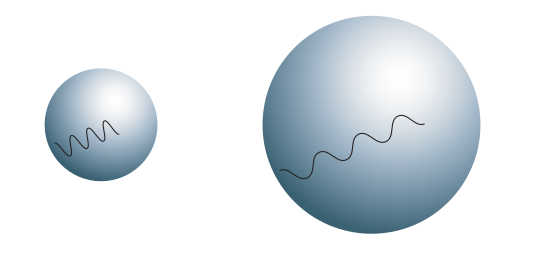
\includegraphics[width=15pc]{t2.png}
\caption{Augmentation de la longueur d'onde \`a cause de l'expansion de l'Univers}
% \includegraphics[width=15pc]{w_t2.eps}
% \caption{}
\end{center}
\end{figure}
      	\qquad Consid\'erons une source lumineuse (e.g.\'etoile) \'emettant de la lumi\`ere de longueur d'onde $\lambda_0$ \`a une distance $l$ de la terre. Calculons la longueur d'onde $\lambda$ qu'on observerait sur la terre. Soit $t$ le temps de r\'eception du signal sur terre et soit $t_0\simeq t-\frac{l}{c}$ le temps d'\'emission du signal lumineux (cette relation n'est qu'approximative car l'Univers est en expansion). Comme $\lambda \propto a$ on a 
      	\begin{eqnarray}
      	\frac{\lambda_0}{\lambda}=\frac{a\left( t_0\right) }{a\left(t \right) }\Rightarrow \lambda\left( t\right) =\lambda_0 \frac{a\left( t\right) }{a\left( t-\frac{l}{c}\right) }
      	\end{eqnarray}
      	Comme $\frac{l}{c}$ est petit, on peut d\'evelopper en s\'erie 
      	\begin{eqnarray}
      	\lambda\left( t\right) \simeq\lambda_0 \frac{a\left( t\right) }{a\left( t\right) \left( t-\frac{l}{c}\right) } \simeq \lambda_0\left(1+\frac{\dot{a}}{a} \frac{l}{c} \right) 
      	\end{eqnarray}
      	
      	On appelle d\'ecalage vers le rouge ("redshift"), not\'e $z$, le rapport 
      	\begin{equation}
      	z:= \frac{\lambda- \lambda_0}{\lambda_0} \\
      	\end{equation}
      	D'o\`{u} finalement (avec $c=1$)
      	\begin{equation}
      	z=\frac{\dot{a}}{a}l= Hl,
      	\end{equation}
      	o\`{u} $H:=\frac{\dot{a}}{a}$ est appel\'e constante de Hubble, m\^{e}me si elle n'est  pas vraiment une $constante $ vu qu'elle d\'epend du temps. On note par $H_0$ la constante de Hubble \`a notre \'epoque, donc $H_0=H\left(t_0 \right) $. La relation entre le d\'ecalage vers le rouge et la constante de Hubble est commun\'ement appel\'ee la loi de Hubble. Elle montre que, dans un Univers en expansion, les longueurs d'ondes sont d\'eplac\'ees vers le rouge . En 1929, Edwin Hubble a observ\'e en premier cette relation lin\'eaire entre la distance $l$ et le d\'ecalage vers le rouge $z$. C'\'etait une premi\`ere indication exp\'erimentale pour l'expansion de l'Univers. Ci- apr\`es se trouvent deux diagrammes de Hubble. Ils montrent la vitesse de la source en fonction de sa distance. Surtout le diagramme r\'ecent de 2005 met bien en \'evidence une d\'ependance lin\'eaire. Actuellement, les mesures du param\`etre de Hubble donnent  :
      	\begin{equation}
      	H_0= 71 \pm \frac{km/s}{Mpc}
      	\end{equation}
      	
%       \begin{figure}[h]
% %\begin{minipage}{14pc}
% 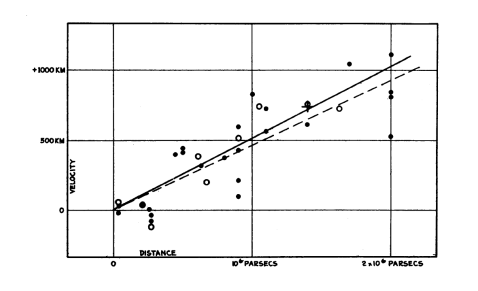
\includegraphics[width=15pc]{t3.png}
% \caption{Diagramme publi\'e par Edwin
% Hubble dans son article de $1929$ \cite{1}}
%  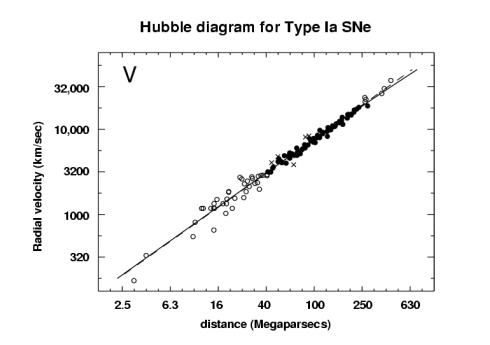
\includegraphics[width=15pc]{t4.png}
%  \caption{Diagramme de Hubble (pour
% les supernovae) de $2005$ \cite{2}}
% \end{figure}
      	
      	 \begin{figure}[h]
\begin{center}
	\begin{minipage}{14pc}
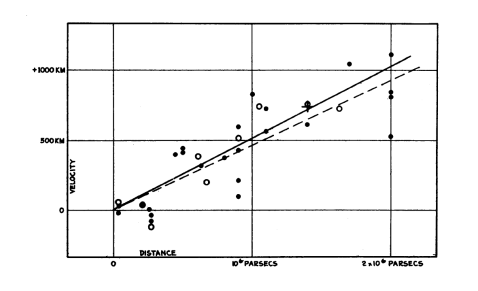
\includegraphics[width=15pc]{t3.png}
\caption{Diagramme publi\'e par Edwin
Hubble dans son article de $1929$ \cite{1}}
\end{minipage}\hspace{3pc}%
\begin{minipage}{14pc}
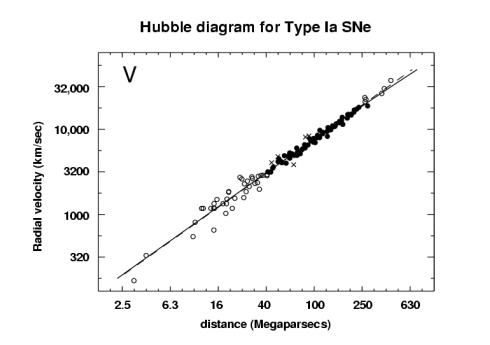
\includegraphics[width=15pc]{t4.png}
 \caption{Diagramme de Hubble (pour
les supernovae) de $2005$ \cite{2}}
 \end{minipage}\hspace{3pc}%
\end{center}
\end{figure}
      	
      	
      	On peut constater dans le diagramme de Hubble de 1929 que l'unit\'e pour la vitesse est fausse (km au lieu km/s). En plus, la valeur pour la constante $H_0$ d\'etermin\'ee par Hubble lui-m\^{e}me \'etait fausse d'un facteur $\sim 10$.
      	
      	
      	\qquad Exp\'erimentalement il est relativement ais\'e de mesurer le d\'ecalage vers le rouge des \'etoiles. Pour cela il suffit de mesurer le d\'eplacement des lignes spectrales dans le spectre de la lumi\`ere re\c{c}ue. La mesure des distances par contre est plus d\'elicates. L'id\'ee est de d\'eduire la distance de l'objet \`a partir de la luminosit\'e. Mais pour cela il faut faire usage de ce qu'on appelle des chandelles standards, qui est un d'objet astrophysique \`a luminosit\'e connue. Il est alors facile de relier la luminosit\'e de ces chandelles standards et la luminosit\'e observ\'ee sur terre \`a leur distance.\\
      	
      	$\qquad$ Il existe une interpr\'etation \'equivalente de la loi de Hubble \`a l'aide de l'effet Doppler. On consid\`ere que l'observateur est au repos, mais que la source s'\'eloigne de lui \`a ue vitesse $v$. Alors, par effet Doppler, la longueur d'onde observ\'ee sera diff\'erente de celle \'emise  plus particuli\`erement on aura :
      	\begin{eqnarray}
z=\sqrt{\frac{1+v}{1-v}}-1 \overset{v<<c}{\simeq} v = \dot{l} = \frac{\dot{a}}{a} l, 
\end{eqnarray}
      	c'est \`a dire
     	\begin{eqnarray} 
     	\dot{\overrightarrow{l}} =H \overrightarrow{l}.
     	\end{eqnarray}
      	Cette relation motive aussi le choix d'unit\'es pour la constante de Hubble :
      	\begin{equation}
      	[H]=\frac{[\dot{l}]}{[l]}= \frac{km/s}{Mpc}
      	\end{equation} 
      	$\qquad$ On a vu que l'homog\'en\'eit\'e et l'isotropie de l'Univers impliquent la loi de Hubble. \'{E}tudions si la r\'eciproque est vraie aussi. Il est clair que la loi de Hubble implique que l'Univers est isotrope, vu que $H$ ne d\'epend pas de la direction d'observation. Il s'av\`ere que la loi de Hubble implique aussi que l'Univers est homog\`ene.
      	En effet, on a 
      	
      	     \begin{figure}[h]
\begin{center}
	%\begin{minipage}{14pc}
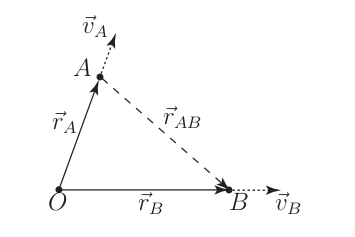
\includegraphics[width=15pc]{t5.png}
\caption{Mise en oeuvre de l'homogénéité de l'Univers grace à la relation de Hubble}
%  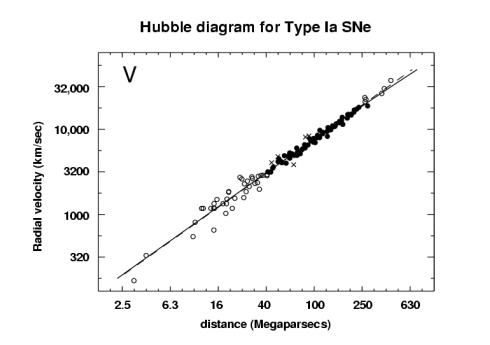
\includegraphics[width=15pc]{t4.png}
%  \caption{Diagramme de Hubble (pour
% les supernovae) de 2005 [2]}
\end{center}
\end{figure}
      	
      	mais aussi pour la vitesse du point $B$ par rapport au point $A$
      	\begin{eqnarray}
      	v_B ) _A &=&H\vec{r}_{AB} ,\cr
      	v_B ) _A &= &\vec{v}_B - \vec{v}_A =H\left( \vec{r}_B - \vec{r}_A\right). 
      	\end{eqnarray}
      	Les deux derni\`eres \'etant \'egales, on conclut qu'il y a homog\'en\'eit\'e.
    \section{Horizons} 
    
    L'Univers ayant un \^{a}ge fini, la lumi\`ere dans l'univers n'a p\^u parcourir qu'une distance finie. Il s'en suit que tr\`es probablement nous ne pouvons observer qu'une partie de notre Univers. De plus, si l'expansion de l'Univers est trop grande, cette partie visible d\'evient de plus en plus petite, vu que la lumi\`ere des r\'egions les plus lointaines ne peut plus nous atteindre. Pour discuter ces ph\'enom\`enes nous allons maintenant introduire la notion d'horizon. 

    \textbf{Horizon d'\'ev\`enement} 
    
     Le premier horizon  que nous introduisons est l'horizon d'\'ev\`enement ("event horizon"). Il correspond au rayon de la r\'egion de l'Univers dans le pass\'e qui peut nous influencer causalement. Tout \'ev\`enement en dehors de cet horizon ne peut pas nous influencer vu que seuls les signaux dans notre horizon d'\'ev\`enement peuvent nous atteindre. 
     
     
     Nous voulons calculer la distance qu'un photon peut parcourir s'il est \'emis \`a l'instant $t$. Supposons que le mouvement du photon se situe dans un plan et posons en cons\'equence dans la m\'etrique de Robertson-Walker $ds^2 =0 , d\theta =d \phi =0$, ce qui donne 
     \begin{eqnarray}
     \frac{dt}{a} = \frac{dr}{\sqrt{1-kr^2}} 
     \end{eqnarray}
     La distance en coordonn\'ees comobiles est alors donn\'ee par 
     \begin{eqnarray}
     D_e(t) = \displaystyle \int_{t}^{t_0} \frac{dt^\prime }{a(t^\prime )}. 
     \end{eqnarray}
 Pour passer \`a une distance physique il suffit de multiplier la distance exprim\'ee en coordonn\'ees comobiles par le facteur d'\'echelle : 
 \begin{eqnarray}
 d_e(t) =a(t) \displaystyle \int_{t}^{t_0} \frac{dt^\prime }{a(t^\prime )}.
 \end{eqnarray}
 Remarquons encore que toutes ces formules n'ont de sens que si les int\'egrales convergent. Si tel n'est pas le cas, on dit que l'horizon en question n'existe pas. 
 
 \textbf{Horizon de particule}  
 
 Le second horizon est appel\'e horizon de particule ("particle horizon"). Il s'agit de conna\^{\i}tre l'\'etendue de la r\'egion \`a laquelle nous sommes causalement reli\'es \`a l'instant $t_0$. En coordonn\'ees comobiles nous aurons 
 
 \begin{eqnarray}
 D_p(t_0) = \displaystyle \int_{t_{min}}^{t_0} \frac{dt}{a(t) }, 
 \end{eqnarray}

 et donc la distance physique est 
 \begin{eqnarray}
 d_p (t_0) =a(t_0) \displaystyle \int_{t_{min}}^{t_0} \frac{dt}{a(t)}.
 \end{eqnarray}

%      \begin{figure}[h]
% %\begin{minipage}{14pc}
% 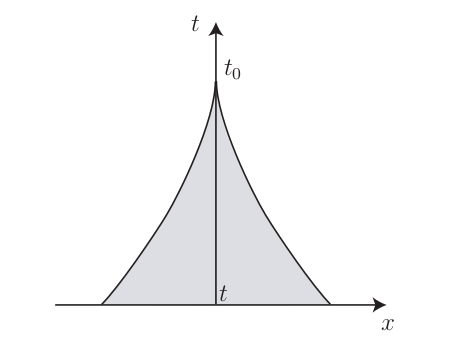
\includegraphics[width=15pc]{t6.png}
% \caption{Horizon d'\'ev\'enement}
%  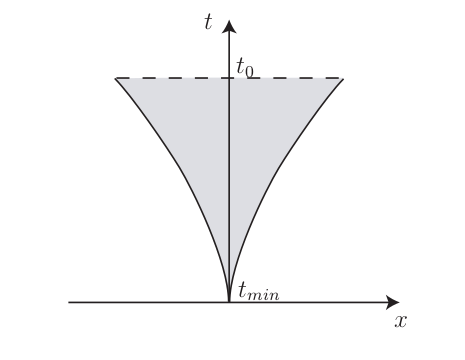
\includegraphics[width=15pc]{t8.png}
%  \caption{Horizon de particule}
% \end{figure}


\begin{figure}[h]
\begin{center}
	\begin{minipage}{14pc}
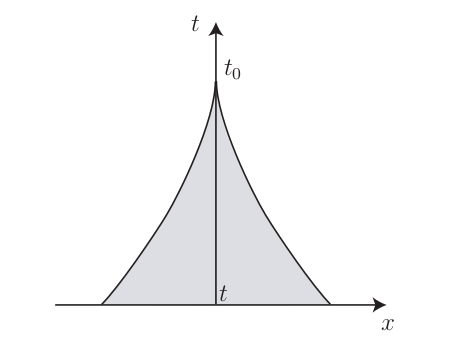
\includegraphics[width=15pc]{t6.png}
\caption{Horizon d'\'ev\'enement}
\end{minipage}\hspace{3pc}%
\begin{minipage}{14pc}
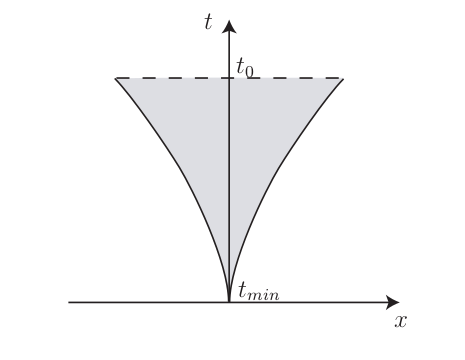
\includegraphics[width=15pc]{t8.png}
\caption{Horizon de particule}
\end{minipage}\hspace{3pc}%
\end{center}
\end{figure}

\section{Densit\'e critique de l'Univers} 


  Jusqu'\`a pr\'esent notre \'etude s'est limit\'ee au cas particulier $ \lambda =0 , p=0 , k=0$.  Afin de pouvoir faire une \'etude plus g\'en\'erale, commen\c cons par r\'e\'ecrire une des \'equations de Friedmann: 
  \begin{eqnarray}
  H^2 + \frac{k}{a^2} &=& \frac{8 \pi G}{3} \rho_{tot} \cr
  \implies \frac{k}{H^2a^2} &= &\frac{8\pi G \rho_{tot}}{3H^2} -1 \equiv \frac{\rho_{tot}-\rho_c}{\rho_c} 
  \end{eqnarray}   
  o\`{u} on a introduit la densit\'e critique d\'efinie par 
  \begin{equation}
  \rho_c := \frac{3H^2}{8\pi G} .
  \end{equation}
  La densit\'e critique peut \^etre d\'eduite de la constante de Hubble: 
  
  \begin{eqnarray}
  \rho_c \approx 1,88.h^2.10^{-29} \frac{g}{cm^3},
  \end{eqnarray}

  o\`{u} on a \'ecrit la constante de Hubble de la mani\`ere suivante 
  \begin{eqnarray} 
  H =100.h. \frac{km/s}{Mpc}
  \end{eqnarray}

  De plus, l'\'equation de Friedmann implique 
  \begin{equation}\label{31}
  sign(k)= sign(\rho_{tot}-\rho_c),
  \end{equation}
  ainsi 
 \begin{eqnarray}
  &&\rho_{tot} > \rho_c \implies k=1 \qquad \text{ Univers ferm\'e, } \cr
  &&\rho_{tot} = \rho_c \implies k=0 \qquad \text{ Univers plat, } \cr
  &&\rho_{tot} < \rho_c \implies k=-1 \qquad  \text{ Univers ouvert } 
  \end{eqnarray}
  La densit\'e critique n'est pas forc\'ement constante et peut d\'ependre du temps. Mais d'apr\`es  \ref{31} le signe de $\rho_{tot}-\rho_c$ est ind\'ependant du temps>. Les observations r\'ecentes sugg\`erent que 
  \begin{eqnarray}
  \rho_{tot} \simeq \rho_c \pm (2-3)  \% 
  \end{eqnarray}
  notre Univers est donc extr\^emement proche d'un Univers plat. 
  
  Il est utile d'introduire encore une autre notation ; les abondances $\Omega $, aussi appel\'ees les fractions critiques: 
  \begin{equation}
  \Omega_{mat} := \frac{\rho_{mat}}{\rho_c} , \; \Omega_\lambda 
  := \frac{\rho_\lambda }{\rho_c} , \; \Omega_k := - \frac{k^2}{a_0^2H_0^2}
  \end{equation}  
  
  Dans ces notations, l'\'equation de Friedmann prend une forme particuli\`erement simple 
  \begin{equation}
  \Omega_{mat} + \Omega_\lambda +\Omega_k =1.
  \end{equation} 
  \section{Le futur de l'Univers}
  On a vu que notre Univers se trouve dans un \'etat d'expansion. Mais que peut-on dire sur le futur de l'Univers? Consid\'erons la situation $ \lambda =0 , p=0$. La valeur de $k$ n'\'etant pas fix\'ee, prenons la forme des \'equations de Friedmann qui est ind\'ependante de $k$ 
  \begin{eqnarray} 
  \frac{\ddot{a}}{a} = - \frac{4 \pi G}{3} \rho ,
  \end{eqnarray}

  et multiplions par $a \dot{a} $ 
  \begin{equation}\label{34}
  \dot{a} \ddot{a} = \frac{1}{2} \frac{d}{dt} (\dot{a}^2) = - \frac{4\pi G}{3} \rho a \dot{a} 
  \end{equation}
 On aimerait r\'e\'ecrire $\rho a \dot{a}$ comme d\'eriv\'ee totale par rapport au temps. Pour cela, constatons d\'ej\`a qu'on a trivialement 
 \begin{equation}
 \frac{d}{dt} (\rho a^2)  = -3\rho a \dot{a} +2 \rho a \dot{a} =-\rho a\dot{a}
 \end{equation} 
 On peut \`a pr\'esent r\'e\'ecrire l'\'equation  \ref{34} comme d\'eriv\'ee totale et l'int\'egrer par rapport au temps:
 \begin{eqnarray}
 \frac{1}{2} \frac{d}{dt} (\dot{a}^2) = \frac{4\pi G}{3} \frac{d}{dt} (\rho a^2)
 \end{eqnarray}
  
 \begin{eqnarray}
 && \implies \frac{d}{dt} \left( \frac{1}{2} \dot{a}^2 - \frac{4 \pi G}{3} \rho a^2 \right)=0 \cr
 & &\implies \frac{1}{2} \dot{a}^2 - \frac{4\pi G}{3} \rho a^2 = \text{ const } \overset{t=t_0}{=} \frac{1}{2} \ddot{a}_0^2 - \frac{4 \pi G}{3} \rho_0 a_0^2  
 \end{eqnarray}
 De plus 
 \begin{eqnarray}
 \rho a^3 = \text{ const } &= &\rho_0 a_0^3 \implies \rho a^2 = \frac{\rho_0 a_0^3}{a} \cr
  H_0& =& \frac{\dot{a_0}}{a_0} \implies \dot{a}_0^2 H_0^2a_0^2,
 \end{eqnarray} 
 ce qui, inject\'e dans l'\'equation d'avant donne 
 \begin{eqnarray}
 \implies \dot{a}^2 &=& \frac{ 8 \pi G}{3} \frac{\rho_0 a_0^3}{a} + H_0^2 a_0^2 - \frac{ 4 \pi G }{3} \rho_0 a_0^2 \cr
 \implies \dot{a}^2 &=& \frac{8 \pi G }{3} \frac{\rho_0 a_0^3}{a} -  \frac{4 \pi G}{3} a_0^2 (\rho_0 -\rho_{c,0}) 
 \end{eqnarray}
 L'\'equation \`a r\'esoudre est donc 
 \begin{equation}
 \dot{a}^2 - \frac{8\pi G }{3} \frac{\rho_0 a_0^3}{a} =
 - \frac{4 \pi G}{3} a_0^2 (\rho_0 - \rho_{c,0})= \text{ const },
 \end{equation} 
 qui est clairement de la forme $E_{ein} +U =E_{tot} \text{ const } $. La solution exacte de cette \'equation est donn\'ee par : 
 \begin{equation}
 t =\pm  \displaystyle \int \frac{da}{\sqrt{\frac{ 8 \pi G}{3} \frac{\rho_0 a_0^3}{a} -
 \frac{4 \pi G }{3} a_0^2 (\rho_0 -\rho_{c,0})}}.
 \end{equation}
 Essayons de comprendre qualitativement les solutions en utilisant l'analogie avec la m\'ecanique classique. 
 
%       \begin{figure}[h]
% %\begin{minipage}{14pc}
% 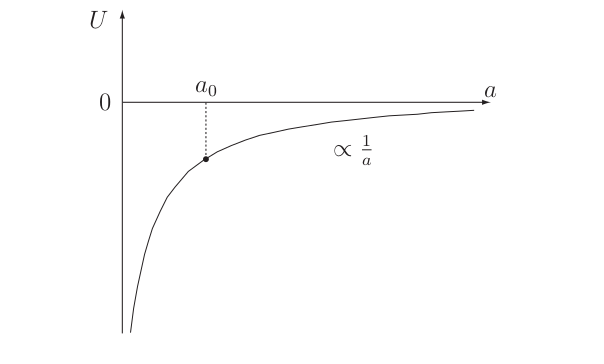
\includegraphics[width=15pc]{t9.png}
% \caption{Le potentiel en fonction de $a$.}
% %  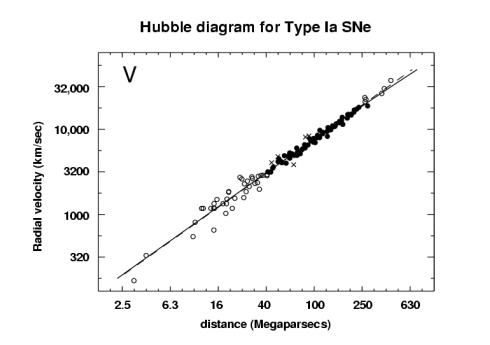
\includegraphics[width=15pc]{t4.png}
% %  \caption{Diagramme de Hubble (pour
% % les supernovae) de 2005 [2]}
% \end{figure}
 \begin{figure}[h]
\begin{center}
	\begin{minipage}{14pc}
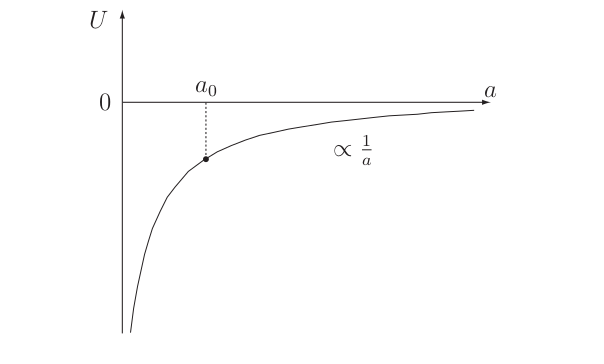
\includegraphics[width=15pc]{t9.png}
\caption{Evolution du potentiel en fonction de $a$.}
\end{minipage}\hspace{3pc}%
% \begin{minipage}{14pc}
% 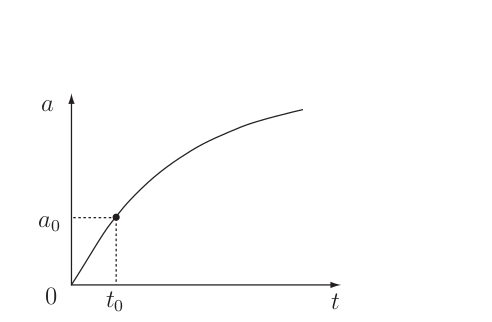
\includegraphics[width=15pc]{t13.png}
% \caption{}
% \end{minipage}\hspace{3pc}%
\end{center}
\end{figure}

%  
Il faut distinguer les cas suivants: 
\begin{enumerate}
	\item[i)] $\rho_0 =\rho_{c,0}$ , i.e. $E_{tot}=0:$ \\

	Dans ce cas la solution est simple et on l'a d\'ej\`a trouv\'e avant : $a \sim t^{2/3}$, \\$\implies $ expansion infinie. 
	\item[ii)] $\rho_0 > \rho_{c,0} $, i.e. $E_{tot} <0$:\\
	$a_{\max} = \frac{2a_0 \rho_0}{\rho_0 - \rho_{c,0}}$ 
	
% 	  \begin{figure}[h]
% %\begin{minipage}{14pc}
% 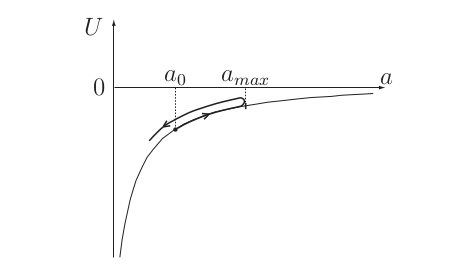
\includegraphics[width=15pc]{t10.png}
% \caption{}
%   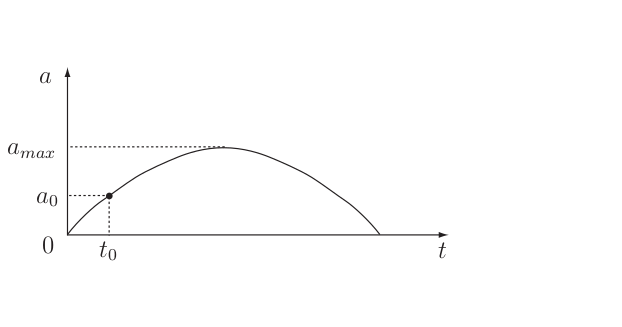
\includegraphics[width=15pc]{t11.png}
%   \caption{}
% \end{figure}
	
	\begin{figure}[h]
\begin{minipage}{14pc}
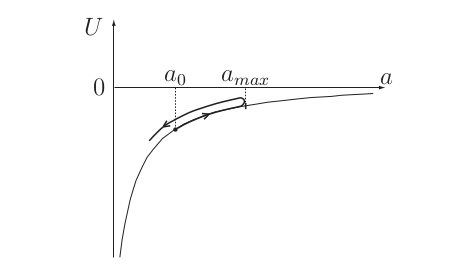
\includegraphics[width=15pc]{t10.png}
\caption{}
\end{minipage}\hspace{3pc}%
\begin{minipage}{14pc}
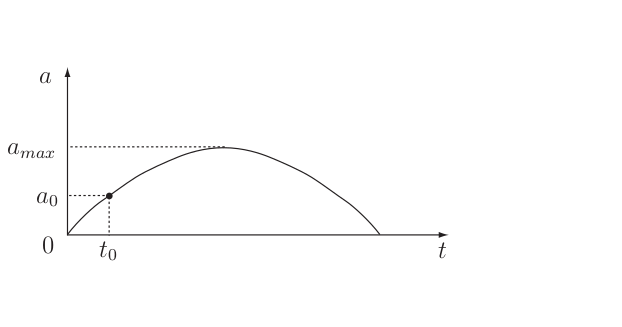
\includegraphics[width=15pc]{t11.png}
\caption{}
\end{minipage}\hspace{3pc}%
\end{figure}

$\implies $ collapse de l'Univers. 
\item[iii)] $\rho_0 < \rho_{c,0}$ i.e. $E_{tot} >0:$ \\
$ \implies$ expansion infinie. 


%   \begin{figure}[h]
% %\begin{minipage}{14pc}
% 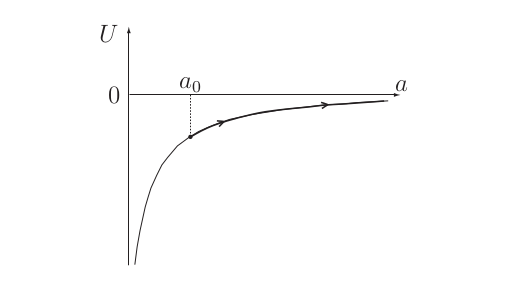
\includegraphics[width=15pc]{t12.png}
% \caption{}
%   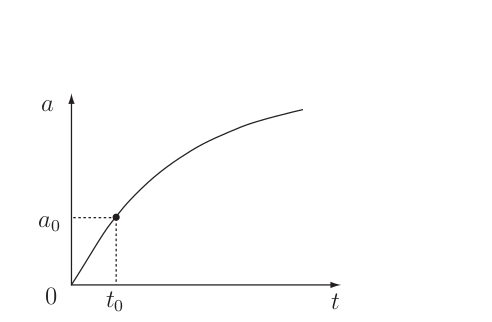
\includegraphics[width=15pc]{t13.png}
%   \caption{}
% \end{figure}
% 


\begin{figure}[h]
\begin{minipage}{14pc}
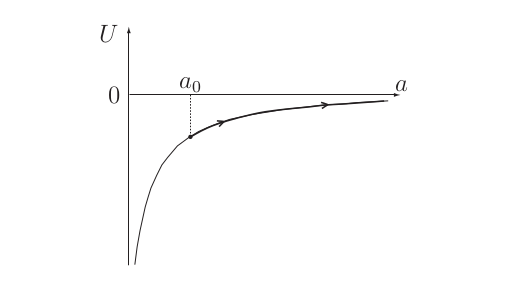
\includegraphics[width=15pc]{t12.png}
\caption{}
\end{minipage}\hspace{3pc}%
\begin{minipage}{14pc}
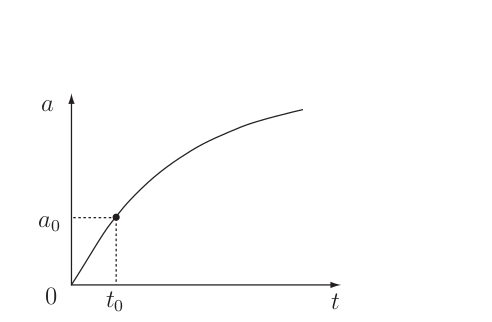
\includegraphics[width=15pc]{t13.png}
\caption{}
\end{minipage}\hspace{3pc}%
\end{figure}



En conclusion, le futur de l'Univers d\'epend de son contenu. S'il y a beaucoup de mati\`ere, l'Univers va s'effondrer ("Big Crunch"), autrement il y aura une expansion   infinie. Les observations astronomiques actuelles favorisent une expansion infinie de l'Univers.
\end{enumerate}
 
 
  
\chapter{L'acc\'el\'eration de l'Univers et mod\`eles de gravit\'e}\label{chapitre4}
\minitoc


Ce chapitre est consacr\'e \`a l'acc\'el\'eration de l'Univers, et aux mod\`eles physiques qui
permettent de l'expliquer. Apr\`es avoir rappel\'e les \'el\'ements de la cosmologie dont nous 
aurons besoin par la suite, nous d\'etaillerons les principales observations qui d\'emontrent que
l'Univers est actuellement dans une phase d'expansion acc\'el\'er\'ee. Nous pr\'esenterons ensuite
un panorama des mod\`eles ayant pour objectif d'expliquer cette acc\'el\'eration. Nous verrons
que certains mod\`eles se basent sur la Relativit\'e G\'en\'erale et la pr\'esence d'\'energie noire,
tandis que d'autres proposent un changement plus radical de paradigme, en modifiant les
lois de la gravit\'e.
\section{Le mod\`ele cosmologique standard}

\subsection{M\'etrique de FLRW }
Le mod\`ele cosmologique standard se base sur le fait que l'Univers autour de nous
appara\^it comme \'etant isotrope \`a grandes \'echelles, tant au niveau de la r\'epartition des
galaxies que du fond diffus cosmologique. Si l'on suppose de plus que notre Terre n'occupe
pas de place privil\'egi\'ee dans l'Univers, on en arrive au principe cosmologique qui fait
l'hypoth\`ese que l'Univers est spatialement homog\`ene et isotrope \`a grandes \'echelles.
La mod\'elisation math\'ematique de cette hypoth\`ese nous am\`ene \`a d\'ecrire l'espace-temps
par une m\'etrique de Friedmann-Lema\^itre-Robertson-Walker (FLRW) $ g_{\mu \nu} $ dont la forme
g\'en\'erale \cite{215, 277, 282} s'\'ecrit

\begin{eqnarray}
 ds^2 \equiv g_{ \mu \nu } dx^\mu dy^\nu = - dt^2  + a^2(t)[ d\chi^2 + f^2_K(\chi)(d\theta^2 + sin^2 \theta d\phi^2 ) ] \label{gene1} 
\end{eqnarray}

o\`u $ \chi $ est la coordonn\'ee radiale. La constante $K$ d\'ecrit la g\'eom\'etrie de la section spatiale
de l'espace-temps : l'espace est ferm\'e pour $ K > 0$, plat pour $K = 0$ et enfin ouvert pour
$K < 0$. La fonction $  f_K $ , qui est telle que la surface d'une sph\`ere de rayon $ \chi $ est donn\'ee par
    $ S(\chi ) = 4 \pi f_K^2(\chi) $, prend la forme 
   
   \begin{eqnarray}
   \qquad
   f_K(\chi) =  \begin{cases}
   K^{- \frac{1}{2}} sin( \sqrt{ K} \chi )  &\text{si }  K > 0 \\    \chi &\text{si } K = 0 \\ (-K)^{- \frac{1}{2}} sinh( \sqrt{ -K} \chi )
   &\text{si } K < 0
\end{cases}
    \end{eqnarray}

    La fonction $a(t)$ s'appelle le facteur d'\'echelle et caract\'erise l'\'evolution de l'Univers. On
normalise $ a(t) $ de telle sorte qu'aujourd'hui $ a \equiv a_0 = 1 $ (nous noterons avec un indice 0
la valeur des quantit\'es cosmologiques \'evalu\'ees aujourd'hui). Sa d\'ependance dans le temps
est d\'etermin\'ee en r\'esolvant les \'equations de la dynamique.

\subsection{Relativit\'e G\'en\'erale et \'equations de Friedmann}
Pour aller plus loin, il nous faut choisir une th\'eorie de la gravitation \`a partir de 
laquelle nous pourrons d\'eriver les \'equations de la dynamique pour le facteur d'\'echelle. La
cosmologie standard est bas\'ee sur la Relativit\'e G\'en\'erale $(RG)$ ; cependant, dans
cette th\`ese, nous travaillerons \'egalement avec d'autres th\'eories alternatives de la gravit\'e.
%(gravit\'e massive, mod\`ele $DGP$, th\'eories scalaire-tenseur, etc.) 
D'une th\'eorie \`a l'autre, les
\'equations de la dynamique varient, modifiant ainsi la cosmologie et l'interpr\'etation que
l'on peut faire des observations. C'est pr\'ecis\'ement l\`a tout l'int\'er\^et des th\'eories de gravit\'e
modifi\'ee, qui peuvent permettre de rendre compte des observations d'une fa\c{c}on diff\'erente
de la RG. Pour l'instant, nous voudrions
pr\'esenter le mod\`ele cosmologique standard, qui fait l'hypoth\`ese que la gravit\'e est d\'ecrite
par la RG.

L'action de la RG s'\'ecrit

\begin{eqnarray}
 S = \frac{M_P^2}{2} \int d^4 x \sqrt{- g} R [g]  + S_{\text {mati\`ere} } [ g],
\end{eqnarray}
o\`u $ R[g]$ est le scalaire de Ricci et $ M_P $ est la masse de Planck qui est reli\'ee \`a la constante de
Newton $G$ \`a travers  la relation $ M_P^{ -2} = 8 \pi G $. La mati\`ere est suppos\'ee minimalement
coupl\'ee \`a la m\'etrique.

La variation de l'action de la RG par rapport \`a la m\'etrique m\`ene aux \'equations d'Einstein

\begin{eqnarray}
 G_\mu^\nu = 8 \pi G T_\mu^\nu, \label{gene4}
\end{eqnarray}
o\`u $ G_\mu^\nu \equiv R_\mu^\nu - \frac{1}{2} \delta_\mu^\nu R  $ est le tenseur d'Einstein et $T_\mu^\nu $ le tenseur \'energie-impulsion de la
mati\`ere
\begin{eqnarray}
 T_{\mu \nu }(x) \equiv - \frac{2}{\sqrt{- g} }\frac{ \delta }{ \delta g^{\mu \nu } (x) } S_{\text{mati\`ere} } [g].
\end{eqnarray}
Les identit\'es de Bianchi garantissent que la mati\`ere est conserv\'ee, c'est-\`a-dire que
\begin{eqnarray}
 \Delta_\nu T_\mu^\nu = 0.
\end{eqnarray}
L'hypoth\`ese d'homog\'en\'eit\'e et d'isotropie, ainsi que la forme ( \ref{gene1}) de la m\'etrique, 
impose au tenseur \'energie-impulsion de la mati\`ere d'\^etre celui d'un fluide parfait
    
\begin{eqnarray}
 T_\mu^\nu = diag( -\rho, P, P, P),
\end{eqnarray}
o\`u $ \rho $ est la densit\'e de la mati\`ere, et $P$ sa pression. Il est ensuite ais\'e d'obtenir, \`a partir
de l'expression ( \ref{gene1}) de la m\'etrique de $FLRW$ et des \'equations d'Einstein ( \ref{gene4}), les deux
\'equations ind\'ependantes dites de Friedmann
\begin{eqnarray}
 H^2 = \frac{8 \pi G \rho }{ 3 } - \frac{K}{ a^2 }, \label{gene5} \\ \frac{\ddot{a }}{a } = -\frac{4 \pi G }{3} ( \rho + 3 P), \label{gene5'}
\end{eqnarray}
o\`u $ H \equiv \dot{a} / a $ est le param\`etre de Hubble et un point repr\'esente une d\'eriv\'ee par rapport au
temps cosmique t. L'\'equation de conservation de la mati\`ere prend quant \`a elle la forme
\begin{eqnarray}
 \dot{ \rho} + 3H(\rho + P) = 0 \label{gene6}
\end{eqnarray}
Il est usuel de r\'e\'ecrire l'\'equation ( \ref{gene5}) sous la forme r\'eduite
\begin{eqnarray}
 \sum_{\substack{i}} \Omega_i + \Omega_K = 1
\end{eqnarray}
o\`u l'indice $i$ correspond aux diff\'erents types de mati\`ere (radiation, mati\`ere noire, \'energie
noire, etc.) et o\`u l'on a d\'efini
\begin{eqnarray}
 \Omega_i \equiv \frac{8 \pi G \rho_i}{3 H^2},  \\ \Omega_K \equiv - \frac{K}{a^2 H^2}
\end{eqnarray}

Les observations \cite{177} montrent que la courbure spatiale est tr\`es proche de z\'ero, 
conform\'ement aux pr\'edictions g\'en\'eriques des mod\`eles d'inflation (cf. par exemple \cite{215}
; nous consid\'ererons donc par la suite dans ce m\'emoire que l'Univers est plat et fixerons
par cons\'equent $ K = 0 $.
 
 \subsection{Equation d'\'etat de la mati\`ere et \'evolution de l'Univers
%\'equation d'\'etat
}

La description la plus simple de la mati\`ere consiste \`a supposer que la densit\'e et la
pression de la mati\`ere suivent une \'equation d'\'etat de la forme
\begin{eqnarray}
  P = \omega \rho   \label{gene14}
\end{eqnarray}
o\`u $ \omega $ est suppos\'e constant. La mati\`ere sans pression (mati\`ere noire froide ) est d\'ecrite
par $ \omega = 0 $ tandis que le rayonnement a une \'equation d'\'etat  $ \omega = 1/3 $. Dans le cas d'une
constante cosmologique, $ \omega = -1 $.

Une fois muni de l'\'equation d'\'etat ( \ref{gene14}), il est ais\'e d'int\'egrer les \'equations de 
Friedmann ( \ref{gene5}) et (\ref{gene5'}) et l'\'equation de conservation de la mati\`ere ( \ref{gene6}) ; pour $ \omega \neq  -1 $, on
obtient
\begin{eqnarray}
 H = \frac{2}{ 3(1 +  \omega )(t - \bar{t}) } \label{gene15}  \\ a(t) \propto  (t- \bar{t})^{ \frac{2}{ 3(1+ \omega)}} \label{gene19} \\
 \rho \propto a^{ -3( 1 + \omega)} \label{gene20}
\end{eqnarray}
o\`u $\bar{t}$ correspond au d\'ebut de l'\`ere consid\'er\'ee. Pour $ \omega  = -1$, l'Univers est en acc\'el\'eration
et correspond \`a un espace de de Sitter tel que
\begin{eqnarray}
 H = cste  \\ a(t) \propto e^{H t}  \\ \rho = cste.
\end{eqnarray}
En utilisant la d\'ependance de $ \rho $ en a, on peut exprimer $H$ en fonction du contenu en
mati\`ere de l'Univers, gr\^ace \`a l'expression
\begin{eqnarray}
 H^2 = H_0^2 \Biggl( \sum_{\substack{i}} \Omega_{i,0} a^{-3(1 + \omega_i)} \Biggl) = 
 H_0^2 \Biggl( \sum_{\substack{i}} \Omega_{i,0} (1+z)^{3(1 + \omega_i)} \Biggl), \label{gene21}
\end{eqnarray}
o\`u l'on a introduit le redshift $  z \equiv  a^{-1} - 1 $. En int\'egrant cette \'equation, on peut obtenir
l'\'evolution du facteur d'\'echelle $ a(t)$.

{\bf Des origines \`a nos jours}

Selon le mod\`ele cosmologique standard, l'histoire de l'Univers peut se d\'ecomposer en
une succession d'\'etapes (encore appel\'ees \`eres), que nous r\'esumons ci-dessous.

La nature de la premi\`ere phase de l'\'evolution de l'Univers, entre l'origine de l'Univers et
le Big Bang chaud, n'est pas encore bien \'etablie, car il est tr\`es difficile de tester les mod\`eles
cosmologiques \`a des \'epoques aussi recul\'ees. Le mod\`ele de l'inflation est cependant devenu
le paradigme standard. Il s'agit d'une phase d'expansion acc\'el\'er\'ee durant laquelle $  \omega \simeq -1 $.
Cette phase d'acc\'el\'eration permet de donner une explication naturelle au probl\`eme de la
platitude (le fait que l'espace apparaisse plat \`a l'heure actuelle, ce qui ne peut \^etre le cas que
si l'espace \'etait extr\^emement plat aux \'echelles de Planck) et au probl\`eme de l'horizon (le fait
que des zones du ciel causalement ind\'ependantes aient une temp\'erature comparable \`a  $ 10^{-5}$
pr\`es). On consid\`ere g\'en\'eralement que cette phase d'inflation est domin\'ee par un champ
scalaire (ou plusieurs champs scalaires pour les mod\`eles multi-champs) appel\'e inflaton, en
r\'egime de roulement lent (cf. par exemple \cite{215}). Les perturbations quantiques
de ce champ sont la source des perturbations de la mati\`ere que l'on peut observer dans les
grandes structures et le fond diffus cosmologique (CMB). \`A l'issue de l'inflation, l'inflaton
se d\'esint\`egre en un grand nombre de particules : c'est la phase de r\'echauffement.

La suite de l'histoire de l'Univers est bien comprise, et est d\'ecrite par le mod\`ele du Big
Bang chaud :

- la premi\`ere phase qui suit le Big Bang chaud est l'\`ere de radiation, domin\'ee par
le rayonnement (photons et neutrinos). Cette phase dure jusqu'\`a l'\'egalit\'e mati\`ere-rayonnement, 
c'est-\`a-dire jusqu'au moment o\`u la densit\'e de la mati\`ere commence \`a
dominer la densit\'e d'\'energie du rayonnement (le redshift correspondant est $z_{eq} + 1  \equiv a_{eq}^{-1} \simeq 3600 $

- L'\`ere de mati\`ere est domin\'ee par la mati\`ere noire (CDM). C'est le moment o\`u
se forment les grandes structures. C'est \'egalement durant l'\`ere de mati\`ere qu'a
lieu le d\'ecouplage entre les photons et les baryons (le redshift correspondant est
  $z_{dec} + 1  \equiv a_{dec}^{-1} \simeq 1100 $).
 Cela est d\^u \`a la recombinaison des protons et des 
 \'electrons libres qui s'assemblent pour former des atomes neutres. Apr\`es le d\'ecouplage,
les photons peuvent se propager librement dans l'Univers ; l'observation du CMB
correspond \`a l'observation de ces photons \'emis au moment du d\'ecouplage.

- Les observations r\'ecentes du CMB, des supernovae et des oscillations baryons-photons
(BAO) indiquent que l'Univers est entr\'e tardivement (aux alentours de \cite{75}   $ z_c \simeq 0,67 $
pour   $ \Omega_m = 0,3 $ ) dans une nouvelle phase d'expansion acc\'el\'er\'ee, telle que  $  \omega \simeq -1  $.

Cette derni\`ere observation, \`a savoir que l'Univers est actuellement dans une phase 
d'expansion acc\'el\'er\'ee, constitue la motivation premi\`ere des th\'eories de gravit\'e modifi\'ee que
nous \'etudierons dans ce m\'emoire de th\`ese.
% Nous chercherons notamment \`a r\'epondre aux
% question suivantes : quelle peut \^etre la source de cette acc\'el\'eration, et comment contraindre
% exp\'erimentalement les propri\'et\'es physiques de cette source ?
% Avant de nous tourner vers ces questions , 
Nous voudrions
consacrer la prochaine section \`a la mod\'elisation de la source d'\'energie responsable de
cette acc\'el\'eration et que l'on appelle commun\'ement \'energie noire, ainsi qu'aux preuves
exp\'erimentales de son existence.

\section{Mod\'elisation et preuves exp\'erimentales de l'existence de
l'\'energie noire}
\subsection{Mod\'elisation de l'\'energie noire}
La source de l'acc\'el\'eration de l'Univers observ\'ee aujourd'hui est mal connue ; c'est
pourquoi on lui donne souvent le nom d'\'energie noire, traduisant ainsi le caract\`ere effectif
de cette description. On peut mod\'eliser cette \'energie noire par le tenseur \'energie impulsion
d'un fluide parfait
\begin{eqnarray}
 T_\mu^{de\, \nu} = diag( -\rho_{de}, P_{de}, P_{de}, P_{de}), \label{gene22}
\end{eqnarray}

la forme ci-dessus \'etant impos\'ee par l'hypoth\`ese d'homog\'en\'eit\'e et d'isotropie de l'Univers
qui est \`a la base de notre \'etude. On peut d\'efinir l'\'equation d'\'etat
\begin{eqnarray}
 \omega_{de} \equiv P_{de}/\rho_{de}
\end{eqnarray}
qui doit \^etre telle que
\begin{eqnarray}
 \omega_{de}<-1/3
\end{eqnarray}
pour que la phase domin\'ee par l'\'energie noire soit une phase d'acc\'el\'eration. La densit\'e
r\'eduite d'\'energie noire est mesur\'ee par
\begin{eqnarray}
 \Omega_{de} \equiv \frac{8 \pi G \rho_{ de}}{3 H^2} \label{gene25}
\end{eqnarray}
Les fonctions $ \Omega_{de}(a) $  et $ \omega_{de}(a) $ sont reli\'ees l'une \`a l'autre au travers de l'\'equation (\ref{gene20}),
qui dans le cas de l'\'energie noire, prend la forme
\begin{eqnarray}
 \Omega_{de} = \Omega_{de,0}a^{-3(\omega_{de} +1)}
\end{eqnarray}
Nous verrons \`a la Section\ref{emilo}  diff\'erents mod\`eles visant \`a d\'ecrire la nature de cette
\'energie noire. Il pourra s'agir d'une source de mati\`ere (champ scalaire par exemple), 
responsable de l'acc\'el\'eration. Il est \'egalement possible que les lois de la gravit\'e ne soient pas
celles de la RG, auquel cas l'interpr\'etation de l'\'energie noire comme une \'energie n'est pas
\`a prendre au sens litt\'eral ; cependant, comme les cons\'equences de ces modifications de la
gravit\'e ne peuvent pas \^etre distingu\'ees des effets qu'auraient une source d'\'energie de la
forme ( \ref{gene22}), nous d\'ecrirons la source de l'acc\'el\'eration de l'Univers, telle qu'elle soit,
par le tenseur \'energie impulsion (\ref{gene22}), et appellerons le ph\'enom\`ene responsable {\bf  \'energie 
noire}.

D'un point de vue pratique, on peut d\'ecrire en premi\`ere approximation l'impact de
cette \'energie noire par une constante cosmologique $ \Lambda$ telle que   $ \rho_\Lambda = - P_\Lambda = \Lambda / ( 8 \pi G)$ . Les
observations permettent d'\'evaluer
\begin{eqnarray}
 \Omega_\Lambda = \frac{\Lambda}{ 3 H_0^2} \simeq 0,7.
\end{eqnarray}
Nous voudrions \`a pr\'esent d\'ecrire plus en d\'etail les m\'ethodes astrophysiques et 
cosmologiques qui prouvent l'existence de l'\'energie noire. La plupart des valeurs num\'eriques qui
seront donn\'ees correspondent au cas d'une constante cosmologique (mod\`ele dit $ \Lambda CDM $),
qui est la param\'etrisation la plus simple de l'\'energie noire. Il faut bien s\^ur garder \`a l'esprit
qu'une param\'etrisation plus fine peut se r\'ev\'eler plus r\'ealiste. Le r\'esultat principal reste
cependant le m\^eme, quelque soit le cadre dans lequel on l'interpr\`ete : une composante
d'\'energie noire est n\'ecessaire pour expliquer les observations que sont les Supernovae de
type Ia, l'\^age apparent de l'Univers, la position des pics acoustiques du $CMB$ et la signature
des oscillations baryons-photons dans les grandes structures.


% 
%  \section{Mod\'elisation et preuves exp\'erimentales de l'existence de
% l'\'energie noire}
% \subsection{Mod\'elisation de l'\'energie noire}
% La source de l'acc\'el\'eration de l'Univers observ\'ee aujourd'hui est mal connue ; c'est
% pourquoi on lui donne souvent le nom d'\'energie noire, traduisant ainsi le caract\`ere effectif
% de cette description. On peut mod\'eliser cette \'energie noire par le tenseur \'energie impulsion
% d'un fluide parfait
% \begin{eqnarray}
%  T_\mu^{de\, \nu} = diag( -\rho_{de}, P_{de}, P_{de}, P_{de}), \label{gene22}
% \end{eqnarray}
% 
% la forme ci-dessus \'etant impos\'ee par l'hypoth\`ese d'homog\'en\'eit\'e et d'isotropie de l'Univers
% qui est \`a la base de notre \'etude. On peut d\'efinir l'\'equation d'\'etat
% \begin{eqnarray}
%  \omega_{de} \equiv P_{de}/\rho_{de}
% \end{eqnarray}
% qui doit \^etre telle que
% \begin{eqnarray}
%  \omega_{de}<-1/3
% \end{eqnarray}
% pour que la phase domin\'ee par l'\'energie noire soit une phase d'acc\'el\'eration. La densit\'e
% r\'eduite d'\'energie noire est mesur\'ee par
% \begin{eqnarray}
%  \Omega_{de} \equiv \frac{8 \pi G \rho_{ de}}{3 H^2} \label{gene25}
% \end{eqnarray}
% Les fonctions $ \Omega_{de}(a) $  et $ \omega_{de}(a) $ sont reli\'ees l'une \`a l'autre au travers de l'\'equation (\ref{gene20}),
% qui dans le cas de l'\'energie noire, prend la forme
% \begin{eqnarray}
%  \Omega_{de} = \Omega_{de,0}a^{-3(\omega_{de} +1)}
% \end{eqnarray}
% Nous verrons \`a la Section\ref{emilo}  diff\'erents mod\`eles visant \`a d\'ecrire la nature de cette
% \'energie noire. Il pourra s'agir d'une source de mati\`ere (champ scalaire par exemple), 
% responsable de l'acc\'el\'eration. Il est \'egalement possible que les lois de la gravit\'e ne soient pas
% celles de la RG, auquel cas l'interpr\'etation de l'\'energie noire comme une \'energie n'est pas
% \`a prendre au sens litt\'eral ; cependant, comme les cons\'equences de ces modifications de la
% gravit\'e ne peuvent pas \^etre distingu\'ees des effets qu'auraient une source d'\'energie de la
% forme ( \ref{gene22}), nous d\'ecrirons la source de l'acc\'el\'eration de l'Univers, telle qu'elle soit,
% par le tenseur \'energie impulsion (\ref{gene22}), et appellerons le ph\'enom\`ene responsable {\bf  \'energie 
% noire}.
% 
% D'un point de vue pratique, on peut d\'ecrire en premi\`ere approximation l'impact de
% cette \'energie noire par une constante cosmologique $ \Lambda$ telle que   $ \rho_\Lambda = - P_\Lambda = \Lambda / ( 8 \pi G)$ . Les
% observations permettent d'\'evaluer
% \begin{eqnarray}
%  \Omega_\Lambda = \frac{\Lambda}{ 3 H_0^2} \simeq 0,7.
% \end{eqnarray}
% Nous voudrions \`a pr\'esent d\'ecrire plus en d\'etail les m\'ethodes astrophysiques et 
% cosmologiques qui prouvent l'existence de l'\'energie noire. La plupart des valeurs num\'eriques qui
% seront donn\'ees correspondent au cas d'une constante cosmologique (mod\`ele dit $ \Lambda CDM $),
% qui est la param\'etrisation la plus simple de l'\'energie noire. Il faut bien s\^ur garder \`a l'esprit
% qu'une param\'etrisation plus fine peut se r\'ev\'eler plus r\'ealiste. Le r\'esultat principal reste
% cependant le m\^eme, quelque soit le cadre dans lequel on l'interpr\`ete : une composante
% d'\'energie noire est n\'ecessaire pour expliquer les observations que sont les Supernovae de
% type Ia, l'\^age apparent de l'Univers, la position des pics acoustiques du $CMB$ et la signature
% des oscillations baryons-photons dans les grandes structures.

\subsection{Supernovae de type Ia}
La preuve la plus directe que notre Univers est actuellement en expansion acc\'el\'er\'ee
est donn\'ee par la mesure de la distance des luminosit\'es des supernovae de type $Ia$ (SN Ia). La
distance luminosit\'e d'un objet astrophysique de luminosit\'e intrins\`eque $L_{\text{source}}$ et situ\'e \`a
un redshift $z$ est d\'efinie de telle sorte que le flux observ\'e $ \Phi_{obs}$ est donn\'e par
\begin{eqnarray}
 \Phi_{obs} = \frac{L_{source}}{ 4 \pi D_L^2} \label{gene28}
\end{eqnarray}
On peut montrer \cite{267} que dans un Univers (plat) en expansion, $D_L$ est donn\'ee par
\begin{eqnarray}
 D_L = \frac{1}{H_0} (1 + z) \int_0^z \frac{dz'}{\sqrt{ \sum_{i}  \Omega_{i,0}(1+z')^{3(1 + \omega_i) }}} \label{gene29}
\end{eqnarray}
o\`u les $ \Omega_{i,0} $ sont les densit\'es r\'eduites de chaque composante de mati\`ere ($y$ compris l'\'energie
noire).

Pour des objets proches ($ z  \ll 1 $), on voit que la formule ( \ref{gene29}) se r\'esume \`a $ z \sim H_0 D_L $.
D'autre part, on peut montrer que le redshift est reli\'e \`a la vitesse de r\'ecession des galaxies
au travers de $ z \equiv  a^{-1} - 1 \sim v $ ; on obtient donc que pour des petits redshifts $ v \sim H_0 D_L $.
On retrouve l\`a la loi de Hubble qui permet de mesurer $H_0$ \`a partir de l'observation de la
vitesse de r\'ecession des galaxies. Pour des objets plus lointains, on voit que l'expression
de la distance luminosit\'e d\'epend du contenu en \'energie de l'Univers, au travers de la
racine carr\'ee de l'\'equation ( \ref{gene29}). La mesure de la fonction $ D_L(z) $ permet donc de mesurer
le r\^ole jou\'e par les diff\'erentes composantes de mati\`ere $ \Omega_{i,0} $ . Cependant, pour mesurer la
distance luminosit\'e d'objets au travers de la d\'efinition ( \ref{gene28}), encore faut-il conna\^itre leurs
luminosit\'es intrins\`eques.

C'est pr\'ecis\'ement le cas des  $ SN Ia$, qui peuvent \^etre observ\'ees lorsqu'une naine blanche
d'un syst\`eme binaire a accr\'et\'e tellement de mati\`ere en provenance de son compagnon que
sa masse a atteint la masse de Chandrasekhar ; elle s'effondre alors et explose en supernova.
La courbe de lumi\`ere des $ SN Ia $ est quasi-identique d'une supernova \`a l'autre : ce sont des
chandelles standard. En 1998, deux \'equipes ont publi\'e ind\'ependamment le diagramme de
Hubble $ D_L(z) $ de deux catalogues de $ SN Ia $ : le groupe Supernova Cosmology Project (SCP)
\cite{213} a ainsi mesur\'e la distance luminosit\'e de 42 $SN Ia$ de redshift $ z \in [0.18; 0.8]$, tandis
que les membres de la High-Z Supernova Search Team (HSST) \cite{224} ont identifi\'e 24 $SN Ia$
proches et 14 $SN Ia$ dans l'intervalle $ z \in [0.16; 0.62]$ . Ces observations (ainsi que d'autres
mesures qui ont eu lieu depuis lors, parmi lesquelles on peut citer \cite{26, 171, 195, 225} ont
permis d'\'ecarter la possibilit\'e que l'Univers soit plat et constitu\'e uniquement de mati\`ere
 $( \Omega_m = 1)$. Il est donc n\'ecessaire d'inclure une composante d'\'energie noire, comme on peut
le voir sur la Fig.\ref{figgene1} .

% \begin{figure}[h]
% 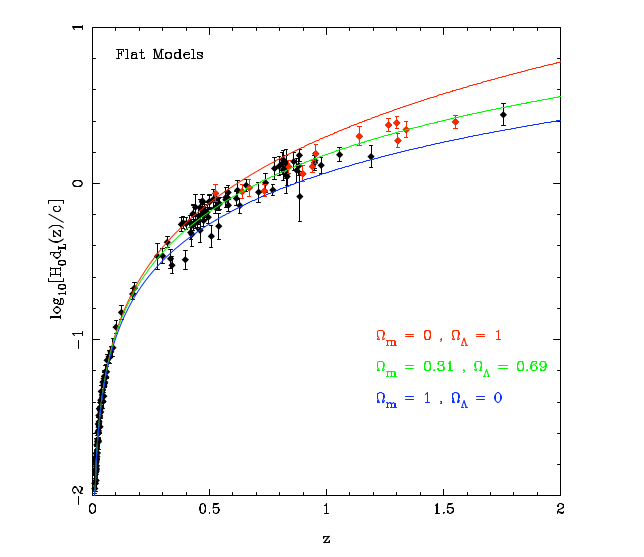
\includegraphics[width=30pc]{figgene1.png}
% \caption{\label{figgene1} Diagramme de Hubble (distance luminosit\'e $ \log [H_0 D_L(z) ] $ en fonction du 
% red-shift $z$) pour un Univers plat pour un certain nombres de SN Ia observ\'ees. Les points
% noirs proviennent du catalogue “Gold” de Riess et al. $[225]$, tandis que les points rouges
% proviennent de mesures effectu\'ees par le Hubble Space Telescope $(HST)$. On voit tr\`es 
% clairement que le cas $ \Omega_m = 0.31$, $ \Omega_\Lambda = 0.69$ correspond mieux aux observations que le cas d'un
% univers sans constante cosmologique $ \Omega_m = 1$, $ \Omega_\Lambda = 0$ . La figure provient de la r\'ef\'erence
% $[71]$. 
%  }
% \end{figure}

\begin{figure}[h]
%\begin{minipage}{14pc}
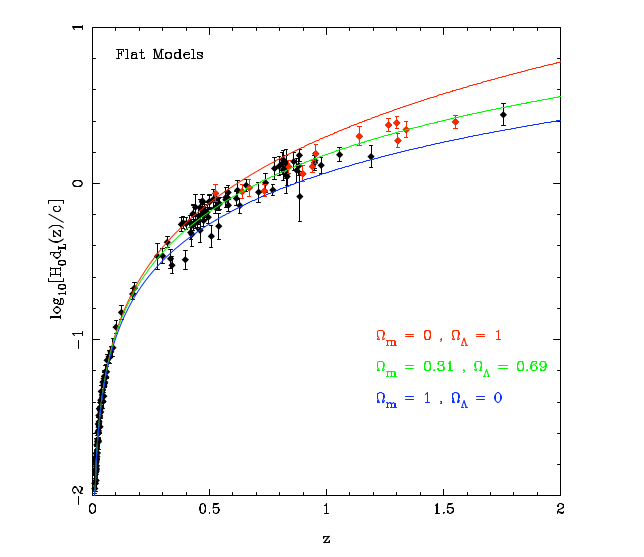
\includegraphics[width=30pc]{figgene1.png}
\caption{\label{figgene1} Diagramme de Hubble (distance luminosit\'e $ \log [H_0 D_L(z) ] $ en fonction du 
red-shift $z$) pour un Univers plat pour un certain nombres de SN Ia observ\'ees. Les points
noirs proviennent du catalogue ''Gold'' de Riess et al. \cite{225}, tandis que les points rouges
proviennent de mesures effectu\'ees par le Hubble Space Telescope $(HST)$. On voit tr\`es 
clairement que le cas $ \Omega_m = 0.31$, $ \Omega_\Lambda = 0.69$ correspond mieux aux observations que le cas d'un
univers sans constante cosmologique $ \Omega_m = 1$, $ \Omega_\Lambda = 0$ . La figure provient de la r\'ef\'erence
\cite{71}.}
%\end{minipage}\hspace{3pc}%
% \begin{minipage}{14pc}
% 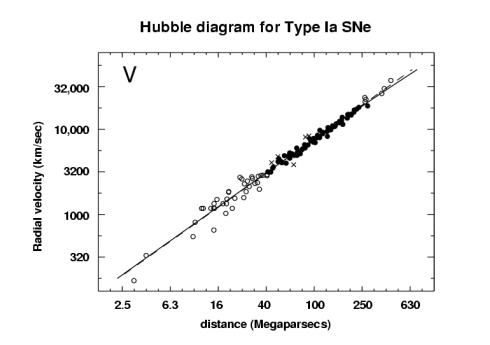
\includegraphics[width=15pc]{t4.png}
%  \caption{Diagramme de Hubble (pour
% les supernovae) de $2005$ \cite{2}}
%  \end{minipage}\hspace{3pc}%
\end{figure}



% 
% Utilis\'ees toutes seules, les donn\'ees des SN Ia ne peuvent pas contraindre tr\`es 
% pr\'ecis\'ement $ \Omega_\Lambda $ ou $ \Omega_m $, mais seulement une combinaison des deux param\`etres; cela est d\^u \`a la
% forme elliptique des contraintes (cf. Fig. \ref{figgene2}). Nous verrons qu'il est possible d'am\'eliorer
% consid\'erablement la pr\'ecision des mesures en combinant ces mesures de distance luminosit\'e
% avec d'autres donn\'ees (CMB, BAO,...).
% 
  \begin{figure}[h]
 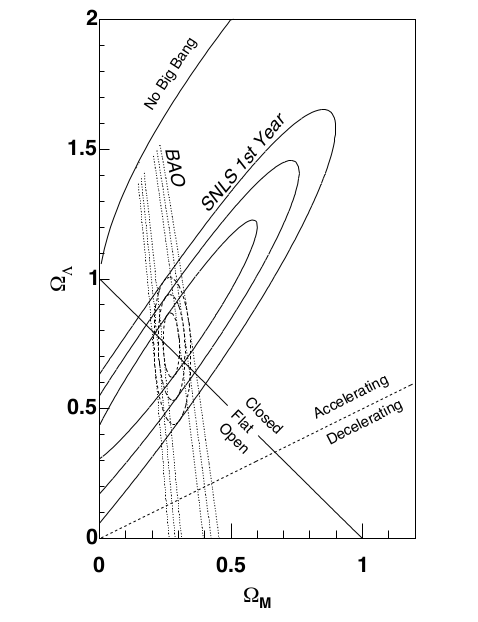
\includegraphics[width=20pc]{figgene2.png}
 \caption{\label{figgene2} Contours des niveaux de confiance \`a $ 68.3 \% $, $ 95.5 \% $ et $ 99.7 \% $ pour les param\`etres
 $ (\Omega_m, \Omega_\Lambda )$, issues du diagramme de Hubble obtenu par le Supernova Legacy Survey (SNLS)
 (lignes pleines) et des BAO mesur\'ees par le Sloan Digital Sky Survey (SDSS) (lignes 
 pointill\'ees). Les contraintes conjointes sont repr\'esent\'ees par les lignes en pointill\'es larges. Le
 cas $ (\Omega_m, \Omega_\Lambda ) = (1, 0)$ est tr\`es clairement exclu. Les valeurs des param\`etres $ (\Omega_m, \Omega_\Lambda )$ 
 favoris\'ees par les donn\'ees des SN Ia sont dans une ellipse orient\'ee selon une droite d'\'equation
   $  \Omega_\Lambda \backsimeq  \Omega_m + 0.4 $ . La figure ci-dessus est issue de \cite{26}.
   }
 \end{figure}



 
 \subsection{ \^Age de l'Univers }
 Au moment du Big Bang chaud (qui correspond \`a la fin de l'inflation dans les mod\`eles
inflationnaires) que l'on prendra par convention \`a $ t = 0$, on doit avoir  $ a(t = 0) \geqslant 0 $. On en
d\'eduit donc que le temps $t_0$ \'ecoul\'e depuis le Big Bang est born\'e par
\begin{eqnarray}
 t_0 = \int_{\tau_0}^{\tau_1} dt = \int_{a(t=0)}^{a_0 = 1} \frac{dt}{ da} da \leqslant \int_{0}^{ 1} \frac{dt}{ da} da =
 \int_{0}^{ 1} \frac{da}{ aH}   \label{gene30}
\end{eqnarray}
Si on utilise l'\'equation ( \ref{gene21}) et l'on exprime l'int\'egrale en fonction du redshift $z$ on obtient
\begin{eqnarray}
 t_0 \leqslant \int_{0}^{\infty } \frac{dz}{(1 + z)H(z) } = \frac{1}{H_0}
 \int_0^{\infty} \frac{dz}{ (1 + z) \sqrt{ \sum_{i}  \Omega_{i,0}(1+z)^{3(1 + \omega_i) }}}, \label{gene31}
\end{eqnarray}
o\`u l'indice $i$ correspond \`a la radiation, la mati\`ere noire et \`a l'\'energie noire, que l'on 
mod\'elisera par une constante cosmologique. On peut n\'egliger dans l'int\'egrale ci-dessous la
contribution de la radiation, car l'\`ere de radiation est tr\`es courte compar\'ee aux \`eres 
suivantes. On voit donc que l'\^age de l'Univers d\'epend des param\`etres $(\Omega_m, \Omega_{de} )$. Dans le cas
d'un univers domin\'e par la mati\`ere tel que $\Omega_m = 1$, on peut calculer explicitement 
l'int\'egrale de l'\'equation (\ref{gene31}) et obtenir la borne $ t_0 \leqslant 2 /(3H_0)$. En utilisant la valeur de la
constante de Hubble trouv\'ee par l'\'equipe du Hubble Key Project \cite{126} $ H_0 = 72 \pm 8 km.s^{-1} Mpc^{-1} $,
% on trouve que $t_0 = 8 − 10 $ milliards d'ann\'ees. Cette valeur de l'\^age de l'Univers
%doit \^etre compar\'ee \`a l'\^age des plus vieux objets stellaires connus, qui est d'environ $ 11 − 13$
milliards d'ann\'ees \cite{143, 163, 223}. {\bf  \`A l'\'evidence, le cas d'un Univers domin\'e uniquement par
 la mati\`ere est donc en contradiction avec l'\^age de ces objets.} Cette difficult\'e peut \^etre
r\'esolue en supposant la pr\'esence d'\'energie noire. Ainsi, si l'on fait l'hypoth\`ese que 
l'\'energie noire prend la forme d'une constante cosmologique telle que $(\Omega_m, \Omega_{\Lambda} ) = (0.3, 0.7)$, on
trouve que  $ t_0 \backsimeq 13.1$ milliards d'ann\'ees, {\bf ce qui n'est plus contradictoire avec l'\^age des plus
vieux objets connus dans l'Univers. Ceci est donc un \'el\'ement suppl\'ementaire en faveur de
la pr\'esence d'\'energie noire dans l'Univers.}
 
 \subsection{Fond diffus cosmologique}
 
 Une preuve ind\'ependante de l'existence d'\'energie noire dans l'Univers peut \^etre obtenue
\`a partir de la position des pics acoustiques du fond diffus cosmologique (CMB). En effet,
on peut montrer \cite{215} que la position dans l'espace des multip\^oles du n-i\`eme pic est donn\'ee
dans le cas de perturbations primordiales adiabatiques par
\begin{eqnarray}
  l_{(n)} = n \pi \frac{D_A(z_{LSS})}{r_s (z_{LSS}) }, \;\;\;\; n = 1, \; 2, \; ... \label{gene32}
\end{eqnarray}
o\`u nous avons introduit l'horizon sonique co-mobile
\begin{eqnarray}
 r_s(z) \equiv \int_z^{\infty } \frac{C_s(z')}{H(z') }dz', \label{gene33}
\end{eqnarray}
et le diam\`etre angulaire co-mobile
\begin{eqnarray}
 D_A = \frac{1}{H_0} \frac{1}{1+z} \int_0^z \frac{dz'}{\sqrt{ \sum_{i}  \Omega_{i,0}(1+z')^{3(1 + \omega_i) }}} \label{gene34}
\end{eqnarray}
Dans les expressions ci-dessus, $z_{LSS} \simeq  1100 $ est le redshift de la surface de derni\`ere 
diffusion  et $c_s$ est la vitesse du son du fluide baryon-photon dont les oscillations avant la
recombinaison sont \`a l'origine des pics du CMB. Le rayon sonique $ r_s(z{LSS})$ d\'epend de
la quantit\'e de baryons dans l'Univers $ \Omega_b $ et est ind\'ependant de l'\'energie noire car cette
derni\`ere ne joue aucun r\^ole \`a des temps aussi anciens ; la hauteur des pics du CMB et en
particulier la diff\'erence entre la hauteur des pics pairs et impairs permet de mesurer $ \Omega_b $
(et donc $ r_s (z_{LSS} )$ ). On peut alors utiliser la mesure de la position des pics (\ref{gene32}) pour
contraindre l'\'energie noire, au travers de la d\'ependance du diam\`etre angulaire $ D_A(z_{LSS} )$
dans la g\'eom\'etrie de l'Univers.

Le spectre du CMB d\'epend \'egalement de l'\'energie noire au travers de l'effet 
SachsWolfe int\'egr\'e (ISW), qui permet de prendre en compte le fait que les photons du CMB ont
travers\'e sur leur chemin jusqu'\`a nous des puits de potentiel en \'evolution. L'\'evolution des
potentiels gravitationnels d\'ependant du contenu en mati\`ere de l'Univers, la mesure de cet
effet permet de contraindre la densit\'e d'\'energie noire, ainsi que son \'equation d'\'etat $ \omega_{de} $.

L'analyse des donn\'ees prises pendant $5$ ans \cite{177} par le satellite $WMAP$ a permis de
mesurer $ \Omega_\Lambda = 0.742 \pm 0.030 $ dans le cas d'une constante cosmologique. Dans le cas o\`u
l'\'equation d'\'etat de l'\'energie noire est \'egalement mesur\'ee, l'\'equipe de WMAP a obtenu
%l'intervalle de confiance \`a $95 \%$ :$ −1.37 < 1 + \omega_{de} < 0.32 $.
 
 \subsection{Oscillations Acoustiques des Baryons (BAO)}
 Les oscillations du fluide baryons-photons qui ont lieu avant la recombinaison ne sont
pas seulement observables dans le spectre du CMB, mais \'egalement dans les grandes 
structures. En effet, consid\'erons une sur-densit\'e \`a $ t = 0$; sous l'effet de la pression de la radiation,
cette sur-densit\'e s'\'etend \`a la vitesse du son du plasma, sous la forme d'une onde sph\'erique.

Au moment de la recombinaison, les densit\'es aux points situ\'es \`a une distance $ r_s (z_{LSS} )$
de la sur-densit\'e initiale sont donc corr\'el\'ees. De nos jours, cette corr\'elation est bien s\^ur
brouill\'ee, car les ondes sonores de diff\'erentes sur-densit\'es se sont superpos\'ees depuis ; il est
cependant possible de d\'etecter statistiquement la signature de l'\'echelle co-mobile $ r_s (z_{LSS} )$,
caract\'eristique des BAO, au travers de la mesure de la fonction de corr\'elation des galaxies.
En raison de l'expansion de l'Univers, cette \'echelle co-mobile (fixe depuis la recombinaison,
et qui vaut environ $ r_s (z_{LSS} ) \backsimeq 150 Mpc) $ est vue sous un angle
\begin{eqnarray}
 \theta_S = \frac{ r_s (z_{LSS} ) }{ D_A(z_{LSS} ) } \label{gene35}
\end{eqnarray}
o\`u le diam\`etre angulaire co-mobile $ D_A(z_{LSS} )$ a \'et\'e d\'efini \`a l'\'equation (\ref{gene34}). La premi\`ere
d\'etection de ce ph\'enom\`ene a eu lieu en 2005 par l'\'equipe du SDSS  \cite{115}; on voit sur
la figure \ref{figgene3} la signature tr\`es nette du rayon sonique dans la fonction de corr\'elation des
galaxies 8 du catalogue.

% \begin{figure}[h]
% 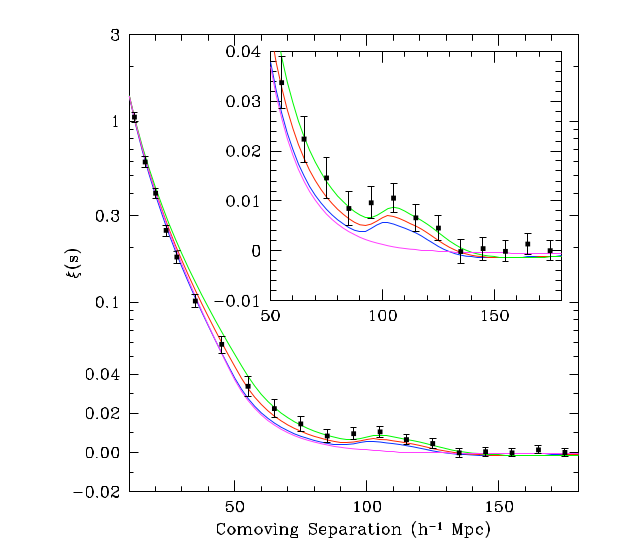
\includegraphics[width=35pc]{figgene3.png}
% \caption{\label{figgene3} Fonction de corr\'elation des galaxies du catalogue du SDSS. Les courbes verte
% (en haut), rouge et bleue (en bas, avec un pic) correspondent respectivement aux mod\`eles
%  $ \Omega_m h^2 =  0.12, 0.13, 0.14$, avec $ \Omega_b h^2 = 0.024 $. La courbe du bas (sans pic) correspond \`a un
% mod\`ele de mati\`ere noire sans baryon $ ( \Omega_m h^2 = 0.105) $. On voit tr\`es clairement la signature
% des BAO \`a $ r \backsimeq 105h^{-1}Mpc \backsimeq 150Mpc $. Figure issue de l'article \cite{115}.
%  }
% 
% \end{figure}

\begin{figure}[h]
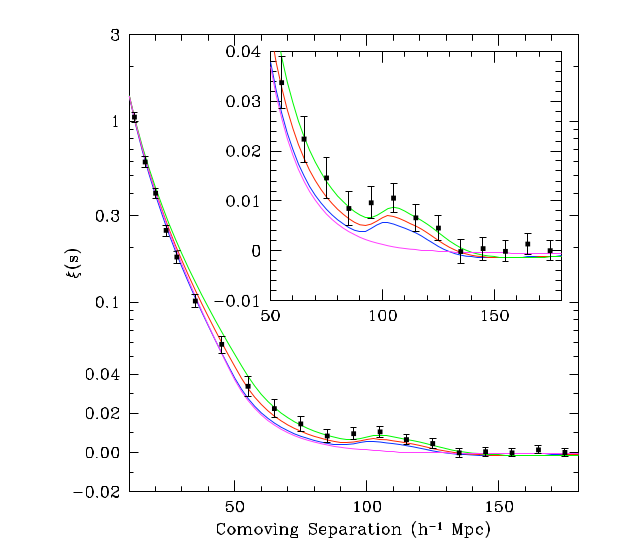
\includegraphics[width=25pc]{figgene3.png}
\caption{\label{figgene3} Fonction de corr\'elation des galaxies du catalogue du SDSS. Les courbes verte
(en haut), rouge et bleue (en bas, avec un pic) correspondent respectivement aux mod\`eles
 $ \Omega_m h^2 =  0.12, 0.13, 0.14$, avec $ \Omega_b h^2 = 0.024 $. La courbe du bas (sans pic) correspond \`a un
mod\`ele de mati\`ere noire sans baryon $ ( \Omega_m h^2 = 0.105) $. On voit tr\`es clairement la signature
des BAO \`a $ r \backsimeq 105h^{-1}Mpc \backsimeq 150Mpc $. Figure issue de l'article  \cite{115}.
 }
\end{figure}

Il est donc possible de tester le contenu en mati\`ere de l'Univers par l'\'etude des BAO,
et notamment la densit\'e d'\'energie noire $ \Omega_{de} $ et son \'equation d'\'etat $ \omega_{de} $ . En particulier,
l'observation des BAO donne des informations tr\`es pr\'ecieuses lorsqu'elles sont combin\'ees
avec d'autres observations, comme on peut le voir sur la figure \ref{figgene4}.
 
 \subsection{Mesures combin\'ees}
 Comme nous l'avons d\'ej\`a signal\'e ci-dessus, les m\'ethodes \'evoqu\'ees (SN Ia, CMB, BAO)
sont compl\'ementaires. En premier lieu, ces mesures provenant de processus physiques tr\`es 
diff\'erents et ind\'ependants, il est impressionnant qu'elles puissent mener \`a des mesures 
coh\'erentes : cela confirme d'une fa\c{c}on spectaculaire la robustesse du mod\`ele cosmologique
standard. De plus, les ellipses de contraintes associ\'ees \`a chacune de ces m\'ethodes ne sont
pas orient\'ees dans la m\^eme direction, comme on peut le voir sur la figure \ref{figgene4}. En combinant
ces mesures, on peut donc diminuer la d\'eg\'en\'erescence entre les diff\'erents param\`etres. En
proc\'edant de la sorte, Percival et al. \cite{212} ont mesur\'e, dans le cas d'un mod\`ele $ \Lambda CDM $,
$ (\Omega_m , \Omega_\Lambda ) = (0.288 \pm 0.018, 0.712  \pm 0.018)$.

L'existence d'une phase d'acc\'el\'eration r\'ecente de l'Univers est donc bien \'etablie. Nous
savons que l'on peut mod\'eliser la source de cette acc\'el\'eration par le tenseur \'energie-
impulsion d'un fluide parfait, que nous avons nomm\'e \'energie noire. Nous n'avons cependant
pas encore abord\'e la question de la nature physique de cette \'energie noire. C'est ce vers
quoi il nous faut \`a pr\'esent nous tourner.



	 \begin{figure}[h]
%\begin{minipage}{14pc}
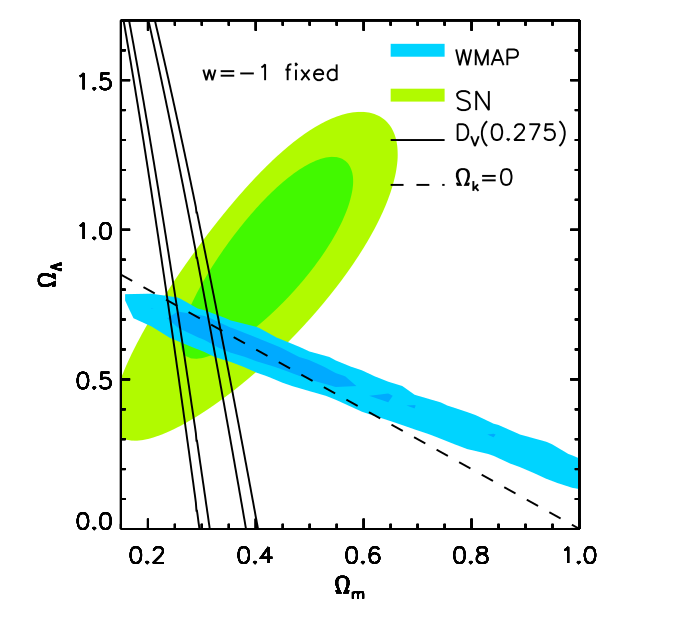
\includegraphics[width=25pc]{figgene4.png}
\caption{\label{figgene4} Combinaison des contraintes sur les param\`etres $( \Omega_m, \Omega_\Lambda )$ du mod\`ele $ \Lambda CDM$
issues de la mesure de la distance luminosit\'e des SN Ia (Union supernovae \cite{195}), du
CMB (WMAP5) et des BAO (SDSS - release 7). Les ellipses des contraintes associ\'ees des
trois types de mesures sont orient\'ees d'une fa\c{c}on tr\`es diff\'erente : l'association des trois
observations permet donc de mesurer les param\`etres $( \Omega_m, \Omega_\Lambda )$  beaucoup plus pr\'ecis\'ement
qu'avec chacune des m\'ethodes s\'epar\'ement. La figure provient de \cite{212}.
  }
%\end{minipage}\hspace{3pc}%
% \begin{minipage}{14pc}
% 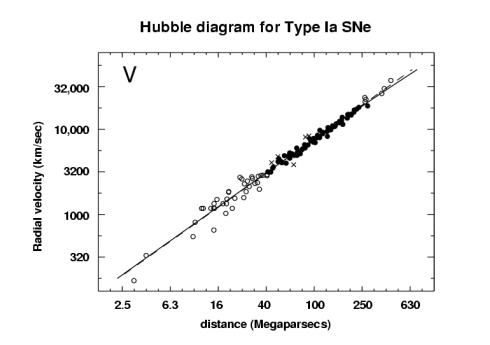
\includegraphics[width=15pc]{t4.png}
%  \caption{Diagramme de Hubble (pour
% les supernovae) de $2005$ \cite{2}}
%  \end{minipage}\hspace{3pc}%
\end{figure}


\newpage
 
 \section{\'Energie noire ou gravit\'e modifi\'ee ?} \label{emilo}
\subsection{Le probl\`eme de la constante cosmologique}
Nous avons d\'ej\`a vu que le mod\`ele le plus simple d'\'energie noire est simplement une
constante cosmologique $ \Lambda $ telle que $ \rho_\Lambda = -P_\Lambda =  \Lambda /(8 \pi G)$ et $ \Omega_\Lambda \backsimeq 0,7 $. Le probl\`eme
de ce mod\`ele est qu'il n'explicite pas vraiment l'origine physique de cette constante. La
source d'\'energie qui pourrait correspondre d'une fa\c{c}on a priori naturelle \`a une constante
cosmologique est l'\'energie du vide. Malheureusement, les ordres de grandeur des deux
ph\'enom\`enes n'ont rien en commun. La constante cosmologique est telle que la densit\'e correspondant vaut
\begin{eqnarray}
 \rho_\Lambda = 10^{-47}GeV   \label{gene36}
\end{eqnarray}
On peut d'autre part \'evaluer la densit\'e d'\'energie du vide, qui correspond \`a la somme sur
tous les modes, de l'\'energie de point z\'ero  $ \omega_k/2 $. Pour un champ scalaire, on obtient :
\begin{eqnarray}
 \rho_{vac} = \frac{1}{2} \int_0^{k_{max} } \frac{d^3k}{(2 \pi)^3} \sqrt{k^2 + m^2} \backsimeq  \frac{k^4_{max}}{ 16 \pi^2} \label{gene37}
\end{eqnarray}
o\`u $ k^4_{max} $ est le  cutoff
de la th\'eorie des champs que l'on consid\`ere et $m$ la masse du champ,
que l'on supposera  $ \ll k_{max} $ . Si l'on prend pour cutoff l'\'echelle de grande unification $ k_{max} =
E_{GUT} = 10^{16} GeV $, on obtient
\begin{eqnarray}
 \rho_{vac} \backsimeq 10^{62 } GeV^4 \ggg  \rho_\Lambda.  \label{gene38}
\end{eqnarray}

Le mod\`ele de la constante cosmologique est \'egalement insatisfaisant du point de vue de
l'explication de la valeur de sa densit\'e d'\'energie actuelle. Ce probl\`eme est connu sous le
nom de probl\`eme de la co\"{i}ncidence : pourquoi la densit\'e d'\'energie noire est-elle de l'ordre
de la densit\'e de la mati\`ere noire, pr\'ecis\'ement aujourd'hui, alors que les deux ph\'enom\`enes
ont a priori des origines tr\`es diff\'erentes. De plus, cette densit\'e, tr\`es faible, doit \^etre 
ajust\'ee tr\`es pr\'ecis\'ement : c'est ce qui est appel\'e le probl\`eme du fine tuning de la constante
cosmologique.

Ces difficult\'es d'ordre th\'eorique (d'un point de vue ph\'enom\'enologique, le mod\`ele $ \Lambda CDM $
est pour l'instant en tr\`es bon accord avec les observations) ont pouss\'e la communaut\'e des
physiciens des particules et des cosmologistes \`a se pencher plus en d\'etail sur les possibles
mod\`eles d'\'energie noire, au-del\`a du mod\`ele de la constante cosmologique. Nous allons 
pr\'esenter un panorama de ces mod\`eles (on pourra \'egalement consulter avec profit les articles
\cite{75, 211, 265}). Deux grandes cat\'egories de mod\`eles peuvent \^etre distingu\'ees : les mod\`eles
qui supposent que la RG d\'ecrit correctement les lois de la gravitation, et les mod\`eles de
gravit\'e modifi\'ee.

\subsection{Mod\`eles restant dans le cadre de la Relativit\'e G\'en\'erale}
La plupart des mod\`eles de cette cat\'egorie consistent \`a prendre litt\'eralement 
l'interpr\'etation du fluide parfait (\ref{gene22}) en tant qu'\'energie, et \`a postuler l'existence d'un ou de
plusieurs nouveaux champs responsables de l'acc\'el\'eration r\'ecente de l'Univers.

Les mod\`eles les plus simples de cette classe sont les mod\`eles de quintessence \cite{221, 284},
dans lesquelles l'\'energie noire est d\'ecrite par un champ scalaire en r\'egime de roulement
lent, d'une mani\`ere tout \`a fait semblable \`a l'inflaton. L'action de ce champ scalaire $ \varphi $ s'\'ecrit
\begin{eqnarray}
 S = \int d^4x\sqrt{-g} \Biggl( -\frac{1}{2}g^{ \mu \nu} \partial_{\mu \varphi} \partial_{ \nu \varphi} - V(\varphi) \Biggr), \label{gene39}
\end{eqnarray}
o\`u $V$ est le potentiel du champ. \`a partir de cette action, il est facile de calculer le tenseur
\'energie-impulsion du champ scalaire dans un univers homog\`ene et isotrope ; on peut alors
montrer que l'\'equation d'\'etat prend la forme
\begin{eqnarray}
 \omega_\varphi = \frac{\frac{1}{2}\dot{\varphi} - V(\varphi) }{\frac{1}{2}\dot{\varphi} + V(\varphi) }. \label{gene40}
\end{eqnarray}
On peut d\'efinir les param\`etres de roulements lents par
\begin{eqnarray}
 \epsilon \equiv  \frac{1}{16 \pi G} \Biggl( \frac{V_{, \varphi}}{V}  \Biggr)^2, \;\;\;\;
 \eta = \frac{1}{ 8 \pi G} \Biggl(  \frac{V_{,\varphi \varphi}}{ V}    \Biggr), \label{gene41}
\end{eqnarray}
o\`u $ V{,\varphi}$ est la d\'eriv\'ee du potentiel par rapport au champ scalaire. Dans la limite de roulement
lent
\begin{eqnarray}
 \epsilon \ll 1, \;\;\;\; \eta \ll 1, \label{bene42}
\end{eqnarray}
le champ scalaire peut jouer le r\^ole d'\'energie noire, avec une \'equation d'\'etat  $ \omega_\varphi \backsimeq -1 + 2 \epsilon / 3 $ .

Le potentiel $ V( \varphi)M^4 e^{- \lambda \varphi} $ est un exemple int\'eressant de potentiel, car on peut 
montrer que le r\'egime $ \omega \backsimeq -1 $ est un attracteur, c'est-\`a-dire que pour une grande plage de
conditions initiales, le champ $ \varphi $ entrera dans le r\'egime de roulement lent si l'on attend 
suffisamment longtemps. Ce m\'ecanisme d'attraction ne r\'esoud pas le probl\`eme du fine-tuning,
mais permet n\'eanmoins de donner une explication naturelle au fait que l'\'energie noire ait
une \'equation d'\'etat constante ou quasi-constante aujourd'hui.

De nombreux autres mod\`eles existent, parmi lesquels on peut citer les mod\`eles de 
tachyon \cite{241, 242, 243}, d'\'energie noire fantomale \cite{57, 59} ou encore de K-essence \cite{23, 24, 69}.

Une autre possibilit\'e pour expliquer l'acc\'el\'eration apparente de l'Univers sans modifier
les lois de la gravitation consiste \`a trouver un m\'ecanisme qui modifie la fa\c{c}on dont nous
percevons les photons qui se propagent depuis les SN Ia et autres ph\'enom\`enes observables.
C'est par exemple le cas lorsque les photons sont coupl\'es \`a un axion, et peuvent osciller
lors de la propagation dans le champ magn\'etique extra-galactique \cite{78, 99, 102}. Les objets
astrophysiques nous apparaissent alors plus lointains qu'ils ne le sont en r\'ealit\'e.

\subsection{Mod\`eles de gravit\'e modifi\'ee}
Une autre approche de la question de l'\'energie noire consiste \`a questionner la validit\'e
m\^eme de la RG. Il existe ainsi de nombreux mod\`eles de gravit\'e modifi\'ee, dans lesquels les
lois de la gravit\'e sont diff\'erentes de la RG.

Les mod\`eles les plus simples de modifications sont sans doute les modifications scalaires
de la gravit\'e dans lesquelles un champ scalaire additionnel est coupl\'e non-minimalement \`a
la m\'etrique. Un exemple de tels
mod\`eles est donn\'e par la classe des th\'eories scalaire-tenseur \cite{41, 206, 276} dont l'action
prend la forme
\begin{eqnarray}
 S = \frac{1}{16 \pi G} \int d^4x \sqrt{-g} \Biggl(  F(\varphi )R -( \varphi)g^{\mu \eta} \partial_{ \mu \varphi
 \partial_{ \nu \varphi}} - 2U(\varphi)   \Biggr) + S_m [ \psi_m; g_{ \mu \nu}]. \label{gene43}
\end{eqnarray}


Cette action appara\^it comme une g\'en\'eralisation directe des mod\`eles de quintessence d\'ecrits
\`a l'\'equation ( \ref{gene39}), la diff\'erence \'etant que le champ scalaire des th\'eories scalaire-tenseur est
coupl\'e non-minimalement \`a la m\'etrique au travers de la fonction $F(\varphi )$. Il est possible de
coupler le champ scalaire \`a d'autres invariants de courbure que le scalaire de Ricci; on peut
par exemple penser aux mod\`eles dans lesquels le champ scalaire n'est pas coupl\'e \`a $R$ mais
au terme de Gauss-Bonnet, $ L_{GB} = R^2 - 4R_{ \mu \nu}R^{\mu \nu } + R_{ \mu \nu \rho \sigma} R^{\mu \nu \rho \sigma }$. Nous n'\'etudierons pas
plus avant ce types de mod\`eles, mais l'on pourra se r\'ef\'erer aux articles \cite{9, 10, 175, 176, 183}
pour plus de d\'etails. Notons enfin que deux mod\`eles de modifications scalaires dont l'action
poss\`ede plus de deux de d\'eriv\'ees du champ scalaire ont r\'ecemment \'et\'e propos\'es. Il s'agit
du mod\`ele de Galil\'eon introduit par A. Nicolis, R. Rattazzi et E. Trincherini \cite{203} (voir
\'egalement \cite{94, 97} et \cite{ 249}) et des mod\`eles de k-Mouflage pr\'esent\'es par E. Babichev, C.
Deffayet  dans l'article \cite{27}.

%%%%%%%%%%%%%%%%%%emile%%%%%%
% Il est \'egalement possible de modifier les lois de la gravit\'e en postulant l'existence de
% dimensions spatiales suppl\'ementaires. Le mod\`ele DGP \cite{111} propos\'e par Dvali, Gabadadze
% et Porrati en 2000 est sans doute le plus c\'el\`ebre des mod\`eles comportant des dimensions
% suppl\'ementaires et modifiant la gravit\'e \`a grandes distances. Notons aussi
% que la gravit\'e est 4-dimensionnelle \`a courtes distances et 5-dimensionnelle \`a grandes
% distances. La ph\'enom\'enologie de ce mod\`ele est tr\`es riche, notamment du point de vue
% cosmologique \cite{92}.
% 
% Vue de notre espace \`a 4 dimensions, cette th\'eorie \`a 5 dimensions appara\^it comme une
% th\'eorie o\`u la gravit\'e n'est plus port\'ee par un unique graviton sans masse, mais par une
% infinit\'e de gravitons massifs. Cette id\'ee a par la suite \'et\'e \'etendue \`a un ensemble plus large
% de mod\`eles, dans lesquelles la gravit\'e trouve sa source dans une r\'esonance de gravitons
% massifs ; ces mod\`eles sont appel\'es mod\`eles de d\'egravitation \cite{91, 112}. Le mod\`ele DGP et les
% th\'eories de d\'egravitation sont donc reli\'es \`a la classe des th\'eories de gravit\'e massive, dans
% lesquelles le graviton poss\`ede une masse. 
%%%%%%%%%%%%%%%emile%%%%%%%%%%%%%%

Pour \^etre int\'eressants d'un point de vue ph\'enom\'enologique, les mod\`eles de gravit\'e
modifi\'ee doivent \^etre nettement diff\'erents de la Relativit\'e G\'en\'erale, tout au moins aux
\'echelles cosmologiques. Cependant, nous savons que la gravit\'e dans le syst\`eme solaire est
tr\`es proche de la RG. Il faut donc un m\'ecanisme qui s\'epare ces deux r\'egimes. Pour l'instant,
deux m\'ecanismes de ce type sont connus : celui de cam\'el\'eon et le m\'ecanisme de Vainshtein.
Dans les deux cas, la gravit\'e est modifi\'ee par un champ scalaire qui est libre de se propager
\`a grandes distances mais qui ne joue pas de r\^ole au sein ou au voisinage d'objets massifs.

%Nous consacrerons une partie importante de ce m\'emoire au m\'ecanisme de Vainshtein,
%dont nous montrerons, pour la premi\`ere fois, la validit\'e dans le cadre des th\'eories de gravit\'e
%massive (Partie II). Nous l'utiliserons \'egalement pour construire la classe des th\'eories de
%k-Mouflage (Partie III).
Enfin, il est important d'avoir \`a l'esprit que tout mod\`ele de gravit\'e modifi\'ee r\'ealiste
doit \^etre capable de satisfaire de fortes contraintes exp\'erimentales, tant au niveau local
qu'\`a des \'echelles cosmologiques. 

\chapter{Conclusion g\'en\'erale et perspectives} \label{chapitre 6}

La relativité générale se présente comme le cadre adéquat de n’importe
quelle théorie de cosmologie. Elle est basée sur le principe
d’équivalence. D’après ce principe, l’espace-temps en présence de la gravitation est équivalent localement à un référentiel accéléré. Du point de vu géométrique, cela veut dire que la présence de l’énergie courbe l’espace. En fait, ce principe découle de l’équivalence entre la masse gravitationnelle et la masse inertielle. Les équations du champ en relativité générale sont celles d’Einstein. Elles décrivent la relation entre le tenseur énergie-impulsion et la courbure de l’espace temps

La cosmologie est fondée sur le principe cosmologique. Ce principe stipule qu’à grande échelle l’Univers est homogène et isotrope. Hubble a montré que toutes les galaxies s’éloignent de nous, en s’appuyant sur l’observation du décalage vers le rouge présenté par ces galaxies. On a montré que la loi de Hubble implique que n’importe quel observateur dans l’Univers doit voir les autres galaxies s’éloigner de lui, ce qui est en accord avec le principe cosmologique. En combinant la loi de Hubble et la théorie newtonienne, on peut obtenir les équations de la dynamique de l’Univers : l’équation de Friedmann,
l’équation du fluide et celle de l’accélération. Ce sont les mêmes équations qu’on obtient en utilisant la relativité générale. Selon l’équation de Friedmann, le destin de l’Univers est déterminé par la densité de masse $\rho$. En
supposant un Univers en expansion, si la densité $\rho$ est supérieure à la densité
critique $\rho_{c}$, au bout d’un certain temps, l’expansion s’arrêtera et l’Univers
commencera à se contracter. Si la densité $\rho$ est inférieure ou égale à la densité critique $\rho$, l’Univers s’étendra indéfiniment.

Afin d’aborder la cosmologie dans le contexte relativiste [29], on doit
d’abord construire la métrique de Robertson-Walker qui obéit au principe
cosmologique. En relativité générale, le principe cosmologique est traduit
par la décomposition de l’espace-temps en hypersurfaces t = constante, qui
sont homogènes et isotropes. L’expansion (ou la contraction) de l’Univers
est prise en compte via le facteur d’échelle $a(t)$ affectant  la partie spatiale
de la métrique.

Dans ce mémoire, nous avons utilisé les outils et les points du vue de la RG pour construire un
modèle cosmologique (MSC) qui décrit bien l'expansion de l'Univers est homogène et isotrope dans
tout temps cosmique. Aujourd’hui, les observations cosmologique ont confirmé la sucée du MSC,
mais dans le cadre du MSC les problèmes subsistent tels que l'horizon et la platitude. Aussi, notre Univers est dominé par une forme nouvelle et inattendue d’énergie, à
	laquelle on a donné le nom d'énergie noire, qui agit comme une composante de pression
	négative, ou une gravité répulsive à grande échelle.


Préférant a priori un univers statique conforme à la vision du début du vingtième
	siècle, Einstein avait envisagé la possibilité d’un terme constant dans ses équations
	d'évolution de l’Univers afin de contrecarrer l’effet de la gravitation : il s’agit de la
	constante cosmologique . Cette constante cosmologique possède les caractéristiques de
	l’énergie noire (en particulier d’avoir une pression négative) et pourrait être l’interprétation
	la plus simple des observations actuelles. 


%Cependant, Einstein n’appréciait guère cet artefact mathématique qu’il avait lui-même
%	introduit, comme on peut l’imaginer d’après la citation suivante issue d’un courrier d’Einstein adressée à un collègue : « J’ai encore commis quelque chose à propos de la théorie de
%	la gravitation qui, d’une certaine façon, m’expose au danger de me faire interner dans un
%	asile de fou. » Dès les premières mesures de décalage vers le rouge des galaxies, justifiant
%	un Univers en expansion, Einstein écrit : « Si l’univers n’est pas quasi-statique, alors au
%	diable la constante cosmologique ! » (mai 1923), puis « [L’introduction de la constante
%	cosmologique fût] la plus grande bêtise de ma vie. » (fin 1923). L’année 1998 et les mesures
%	de supernovae lointaines marqueraient-elles le retour de la constante cosmologique ?

 En physique théorique, la constante cosmologique pourrait aisément être interprétée comme une énergie du
	vide. Cependant, les estimations théoriques de sa contribution se révèlent trop élevées de
	120 ordres de grandeur (un 1 suivi de cent vingt 0 !) C’est bien là l’une des plus grandes
	sources d’embarras de la physique théorique. 


De plus, une coïncidence numérique rend également peu crédible l’interprétation de
	l’énergie noire en tant que constante cosmologique. Comme expliqué, les différentes composantes de l’Univers évoluent toutes différemment dans
	le temps (ou de fa¸con équivalente avec le rayon relatif $a(t)$ de l’Univers) : si la constante
	cosmologique est effectivement indépendante du temps, la densité de matière se dilue,
	elle, en $1/a^{3}$ avec l’expansion de l’Univers. Ainsi, alors que les densité $\rho_{M}$ et $\rho_{\Lambda}$ 
sont
	sensiblement les mêmes aujourd'hui’hui (ou plus précisément dans un rapport $0, 3/0, 7$), la
	densité d’énergie noire dominera très largement dans le futur, tandis que à la fin de l’ère
	plasma par exemple à $( 380.000)$ ans, l’Univers avait un rayon $1000$ fois plus petit, la
	densité de matière était donc $1000^{3}$
	$1$ 1 milliard de fois plus élevée qu’aujourd'hui’hui
	et donc également 1 milliard de fois plus élevée que la densité d’énergie noire.

Et c’est
	bien là ce qui gène les physiciens. Alors que dans toute l’histoire de l’Univers (environ 14
	milliards d’années) une composante unique domine très largement les autres, nous nous
	trouvons précisément à une époque bien particulière ou deux composantes contribuent de
	façon sensiblement équivalente à la densité de l’Univers. Cette position particulière, bien
	que non exclue, s’oppose aux points de vue plus habituels en physique, qui supposent que

nous ne vivons ni en un lieu ni en un moment bien particulier.
	La piste la plus plausible est d’envisager une évolution de l’énergie noire avec le temps,
	ce qui pourrait lever les problèmes mentionnés ci-dessus. Toutefois, aucune confirmation
	expérimentale à ce jour n’indique une déviation quelconque par rapport aux propriétés
	d’une simple constante cosmologique. 


Si il parait aujourd'hui’hui indiscutable que la composition de notre Univers est dominée
	par une énergie noire agissant comme une gravité répulsive et responsable de l’accélération
	de l’expansion de l’Univers, nous sommes encore loin d’avoir fait le tour de la question.
	La cosmologie connaît ces dernières années un fabuleux regain d’activité, à la fois d’un
	point de vue expérimental pour la mesure de plus en plus fine de la composition et de
	la géométrie de notre Univers, mais aussi d’un point de vue théorique pour trouver une
	explication à l’énergie noire, cette composante inattendue et encore incomprise.





%Nous nous sommes efforcés tout au long de ce mémoire, à présenter nos travaux de
%	recherches dans la Théorie Ce dernier dépend plus tard essentiellement du paramètre
%	d’équation d’état lié à l’énergie noire holographique contraint à . Ensuite,
%	nous avons considéré trois valeurs du paramètre à savoir 
%	nous avons tracé l’évolution du paramètre de Hubble , le paramètre décéléré et le paramètre d’équation d’état effectif, pour le modèle de Einstein de Sitter, le modèle 
%	et le modèle d’énergie noire holographique reconstruit pour !V = −1:10; −1:05; −0:95. Les
%	évolutions du paramètre de Hubble par rapport au décalage spectral z pour les modèles
%	considérés reflectent le comportement attendu en concordance avec l’expansion de l’univers. A propos du paramètre décéléré q(z), excepté celui de Einstein de Sitter pour lequel
%	l’univers décélère toujours, le passage de la phase décélérée à la phase accélérée est réalisé
%	pour les modèles  et de l’énergie noire holographique. D’autre part, à la recherche de
%	l’efficacité, à l’exception du modèle EdS, les modèles  et HDE sont en accord avec

Nous envisageons poursuivre nos recherches dans les théories précédemment abordées.
	En ce qui concerne la théorie néo-Newtonienne, nous envisageons les points suivants \\
1. Effet de la pression sur le phénomène de la super-résonance en Théorie Néo-Newtonienne.\\

\textbf{2. Etude stellaire en Théorie Néo-Newtonienne : Masse de Chandrashecar
	A propos de la Théorie Télé-Parallèle généralisée f(T ), nous avons deux projets} : \\
primo, nous allons poursuivre nos recherches sur les différents points à savoir
	Etude cosmologique relative à l’énergie noire du modèle Bianchi type-III dans la
	théorie f(T ). \\

 Etude cosmologique relative à l’énergie noire du modèle Bianchi type-III dans la
	théorie f(T ) : effet du champ magnétique
	Secondo, nous allons poursuivre l’extension de la Théorie Télé-Parallèle généralisée f(T ).
	Principalement, nous nous focalisons sur les extensions suivantes f(T; T); f(T; 2T )...etc
	où T est la trace du tenseur énergie-impulsion et 2T le D’Alembertien de T .
	En autres, nous allons poursuivre nos recherches en théorie de Rastall.


% \label{chapit






\begin{thebibliography}{90}


%%%%%%%%%%%%%%%%%%%%%%%%%%%%%%%%%%%%DEBUT CHAPITRE2%%%%%%%%%%%%%%%%%%%%%%%%%%%%%%%%%%%%%%%%%%%%%%%%%
\bibitem{215} Peter, P., and Uzan, J.-P., Cosmologie primordiale. \'editions Belin, 2005.
\bibitem{277} Wald, R. M., General Relativity. Chicago University Press, 1984. Chicago, Usa :
Univ. Pr. ( 1984) 491p.
\bibitem{282} Weinberg, S., Gravitation and cosmology. John Wiley and Sons, 1972.
\bibitem{171} Knop, R. A., Aldering, G., Amanullah, R., Astier, P., Blanc, G., Burns, M. S., Conley,
A., Deustua, S. E., Doi, M., Ellis, R., Fabbro, S., Folatelli, G., Fruchter, A. S.,
Garavini, G., Garmond, S., Garton, K., Gibbons, R., Goldhaber, G., Goobar, A.,
Groom, D. E., Hardin, D., Hook, I., Howell, D. A., Kim, A. G., Lee, B. C., Lidman,
C., Mendez, J., Nobili, S., Nugent, P. E., Pain, R., Panagia, N., Pennypacker, C. R.,
Perlmutter, S., Quimby, R., Raux, J., Regnault, N., Ruiz-Lapuente, P., Sainton, G.,
Schaefer, B., Schahmaneche, K., Smith, E., Spadafora, A. L., Stanishev, V., Sullivan,
M., Walton, N. A., Wang, L., Wood-Vasey, W. M., and Yasuda, N., New constraints
on omegam, omegal, and w from an independent set of eleven high-redshift supernovae
observed with hst, Astrophys.J. 598 (2003) 102, [astro-ph/0309368].
%\bibitem{215} Peter, P., and Uzan, J.-P., Cosmologie primordiale. \'editions Belin, 2005.
\bibitem{75} Copeland, E. J., Sami, M., and Tsujikawa, S., Dynamics of dark energy,
Int.J.Mod.Phys.D 15 (2006) 1753–1936, [hep-th/0603057].
\bibitem{267} Uzan, J.-P., Tests of general relativity on astrophysical scales, arXiv:0908.2243.
\bibitem{213} Supernova Cosmology Project Collaboration, Perlmutter, S., et al., Measure-
ments of Omega and Lambda from 42 High-Redshift Supernovae, Astrophys. J. 517
(1999) 565–586, [astro-ph/9812133].
\bibitem{224} Riess, A. G., Filippenko, A. V., Challis, P., Clocchiattia, A., Diercks, A., Garnavich,
P. M., Gilliland, R. L., Hogan, C. J., Jha, S., Kirshner, R. P., Leibundgut, B., Phillips,
M. M., Reiss, D., Schmidt, B. P., Schommer, R. A., Smith, R. C., Spyromilio, J.,
Stubbs, C., Suntzeff, N. B., and Tonry, J., Observational evidence from supernovae
for an accelerating universe and a cosmological constant, Astron.J. 116 (1998) 1009–
1038, [astro-ph/9805201].
\bibitem{26} Astier, P., Guy, J., Regnault, N., Pain, R., Aubourg, E., Balam, D., Basa, S., Carl-
berg, R., Fabbro, S., Fouchez, D., Hook, I., Howell, D., Lafoux, H., Neill, J., Palanque-
Delabrouille, N., Perrett, K., Pritchet, C., Rich, J., Sullivan, M., Taillet, R., Aldering,
G., Antilogus, P., Arsenijevic, V., Balland, C., Baumont, S., Bronder, J., Courtois,
H., Ellis, R., Filiol, M., Goncalves, A., Goobar, A., Guide, D., Hardin, D., Lusset,
V., Lidman, C., McMahon, R., Mouchet, M., Mourao, A., Perlmutter, S., Ripoche,
P., Tao, C., and Walton, N., The supernova legacy survey : Measurement of omegam,
omegalambda and w from the first year data set, Astron.Astrophys. 447 (2006) 31–48,
[astro-ph/0510447].

\bibitem{171} Knop, R. A., Aldering, G., Amanullah, R., Astier, P., Blanc, G., Burns, M. S., Conley,
A., Deustua, S. E., Doi, M., Ellis, R., Fabbro, S., Folatelli, G., Fruchter, A. S.,
Garavini, G., Garmond, S., Garton, K., Gibbons, R., Goldhaber, G., Goobar, A.,
Groom, D. E., Hardin, D., Hook, I., Howell, D. A., Kim, A. G., Lee, B. C., Lidman,
C., Mendez, J., Nobili, S., Nugent, P. E., Pain, R., Panagia, N., Pennypacker, C. R.,
Perlmutter, S., Quimby, R., Raux, J., Regnault, N., Ruiz-Lapuente, P., Sainton, G.,
Schaefer, B., Schahmaneche, K., Smith, E., Spadafora, A. L., Stanishev, V., Sullivan,
M., Walton, N. A., Wang, L., Wood-Vasey, W. M., and Yasuda, N., New constraints
on omegam, omegal, and w from an independent set of eleven high-redshift supernovae
observed with hst, Astrophys.J. 598 (2003) 102, [astro-ph/0309368].

\bibitem{195} M.Kowalski, D.Rubin, G.Aldering, R.J.Agostinho, A.Amadon, R.Amanullah,
C.Balland, Barbary, K., G.Blanc, P.J.Challis, A.Conley, N.V.Connolly,
R.Covarrubias, K.S.Dawson, S.E.Deustua, R.Ellis, S.Fabbro, V.Fadeyev,
X.Fan, B.Farris, G.Folatelli, B.L.Frye, G.Garavini, E.L.Gates, L.Germany,
G.Goldhaber, B.Goldman, A.Goobar, D.E.Groom, J.Haissinski, D.Hardin,
I.Hook, S.Kent, A.G.Kim, R.A.Knop, C.Lidman, E.V.Linder, J.Mendez, J.Meyers,
G.J.Miller, M.Moniez, A.M.Mourao, H.Newberg, S.Nobili, P.E.Nugent, R.Pain,
O.Perdereau, S.Perlmutter, M.M.Phillips, V.Prasad, R.Quimby, N.Regnault, J.Rich,
E.P.Rubenstein, P.Ruiz-Lapuente, F.D.Santos, B.E.Schaefer, R.A.Schommer,
R.C.Smith, A.M.Soderberg, A.L.Spadafora, L.-G.Strolger, Strovink, M.,
N.B.Suntzeff, N.Suzuki, R.C.Thomas, N.A.Walton, L.Wang, and W.M.Wood-
Vasey, Improved cosmological constraints from new, old and combined supernova
datasets, Astrophys.J. 686 (2008) 749–778, [arXiv:0804.4142].

\bibitem{225} Riess, A. G., Strolger, L.-G., Tonry, J., Casertano, S., Ferguson, H. C., Mobasher,
B., Challis, P., Filippenko, A. V., Jha, S., Li, W., Chornock, R., Kirshner, R. P.,
Leibundgut, B., Dickinson, M., Livio, M., Giavalisco, M., Steidel, C. C., Benitez,
N., and Tsvetanov, Z., Type ia supernova discoveries at z>1 from the hubble space
telescope : Evidence for past deceleration and constraints on dark energy evolution,
Astrophys.J. 607 (2004) 665–687, [astro-ph/0402512].

\bibitem{71} Choudhury, T. R., and Padmanabhan, T., Cosmological parameters from supernova
observations : A critical comparison of three data sets, Astron.Astrophys. 429 (2005)
807, [astro-ph/0311622].

\bibitem{126} Freedman, W. L., Madore, B. F., Gibson, B. K., Ferrarese, L., Kelson, D. D., Sakai, S.,
Mould, J. R., R. C. Kennicutt, J., Ford, H. C., Graham, J. A., Huchra, J. P., Hughes,
S. M. G., Illingworth, G. D., Macri, L. M., and Stetson, P. B., Final results from the
hubble space telescope key project to measure the hubble constant, Astrophys.J. 553
(2001) 47–72, [astro-ph/0012376].

\bibitem{143} Hansen, B. M. S., Brewer, J., Fahlman, G. G., Gibson, B. K., Ibata, R., Limongi,
M., Rich, R. M., Richer, H. B., Shara, M. M., and Stetson, P. B., The white dwarf
cooling sequence of the globular cluster messier 4, Astrophys.J. 574 (2002) L155–
L158, [astro-ph/0205087].

\bibitem{163} Jimenez, R., Thejll, P., Jorgensen, U. G., MacDonald, J., and Pagel, B.,
Ages of globular clusters : a new approach, mnras 282 (1996) 926–942,
[arXiv :astro-ph/9602132].

\bibitem{223} Richer, H. B., Brewer, J., Fahlman, G. G., Gibson, B. K., Hansen, B. M., Ibata,
R., Kalirai, J. S., Limongi, M., Rich, R. M., Saviane, I., Shara, M. M., and Stetson,
P. B., The lower main sequence and mass function of the globular cluster messier 4,
Astrophys.J. 574 (2002) L151–L154, [astro-ph/0205086].

\bibitem{177} Komatsu, E., Dunkley, J., Nolta, M. R., Bennett, C. L., Gold, B., Hinshaw, G.,
Jarosik, N., Larson, D., Limon, M., Page, L., Spergel, D. N., Halpern, M., Hill, R. S.,
Kogut, A., Meyer, S. S., Tucker, G. S., Weiland, J. L., Wollack, E., and Wright, E. L.,
Five-year wilkinson microwave anisotropy probe (wmap) observations : Cosmological
interpretation, Astrophys.J.Suppl. 180 (2009) 330–376, [arXiv:0803.0547].

\bibitem{115} Eisenstein, D. J., Zehavi, I., Hogg, D. W., Scoccimarro, R., Blanton, M. R., Nichol,
R. C., Scranton, R., Seo, H., Tegmark, M., Zheng, Z., Anderson, S., Annis, J., Bahcall,
N., Brinkmann, J., Burles, S., Castander, F. J., Connolly, A., Csabai, I., Doi, M.,
Fukugita, M., Frieman, J. A., Glazebrook, K., Gunn, J. E., Hendry, J. S., Hennessy,
G., Ivezic, Z., Kent, S., Knapp, G. R., Lin, H., Loh, Y., Lupton, R. H., Margon,
B., McKay, T., Meiksin, A., Munn, J. A., Pope, A., Richmond, M., Schlegel, D.,
Schneider, D., Shimasaku, K., Stoughton, C., Strauss, M., SubbaRao, M., Szalay,
A. S., Szapudi, I., Tucker, D., Yanny, B., and York, D., Detection of the baryon
acoustic peak in the large-scale correlation function of sdss luminous red galaxies,
Astrophys.J. 633 (2005) 560–574, [astro-ph/0501171].

\bibitem{212} Percival, W. J., Reid, B. A., Eisenstein, D. J., Bahcall, N. A., Budavari, T., Fukugita,
M., Gunn, J. E., Ivezic, Z., Knapp, G. R., Kron, R. G., Loveday, J., Lupton, R. H.,
McKay, T. A., Meiksin, A., Nichol, R. C., Pope, A. C., Schlegel, D. J., Schneider,
D. P., Spergel, D. N., Stoughton, C., Strauss, M. A., Szalay, A. S., Tegmark, M.,
Weinberg, D. H., York, D. G., and Zehavi, I., Baryon acoustic oscillations in the
sloan digital sky survey data release 7 galaxy sample, arXiv:0907.1660.

\bibitem{195} M.Kowalski, D.Rubin, G.Aldering, R.J.Agostinho, A.Amadon, R.Amanullah,
C.Balland, Barbary, K., G.Blanc, P.J.Challis, A.Conley, N.V.Connolly,
R.Covarrubias, K.S.Dawson, S.E.Deustua, R.Ellis, S.Fabbro, V.Fadeyev,
X.Fan, B.Farris, G.Folatelli, B.L.Frye, G.Garavini, E.L.Gates, L.Germany,
G.Goldhaber, B.Goldman, A.Goobar, D.E.Groom, J.Haissinski, D.Hardin,
I.Hook, S.Kent, A.G.Kim, R.A.Knop, C.Lidman, E.V.Linder, J.Mendez, J.Meyers,
G.J.Miller, M.Moniez, A.M.Mourao, H.Newberg, S.Nobili, P.E.Nugent, R.Pain,
O.Perdereau, S.Perlmutter, M.M.Phillips, V.Prasad, R.Quimby, N.Regnault, J.Rich,
E.P.Rubenstein, P.Ruiz-Lapuente, F.D.Santos, B.E.Schaefer, R.A.Schommer,
R.C.Smith, A.M.Soderberg, A.L.Spadafora, L.-G.Strolger, Strovink, M.,
N.B.Suntzeff, N.Suzuki, R.C.Thomas, N.A.Walton, L.Wang, and W.M.Wood-
Vasey, Improved cosmological constraints from new, old and combined supernova
datasets, Astrophys.J. 686 (2008) 749–778, [arXiv:0804.4142].

\bibitem{211} Peebles, P. J. E., and Ratra, B., The cosmological constant and dark energy, Rev.
Mod. Phys. 75 (2003) 559–606, [astro-ph/0207347].

\bibitem{265} Uzan, J.-P., The acceleration of the universe and the physics behind it, Gen.Rel.Grav.
39 (2007) 307–342, [astro-ph/0605313].

\bibitem{221} Ratra, B., and Peebles, P. J. E., Cosmological Consequences of a Rolling Homoge-
neous Scalar Field, Phys. Rev. D37 (1988) 3406.

\bibitem{284} Wetterich, C., Cosmology and the Fate of Dilatation Symmetry, Nucl. Phys. B302
(1988) 668.

\bibitem{241} Sen, A., Supersymmetric world-volume action for non-bps d-branes, JHEP 9910
(1999) 008, [hep-th/9909062].
\bibitem{242} Sen, A., Rolling Tachyon, JHEP 04 (2002) 048, [hep-th/0203211].
\bibitem{243} Sen, A., Tachyon matter, JHEP 07 (2002) 065, [hep-th/0203265].

\bibitem{57} Caldwell, R., A phantom menace ? cosmological consequences of a dark energy
component with super-negative equation of state, Phys.Lett. B545 (2002) 23–29,
[astro-ph/9908168].

\bibitem{59} Caldwell, R. R., Kamionkowski, M., and Weinberg, N. N., Phantom energy and cos-
mic doomsday, Phys.Rev.Lett. 91 (2003) 071301, [astro-ph/0302506].

\bibitem{23} Armendariz-Picon, C., Mukhanov, V., and Steinhardt, P. J., A dynamical solution
to the problem of a small cosmological constant and late-time cosmic acceleration,
Phys.Rev.Lett. 85 (2000) 4438–4441, [astro-ph/0004134].
\bibitem{24} Armendariz-Picon, C., Mukhanov, V., and Steinhardt, P. J., Essentials of k-essence,
Phys.Rev.D 63 (2001) 103510, [astro-ph/0006373].

\bibitem{69} Chiba, T., Okabe, T., and Yamaguchi, M., Kinetically driven quintessence,
Phys.Rev.D 62 (2000) 023511, [astro-ph/9912463].

\bibitem{78} Csaki, C., Kaloper, N., and Terning, J., Dimming supernovae without cosmic accele-
ration, Phys.Rev.Lett. 88 (2002) 161302, [hep-ph/0111311].
\bibitem{41} Bergmann, P. G., Comments on the scalar tensor theory, Int. J. Theor. Phys. 1 (1968)
25–36.
\bibitem{99} Deffayet, C., Harari, D., Uzan, J.-P., and Zaldarriaga, M., Dimming of supernovae by
photon-pseudoscalar conversion and the intergalactic plasma, Phys.Rev. D66 (2002)
043517, [hep-ph/0112118].

\bibitem{102} Deffayet, C., and Uzan, J.-P., Photon mixing in universes with large extra-dimensions,
Phys.Rev. D62 (2000) 063507, [hep-ph/0002129].

\bibitem{206} Nordtvedt, Kenneth, J., PostNewtonian metric for a general class of scalar tensor
gravitational theories and observational consequences, Astrophys. J. 161 (1970) 1059–
1067.

\bibitem{276} Wagoner, R. V., Scalar tensor theory and gravitational waves, Phys. Rev. D1 (1970)
3209–3216.

\bibitem{9} Amendola, L., Charmousis, C., and Davis, S. C., Constraints on gauss-bonnet gravity
in dark energy cosmologies, JCAP 0612 (2006) 020, [hep-th/0506137].
\bibitem{10} Amendola, L., Charmousis, C., and Davis, S. C., Solar system constraints on gauss-
bonnet mediated dark energy, JCAP 0710 (2007) 004, [arXiv:0704.0175].

\bibitem{175} Koivisto, T., and Mota, D. F., Cosmology and astrophysical constraints of gauss-
bonnet dark energy, Phys.Lett.B 644 (2007) 104–108, [astro-ph/0606078].
\bibitem{176} Koivisto, T., and Mota, D. F., Gauss-bonnet quintessence : Background evolution,
large scale structure and cosmological constraints, Phys.Rev.D 75 (2007) 023518,
[hep-th/0609155].

\bibitem{183} Li, B., Barrow, J. D., and Mota, D. F., The cosmology of modified gauss-bonnet
gravity, Phys.Rev.D 76 (2007) 044027, [arXiv:0705.3795].

\bibitem{203} Nicolis, A., Rattazzi, R., and Trincherini, E., The galileon as a local modification of
gravity, arXiv:0811.2197.

\bibitem{94} Deffayet, C., Deser, S., and Esposito-Farese, G., Generalized galileons : All scalar
models whose curved background extensions maintain second-order field equations
and stress tensors, Phys. Rev. D 80 (2009) 064015, [arXiv:0906.1967].

\bibitem{97} Deffayet, C., Esposito-Farese, G., and Vikman, A., Covariant galileon, Phys. Rev. D
79 (2009) 084003, [arXiv:0901.1314].

\bibitem{249} Silva, F. P., and Koyama, K., Self-accelerating universe in galileon cosmology,
arXiv:0909.4538.

\bibitem{27} Babichev, E., Deffayet, C., and Ziour, R., k-mouflage gravity, International Journal
of Modern Physics D (2009) [arXiv:0905.2943].

\bibitem{111} Dvali, G., Gabadadze, G., and Porrati, M., 4d gravity on a brane in 5d minkowski
space, Phys.Lett.B 485 (2000) 208–214, [hep-th/0005016].

\bibitem{92} Deffayet, C., Cosmology on a brane in minkowski bulk, Phys.Lett.B 502 (2001) 199–
208, [hep-th/0010186].

\bibitem{91} de Rham, C., Hofmann, S., Khoury, J., and Tolley, A. J., Cascading gravity and
degravitation, JCAP 0802 (2008) 011, [arXiv:0712.2821].

\bibitem{112} Dvali, G., Hofmann, S., and Khoury, J., Degravitation of the cosmological constant
and graviton width, Phys.Rev.D 76 (2007) 084006, [hep-th/0703027].




\end{thebibliography}
\end{document}
